%%%%%%%%%%%%%%%%%%%%%%%%%%%%%%%%%%%%%%%%%%%%%%%%%%%%%%%%%%%%%%%%%%%%%%%%
% Template for a Master's Thesis or Ph.D. dissertation
% at the University of Wisconsin-Milwaukee.
%
% Designed for LaTeX version 2e
%
% Updated by Adam J. Smith
% December, 2007
%
% This thesis template requires the file "UWMthesis.sty", available
% on the UWM's Atmospheric Science Club website, and possible in other
% locations.
%
% A LaTeX primer is not provided here.  For instructions on how to use commands for
% figures, table, equations, and bibliography citations, please see the documentation
% listed later in this document.
% 
% This template follows the "Fall 2007" version of the 
% University of Wisconsin-Milwaukee standards for the Master's thesis
% and Ph.D. dissertation.  Please feel free to update this template
% as needed to comply with these standards.
%
% For current thesis and dissertation formatting information, visit the UWM graduate school
% website at the following address:
% http://www.graduateschool.uwm.edu/students/current/thesis-and-dissertation-formatting/
%
% IMPORTANT: Be sure to meet with the appropriate Graduate School personnel to verify
% whether your final document meets the UWM standards.  If not, the document may not
% be accepted until any problems are corrected.
%%%%%%%%%%%%%%%%%%%%%%%%%%%%%%%%%%%%%%%%%%%%%%%%%%%%%%%%%%%%%%%%%%%%%%%%

% If you are writing a master's thesis, use the first option (master).
% If you are writing a phd dissertation, use the second option (phd).
%\documentclass[master]{UWMThesis}
\documentclass[phd]{UWMThesis}

\usepackage{fancyhdr}
\usepackage{xcolor}
\usepackage{amsmath}
\usepackage{amsthm}
\usepackage{bbm}
\usepackage{amssymb}
\usepackage{enumerate}
\usepackage{kantlipsum}
\usepackage{tabularx}

%Absolute value nice definition
\usepackage{mathtools}

\DeclarePairedDelimiter\abs{\lvert}{\rvert}%
\DeclarePairedDelimiter\norm{\lVert}{\rVert}%

%\usepackage{todonotes}
%\usepackage{todo}
\usepackage{fixmetodonotes}
\defnote{Comment}{inline}{\hspace{10pt}}
%------------------------------------

% Uncomment the following "usepackage" line if you wish to use BiBTeX to create the
% bibliography.  This package is necessary to use the \citep or \citet commands, which are
% commonly used in publications like the Journal of Geophysical Research.
% If the style file "natbib.sty" is not provided with your release of MiKTeX, it is available
% on the Internet.  One example web source is:
% http://ads.harvard.edu/pubs/bibtex/astronat/natbib.sty
\usepackage{natbib}
\usepackage[ngerman, english]{babel} 
%------------------------------------

% Uncomment this package if you want to use graphics files, such as .eps files
\usepackage{graphicx}

% Other packages go here as needed...
%\usepackage{mathabx}
\usepackage[colorlinks=true, linkcolor=blue, citecolor=blue]{hyperref}

% make todo note lines fancy af and display at left margin
%\let\tmptodo\todo
%\renewcommand{\todo}[1]{\tmptodo[fancyline]{#1}}
%\reversemarginpar

% --- Tikz Setup ---
\usepackage{tikz}
\usepackage{forest}
\usetikzlibrary{arrows.meta, shapes.geometric, calc, shadows}

\colorlet{mygreen}{green!75!black}
\colorlet{col1in}{red!30}
\colorlet{col1out}{red!40}
\colorlet{col2in}{mygreen!40}
\colorlet{col2out}{mygreen!50}
\colorlet{col3in}{blue!30}
\colorlet{col3out}{blue!40}
\colorlet{col4in}{mygreen!20}
\colorlet{col4out}{mygreen!30}
\colorlet{col5in}{blue!10}
\colorlet{col5out}{blue!20}
\colorlet{col6in}{blue!20}
\colorlet{col6out}{blue!30}
\colorlet{col7out}{orange}
\colorlet{col7in}{orange!50}
\colorlet{col8out}{orange!40}
\colorlet{col8in}{orange!20}
\colorlet{linecol}{blue!60}
\usetikzlibrary{shapes.gates.logic.US,trees,positioning,arrows}
% --- Tikz Setup ---

% Why not..
\allowdisplaybreaks 
%------------------------------------

%%%%%%%%%%%%%%%%%%%%%%%%%%%%%%%%%%%%%%%
%%%%%%%%%%%% Customization %%%%%%%%%%%%
%%%%%%%%%%%%%%%%%%%%%%%%%%%%%%%%%%%%%%%

% ----- my commands -----
\newcommand{\comment}[1]{\fbox{\begin{minipage}{\textwidth}\Comment{\textcolor{blue}{#1}}\end{minipage}}\\}
\newcommand\numberthis{\addtocounter{equation}{1}\tag{\theequation}}
\newcommand{\intrange}[3]{$#1 = #2, \dots, #3$}
\newcommand{\itref}[2]{(#1\ref{#2})}

\newenvironment{myarray}{\begin{center}$\begin{array}{ll} }{\end{array}$ \end{center}}

\renewcommand{\P}{\mathbb{P}}
\newcommand{\E}{\mathbb{E}}
\newcommand{\R}{\mathbb{R}}
\newcommand{\F}{\mathcal{F}}
\newcommand{\A}{\mathcal{A}}
\newcommand{\G}{\mathcal{G}}
\newcommand{\N}{\mathcal{N}}

\newcommand{\fnkm}{F_n^{km}}
\newcommand{\fnse}{F_n^{se}}
\newcommand{\wn}[2]{W_{#1:#2}}
\newcommand{\wnkm}[2]{W_{#1:#2}^{km}}
\newcommand{\wnse}[2]{W_{#1:#2}^{se}}
\newcommand{\wnseb}[2]{\bar{W}_{#1:#2}^{se}}
\newcommand{\sn}[1]{S_{#1}}
\newcommand{\snkm}[2]{S_{#1,#2}^{km}}
\newcommand{\snse}[2]{S_{#1,#2}^{se}}
\newcommand{\stnse}[1]{S_{2,#1}^{se}}
\newcommand{\snseb}[2]{\bar{S}_{#1,#2}^{se}}
\newcommand{\unkm}[2]{U_{#1,#2}^{km}}
\newcommand{\unse}[2]{U_{#1,#2}^{se}}

\newcommand{\StN}[1]{\tilde{S}_{#1}^N}
\newcommand{\FtN}[1]{\tilde{\F}_{#1}^N}
\newcommand{\YN}[1]{Y_{#1}^N}
\newcommand{\xitN}[1]{\tilde{\xi}_{#1}^N}
\newcommand{\UNab}[1]{U_{#1}^N[a,b]}

\newcommand{\I}[1]{{\mathbbm{1}_{\{#1\}}}}

\newcommand{\df}{d.\,f.}
\newcommand{\ie}{i.\,e.}
\newcommand{\iid}{i.\,i.\,d.}
\newcommand{\rv}{r.\,v.}
%\newcommand{\st}{s.\,t.}
\newcommand{\wpo}{w.\,p.\,1}
\newcommand{\as}{a.\,s.}
\newcommand{\st}{s.\,t.}
\newcommand{\wrt}{w.\,r.\,t.}
\newcommand{\cf}{c.\,f.}

\newcommand{\mdot}{\textrm{ .}}
\newcommand{\mcomma}{\textrm{ ,}}

\newcommand{\cfbox}[2]{%
	\colorlet{currentcolor}{.}%
	{\color{#1}%
		\fbox{\color{currentcolor}#2}}%
}
\renewcommand{\.}{\textrm{ .}}


% \newtheorem{lemma}{Lemma}
% \newtheorem{theorem}{Theorem}

% ----- my mathoperators -----
\newcommand{\doublesum}{\mathop{\sum\sum}}
\newcommand{\qeq}{\mathop{\stackrel{?}{=}}}
\newcommand{\qleq}{\mathop{\stackrel{?}{\leq}}}
\newcommand{\qgeq}{\mathop{\stackrel{?}{\geq}}}


% ----- UWM stylings -----
%\renewcommand{\evensidemargin}{.875in}  
%\renewcommand{\oddsidemargin}{.875in}   
%\renewcommand{\topmargin}{-.3in}
%\renewcommand{\headheight}{0.2in}
%\renewcommand{\marginparwidth}{1.4in}
%\renewcommand{\marginparsep}{1.4pt}
%\renewcommand{\headsep}{.65in}
%\renewcommand{\footskip}{0.3in}
%\renewcommand{\textheight}{8in}
%\renewcommand{\textwidth}{5.9in} % crashes todonotes

\newcommand{\ls}{\vspace{.1in}}

\newtheorem{thm}{Theorem}
\newtheorem{lemma}[thm]{Lemma}
\newtheorem{cor}[thm]{Corollary}
\newtheorem{prop}[thm]{Proposition}
\theoremstyle{definition}
\newtheorem{example}[thm]{Example}
\newtheorem{remark}[thm]{Remark}
\newtheorem{defn}[thm]{Definition}
\newtheorem{ques}[thm]{Question}
\newtheorem{exer}[thm]{Exercise}
\numberwithin{thm}{chapter}

\newcommand{\todo}{\TODO}

%%%%%%%%%%%%%%%%%%%%%%%%%%%%%%%%%%%%%%%%%
%%%%%%%%%%%% Personalization %%%%%%%%%%%%
%%%%%%%%%%%%%%%%%%%%%%%%%%%%%%%%%%%%%%%%%

% Insert your full name in the brackets.
\renewcommand{\ThesisAuthor}{Jan Hoft}

% If you are graduating in Spring, insert May.  If you are graduating in Fall, insert December.
\renewcommand{\ThesisMonth}{May}

% Insert the year of your graduation here
\renewcommand{\ThesisYear}{2018}

% Your thesis title goes here.  It will automatically be formatted to use multiple lines
% (if needed)
\renewcommand{\ThesisTitle}{Large sample properties of U-Statistics under semiparametric Random Censorship}

% Insert your advising professor's name here.  DO NOT include a prefix of "Prof." or "Dr."
% here!  The prefix will be inserted automatically.
\renewcommand{\ThesisAdvisor}{Gerhard Dikta and Professor Jugal Ghorai}

%------------------------------------

% If your thesis or dissertation has multiple volumes, set the argument to true.
% If not, set the argument to false.
\setboolean{multvolumes}{false}

% If your thesis or dissertation has multiple appendices, set the argument to true.
% If not, set the argument to false.
\setboolean{singleappendix}{false}

%---------------------------------------

% Creating new commands for displaying derivatives
% Add additional new commands as needed...
\newcommand{\ptlder}[2]{\frac{\partial #1}{\partial #2}}
\newcommand{\totder}[2]{\frac{d #1}{d #2}}

%---------------------------------------

%%%%%%%%%%%%%%%%%%%%%%%%%%%%%%%%%%%%%%%%%%%%%%%%%%%%%%%%%%%%%%%%%%%%%%%%%%%%%%%%%%%%%%%%%%%
%%%%%%%%%%%%%%%%%%%%%%%%%%%%%%%%%% BEGINNING OF DOCUMENT %%%%%%%%%%%%%%%%%%%%%%%%%%%%%%%%%%
%%%%%%%%%%%%%%%%%%%%%%%%%%%%%%%%%%%%%%%%%%%%%%%%%%%%%%%%%%%%%%%%%%%%%%%%%%%%%%%%%%%%%%%%%%%
\begin{document}
	
	%%% Tikz init %%%
	\pgfkeys{/forest,
		rect/.append style={rectangle, rounded corners=2pt, inner color=col6in, outer color=col6out},
		ellip/.append style={ellipse, inner color=col5in, outer color=col5out},
		orect/.append style={rect, font=\sffamily\bfseries\LARGE, text width=325pt, text centered, minimum height=10pt, outer color=col7out, inner color=col7in},
		oellip/.append style={ellip, inner color=col8in, outer color=col8out, font=\sffamily\bfseries\large, text centered},
	}
	
	% Formatting initial pages 
	\ThesisFrontmatter
	
	%---------------------------------------
	
	% Creating the title page and approval page.  This is done automatically using commands
	% in UWMThesis.cls.
	\ThesisTitlepage
	
	%---------------------------------------
	
	% Begin typing the abstract here.  The thesis title and author will be included on this page.
	\begin{ThesisAbstract}
		\begin{center}\textbf{\large About this document} \end{center}
		This is a \textbf{draft version} of my thesis. So far I was able to establish the SLLN for the the semiparametric U-Statistics of degree 2. The mathematics in here should be correct. But I still want to expand the introduction and I need to write the conclusion and the abstract. Also I want to include a simulation about the semiparametric U-Statistics of degree 2. Moreover I am not quite sure about the section titles yet, so I might change those.\\
		\textbf{How to read this work}
		\begin{itemize}
			\item I put \\
			\comment{comment} statements to mark problematic spots in this thesis and to share my thoughts about those.
			\item All \todo{todo} statements are to mark parts of the text for myself, which I need to change later.
		\end{itemize}

		\todo{Summarize your paper here, including the basic methods used in the study.
A signature line for your advisor will be included at the end of the abstract. NOTE: The abstract can have multiple pages, but is restricted to 400 words in length!}		
		
	\end{ThesisAbstract}
	
	%--------------------------------------
	
	% If you want a copyright page, uncomment these lines.  The text will be inserted automatically.
	%\newpage
	%\ThesisCopyright
	
	%--------------------------------------
	
	% If you want a dedication page, uncomment this line
	% \ThesisDedication{To the Cosmos.} % optional
	
	%--------------------------------------
	
	% The next few sections must be single-spaced
	\begin{singlespacing}
		
		% Adding table of contents (REQUIRED!)
		% The entries are created automatically, based on your use of "\chapter" and "\section".
		\tableofcontents
		
		\listofnotes
		% Adding a list of figures (REQUIRED IF YOU USE FIGURES!)
		% Each entry is created automatically when you add
		% a "\figure" command.
		% If you don't have figures in your thesis, comment this line out.
		% \listoffigures	%only if figures in text
		
		% Adding a list of tables (REQUIRED IF YOU USE TABLES!)
		% Each entry is created automatically when you add
		% a "\table" command.
		% If you don't have tables in your thesis, comment this line out.
		% \listoftables	% only if tables in text
		
		%--------------------------------------
		
		% A list of symbols is only required if you don't describe variables within the text.
		% Consult with your advisor to find the best way to list your symbols.  It may also be useful
		% to use a glossary package (e.g. nomencl.sty).  
		
		% If you need to use a list of symbols, insert them here.
		% Otherwise, comment this section out.
		
		% Place the symbol on the left, then an \hfill command, then the variable description.
		% (The \hfill command places the variable description at the right side of the page, with
		%  white space separating the two entries.)
		
		% \begin{center}{\clearpage\textbf{\Large \sc List of Symbols}}\end{center} %\vspace*{8ex}
		
		% $\Gamma$ \hfill Dry adiabatic lapse rate \vfill\clearpage
		
	\end{singlespacing}
	
	%--------------------------------------
	
	% Insert acknowledgements here.  Be sure to include those who have provided important
	% information for your project.  It is also customary to thank others who have assisted
	% in your research, or include personal thank-yous.
	
	% DON'T FORGET TO ADD ANY COPYRIGHTS THAT MAY BE REQUIRED!  If you don't, the Library may not
	% approve your thesis.
	
%	\begin{ThesisAcknowledgement}
%		Here is a section for acknowledgements.  Be sure to thank your advisor...
%		
%		First, I would like to thank Dr. Vincent E. Larson for advising me on this project....
%		
%		Also, be sure to thank your key collaborators, including those that provided information or assistance...
%		
%		I also need to thank those who have provided me with critical information during this study, including Dr. Larry Carey (ESSC / University of Alabama Huntsville) and Dr. Jianguo Niu (Texas A\&M University) for providing aircraft observations, and Dr. J. Adam Kankiewicz for providing LBF rawinsonde data.  Dr. Jean-Christophe Golaz (NOAA / GFDL) has been invaluable in providing developmental assistance with the COAMPS-LES model.
%		
%		You may also wish to include a few personal acknowledgements.  Be brief but thorough.
%		
%		Finally, include any necessary copyrights...
%		
%		COPYRIGHT NOTICE: COAMPS\textregistered is a registered trademark of the Naval Research Laboratory.
%		
%		{\textit{
%				Document note: This thesis template was originally provided by Dr. Richard Stockbridge of the UWM Math Department, Fall 2007.  It was updated by Adam J. Smith in January 2008.  All related files may be modified as needed to conform with current UWM thesis rules and requirements.
%		}}
%	\end{ThesisAcknowledgement}
	
	%------------------------------------
	
	% If you want to include a quote or some intersting tidbit, insert it here.
	% Otherwise, comment it out.
	%\ThesisFrontispiece{\begin{singlespacing}If you wish, add an optional quote or tidbit: \\
	%		I spent a lot of money on booze, birds and fast cars. The rest I just squandered.\end{singlespacing}\\ \hfill{\itshape{George Best}}}	%optional
	
	%------------------------------------
	
	% Reformatting page style for the main body
	\ThesisMainmatter
	
	%------------------------------------
	%------------------------------------
	
	%%%%%%%%%%%%%%%%%%%%%%%%%%%%%%%%%%%
	%%%%%%%%% Content Includes %%%%%%%%
	%%%%%%%%%%%%%%%%%%%%%%%%%%%%%%%%%%%
	
	\chapter{Introduction} \label{ch:introduction}
\label{sec:introduction}

% U-Statistics uncensored case
Assume that $X_1,...,X_n$ are independent and identically distributed (\iid) random variables (\rv) on $\R$ which are defined on a common probability space $(\Omega, \A, \P)$. Denote their common probability distribution function (\df) by $F$. For some $k\geq 1$ let $\phi: \R^k \longrightarrow \R$ be a symmetric Borel-measurable function. Define
\begin{equation}
\theta_F = \int ... \int \phi \prod\limits_{j=1}^k dF. 
\label{eq:0101}
\end{equation}
Examples of this kind of parameters include the expected value, variance and any higher moments of the $X$'s. One approach to estimate those integrals is given by the so called U-Statistics. To obtain this estimator we need to replace the true \df\ $F$ by the empirical \df\ $F_n$ which is defined by
$$F_n(t) = \frac{1}{n}\sum\limits_{i=1}^n \I{X_i\leq t}.$$
Now plugging $F_n$ into \eqref{eq:0101} yields
$$\int ... \int \phi \prod\limits_{j=1}^k dF_n = \frac{1}{n^k}\sum\limits_{i_1=1}^n...\sum\limits_{i_k=1}^n \phi(X_{i_1},...,X_{i_k})$$
The expression on the right hand side in the equation above is known as V-statistic. It includes repeated observations. An unbiased estimate of $\theta_F$, based on distinct observations only, can be expressed as
\begin{equation}
U_{kn}(\phi) = {n \choose k}^{-1} \sum\limits_{[n,k]} \phi(X_{i_1},...,X_{i_k})\mcomma
\label{eq:0102}
\end{equation}
where the sum iterates over all sets $\{i_1,...,i_k\}$ \st\ $ 1\leq i_1 < i_2 < ... < i_n \leq n$. We call \eqref{eq:0102} U-Statistics of order $k$. In \cite{lee1990u} it was shown, that the U-Statistics is the unbiased minimum variance estimator for \eqref{eq:0101}. Observe that for $k=2$, equation \eqref{eq:0102} simplifies to
$$U_{2n}(\phi)=\frac{2}{n(n-1)}\doublesum\limits_{1\leq i<j \leq n}\phi(X_i,X_j)$$
and we have
$$\E(U_{2n}(\phi))=\int \int \phi dF dF$$
%
Consider the following examples for different kernels $\phi$.
\begin{example} \label{ex:phi}
	Suppose $X\sim F$ \st\ the second moment of $X$ is finite. Moreover let $\phi(x_1, x_2) := 2^{-1} \cdot (x_1 - x_2)^2$. Then we have
	\begin{align*}
	\theta &= \int_{0}^{\infty} \int_{0}^{\infty} \frac{1}{2} (x_1 - x_2)^2 F(dx_1)F(dx_2)\\
	&= Var(X)
	\end{align*}
	The corresponding U-statistics is therefore estimating the variance in this case.
\end{example}
%
\begin{example}
	Suppose $X\sim F$ \st\ the expectation of $X$ is finite. Then the probability weighted moments of are defined by
	$$\beta_r := \int_{0}^{\infty} x (F(x))^r F(dx) $$
	Now consider the following relation 
	$$\beta_{r-1} = \mathop{\int \dots \int}\limits_{\R^r} \frac{1}{r} \max(x_1, \dots, x_r) F(dx_1)\dots F(dx_r)\mcomma$$
	compare \cite{lee1990u}, page 9. Thus we can estimate $\beta_{r-1}$ by choosing the kernel 
	$$\phi(x_1,\dots,x_r) = \frac{1}{r} \max(x_1, \dots, x_r)$$
	for the corresponding U-statistic. Now let $r=2$. Then the U-statistics with kernel $\phi(x_1, x_2) := 2^{-1} \cdot \max(x_1, x_2)$ is an estimator for $\beta_1$. 
\end{example}
%
% Random Censorship Model
In lifetime analysis, one often deals with the problem of incomplete observations. The incompleteness is often caused by censoring. In this thesis we are concerned with right censored data. A framework to model this kind of data is provided by the Random Censorship Model (RCM). Here we observe data of the form $(Z_i, \delta_i), i=1,...,n$ where the $Z_i$ are the observed sample values, which might include censoring and the $\delta_i$ indicate whether the corresponding $Z_i$ was censored or not. Here the sequence $(Z_i, \delta_i), i=1,...,n$ is assumed to be independent and identically distributed (\iid). Furthermore we can write for $i=1,...,n$
$$Z_i = min(X_i,Y_i) \text{ and } \delta_i=I_{X_i\leq Y_i}$$
where $X_i$ is the true lifetime and $Y_i$ is the so called censoring time. The sequences $X_i$ and $Y_i$ are also \iid and they are assumed to be independent of each other. Throughout this work the probability distribution functions (\df) of $X$, $Y$ and $Z$ will be notated $F$, $G$ and $H$ respectively. We assume that those \df's are continuous and concentrated on $\R_+ := \R\cap [0,\infty]$.\\

% Kaplan Meier U-Statistics
Within this framework we want to study the strong law of large numbers for U-statistics estimators of $\theta^*$  based on our observations $(Z_i, \delta_i)_{i\leq n}$ instead of  $(X_i)_{i\leq n}$. To do so, we need new estimates for our \df\ $F$ which are based on our observations $(Z_i, \delta_i)$. Following \cite{shorack2009empirical}, we may find those estimators by considering the cumulative hazard function of $F$
$$\Lambda(x) = \int_{0}^{x} \frac{1}{1-F(z)} F(dz) = \int_{0}^{x} \frac{1}{1-F(z)} H^1(dz)\mcomma$$
with $H^1(z)=\P(\delta=1, Z\leq z)$. An estimator for the cumulative hazard rate was introduced by \cite{nelson1972theory} and \cite{aalen1978nonparametric}, \ie
$$\Lambda_n(x) = \int_{0}^{x} \frac{1}{1-H_n(z-)} H_n^1(dz) = \sum_{i=1}^{n} \frac{\delta_i \I{Z_i \leq x}}{n - R_{i,n} +1}\mcomma$$
where
$$H_n^1(x) = \frac{1}{n} \sum_{i=1}^{n} \I{Z_i \leq x}$$
is the empirical version of $H^1$. Noting the fact that $1 - F(x) = \exp(-\Lambda(x))$ and using the approximation $\exp(-x) \approx 1-x$ yields the following estimator
$$1-\fnkm(t) = \prod_{i:Z_i\leq t}\left( \frac{n-R_{i,n}}{n-R_{i,n}+1} \right)^{\delta_i} \approx
 \exp(-\Lambda_n(t))$$
The estimator above is the well known Kaplan-Meier product limit estimator (PLE). It was introduced by  \citet{kaplan1958nonparametric}. If there can not be any further assumptions made about the censorship, except for the RCM itself, then the Kaplan-Meier PLE is the commonly used estimator of $F$.
If we now consider ordered observations, we get
$$1-\fnkm(t) = \prod_{i=1}^n\left( 1-\frac{\delta_{[i:n]}}{n-i+1} \right)^{\I{Z_{i:n}\leq t}}$$
where $Z_{1:n} \leq ... \leq Z_{n:n}$ and $\delta_{[i:n]}$ denotes the concomitant of the i-th order statistics. That means $\delta_{[i:n]}=\delta_j$ whenever $Z_{i:n}=Z_j$.\\ 
Let's go back to our integral \eqref{eq:0101} and consider the case $k=1$. In this case we have
\begin{equation}
\theta_F = \int \phi dF \label{eq:0103}
\end{equation}
Replacing the true $F$ in the integral equation above by $\fnkm$ yields
$$\snkm{1}{n}(\phi):=\int_0^\infty \phi dF_n^{km}=\sum_{i=1}^n \phi(Z_{i:n}) \wnkm{i}{n}$$
where $\wnkm{i}{n}$ denotes the weight placed on $Z_{i:n}$ by $F_n^{km}$. That is\\
\begin{myarray}
 \wnkm{i}{n} &= \fnkm(Z_{i:n}) - \fnkm(Z_{i-1:n})\\
          &= \frac{\delta_{[i:n]}}{n-i+1}\prod_{j=1}^{i-1}\left( \frac{n-j}{n -j+1} \right)^{\delta_{[j:n]}}\\
\end{myarray}
It is easy to see, that the Kaplan-Meier estimator only puts mass at uncensored $Z$-values, \ie 
\[ \wnkm{i}{n} = \begin{cases} 
0 & \textrm{if } \delta_{[i:n]} = 0 \\
\frac{1}{n-i+1}\prod\limits_{k=1}^{i-1}\left[1-\frac{\delta_{[k:n]}}{n-k+1}\right] > 0 & \textrm{if } \delta_{[i:n]} = 1
\end{cases}\mdot
\]
%
The strong law of large numbers (SLLN) for $\snkm{1}{n}(\phi)$ has been established by \citet{stute1993strong}.
%
Let's now consider the case $k=2$. Define
\begin{equation*}
\snkm{2}{n}(\phi) = \doublesum\limits_{1\leq i < j \leq n} \phi(Z_{i:n}, Z_{j:n}) \wnkm{i}{n} \wnkm{j}{n}.
\end{equation*}
The above estimator will be called Kaplan-Meier U-Statistics of degree 2. Moreover the normalized version of $\snkm{2}{n}(\phi)$ is given by
$$\frac{\snkm{2}{n}(\phi)}{\snkm{2}{n}(1)} = \frac{\doublesum\limits_{1\leq i < j \leq n} \phi(Z_{i:n}, Z_{j:n}) \wnkm{i}{n} \wnkm{j}{n}}{\doublesum\limits_{1\leq i < j \leq n} \wnkm{i}{n} \wnkm{j}{n}}\mdot$$  
The normalizing factor $(\snkm{2}{n}(1))^{-1}$ was introduced, since the following holds true for uncensored data
$$\frac{\wnkm{i}{n}\wnkm{j}{n}}{\doublesum\limits_{1\leq u < v \leq n}\wnkm{u}{n}\wnkm{v}{n}} = \binom{n}{2}^{-1}\textrm{.}$$
The strong law of large numbers for $\unkm{2}{n}$ has been established in \citet{bose1999strong}.
The asymptotic distribution of this estimator have been derived in \citet{bose2002asymptotic}. \\
\\
In addition to the assumptions of the RCM, we make the further assumption that 
$$m(z) = \P(\delta=1|Z=z) = \E(\delta|Z=z)$$
belongs to some parametric family, \ie\
$$m(z) = m(z,\theta_0)$$
where $\theta_0=(\theta_{0,1},...,\theta_{0,p})\in \Theta \subset \R^p$. This framework is called the semiparametric Random Censorship Model (SRCM).
%
Now the semiparametric estimator is defined by
$$1-\fnse(t) = \prod\limits_{i:Z_i\leq t}\left(1-\frac{m(Z_i,\hat{\theta}_n)}{n-R_i+1}\right)$$
as it was introduced by \citet{dikta2000strong}. Here $\hat{\theta}_n$ denotes the Maximum Likelihood Estimate (MLE) of $\theta_0$. That is, $\hat{\theta}_n$ is the maximizer of 
$$L_n(\theta)=\prod\limits_{i=1}^{n} m(Z_i,\theta)^{\delta_i}(1-m(Z_i,\theta))^{1-\delta_i}.$$
Now again by replacing the true \df\ $F$ by $\fnse$ in \eqref{eq:0103} we obtain the semiparametric version of $\snkm{1}{n}$, namely
$$\snse{1}{n}(\phi)=\int_0^\infty \phi d\fnse = \sum\limits_{i=1}^n \phi(Z_{i:n})\wnse{i}{n}$$
where 
$$\wnse{i}{n} = \frac{m(Z_{i:n}, \hat{\theta}_n)}{n-i+1} \prod\limits_{j=1}^{i-1}\left(1-\frac{m(Z_{j:n}, \hat{\theta}_n)}{n-j+1}\right)$$
is the mass that $\fnse$ assigns to $Z_{i:n}$. $\wnse{i}{n}$ will be called $i$-th semiparametric weight throughout this document. The SLLN and the CLT for the semiparametric U-Statistic $\snse{1}{n}$ have been established in \citet{dikta2000strong} and \citet{dikta2005central} respectively. In \cite{dikta2014efficient} it is shown, that  $\snse{1}{n}$ is asymptotically efficient. Moreover \cite{dikta2016volterra} shows a way to derive strongly consistent, asymptotically normal and efficient estimators from solving a Volterra type integral equation by different numeric schemes.\\
\\
During this thesis we will establish the strong law of large numbers for the following estimator
$$S_{2,n}^{se} := \doublesum\limits_{1\leq i<j\leq n}\phi(Z_{i:n}, Z_{j:n})W_{i,n}^{se}W_{j,n}^{se}\mdot$$
We will call $S_{2,n}^{se}$ the semiparametric U-Statistic or semiparametric estimator. The main statement of this thesis follows.
\begin{thm}
	Suppose (A\ref{ass:kernel_gen}) through (A\ref{ass:m_increas}), (M\ref{ass:m_consistency}) and (M\ref{ass:m_nbhd}) hold. Then we have
	$$\lim\limits_{n\to\infty} S_n(m(\cdot, \hat{\theta}_n)) = \frac{1}{2}\int_{0}^{\tau_H}\int_{0}^{\tau_H} \phi(s,t) F(ds)F(dt)\mdot$$
	\label{thm:snmn_limit}
\end{thm}
%
\begin{remark}
	Note that according to Theorem \ref{thm:snmn_limit} 
	\begin{equation*}
	S_n(1) = \doublesum\limits_{1\leq i<j \leq n} W_{i:n} W_{j:n} \to  \frac{1}{2}\int_{0}^{\tau_H} \int_{0}^{\tau_H} F(ds)F(dt) = \frac{1}{2} F^{2}(\tau_H)\mdot
	\end{equation*}
	Therefore we have 
	\begin{equation*}
	\lim\limits_{n\to\infty}\frac{S_n(\phi)}{S_n(1)} = F^{-2}(\tau_H) \int_{0}^{\tau_H} \int_{0}^{\tau_H} \phi(s,t)F(ds)F(dt)\mdot
	\end{equation*}
	which establishes the SLLN for the normalized version of $S_n$.
\end{remark}
%
%We can now define the semiparametric U-Statistic as
%$$\unse{1}{n}(\phi)=\frac{\snse{1}{n}(\phi)}{\snse{1}{n}(1)}=\frac{\sum_{i=1}^n \phi(Z_{i:n}) \wnse{i}{n}}{\sum_{i=1}^n \wnse{i}{n}}$$
%asd
%$$\stnse{n}(\phi)= \doublesum\limits_{1\leq i<j\leq n} \phi(Z_{i:n},Z_{j:n})\wnse{i}{n}\wnse{j}{n}$$
%and
%$$\unse{2}{n}{n}(\phi)=\frac{\stnse{n}(\phi)}{\stnse{n}(1)}=\frac{\doublesum\limits_{1\leq i<j\leq n} \phi(Z_{i:n},Z_{j:n})\wnse{i}{n}\wnse{j}{n}}{\doublesum\limits_{1\leq i<j\leq n} \wnse{i}{n}\wnse{j}{n}}$$
%
%\todo{Space for expansion. Perhaps some more about life time analysis and survival function.}

	\cleardoublepage
	
	\chapter{Notation and assumptions} \label{ch:notation}
In this chapter we will state the main definitions and assumptions used throughout this work. We will start by defining the estimator to be considered and introduce all necessary notation for the remaining chapters.
%
\section{Definitions and notation}
Recall the following definitions for $n\geq2$
$$\wnse{i}{n} = \frac{m(Z_{i:n}, \hat{\theta}_n)}{n-i+1} \prod\limits_{j=1}^{i-1}\left(1-\frac{m(Z_{j:n}, \hat{\theta}_n)}{n-j+1}\right)$$
%
and
$$S_{2,n}^{se} = \doublesum\limits_{1\leq i<j\leq n}\phi(Z_{i:n}, Z_{j:n})W_{i:n}^{se}W_{j:n}^{se}$$
%
Furthermore define
$$W_{i:n}(q) = \frac{q(Z_{i:n})}{n-i+1}\prod_{k=1}^{i-1}\left[1-\frac{q(Z_{k:n})}{n-k+1}\right]$$
and 
$$S_{n}(q) = \doublesum\limits_{1\leq i<j\leq n}\phi(Z_{i:n}, Z_{j:n})W_{i:n}(q)W_{j:n}(q)$$
for some measurable function $q$ \st\ $q(t)\in[0,1]$ for all $t\in\R_+$.
%
Next define
$$\F_n = \sigma\{Z_{1:n}, \dots, Z_{n:n}, Z_{n+1}, Z_{n+2}, \dots\}$$
%
The following quantities will be needed in section \ref{sec:supermart}. Define for $n\geq 2$ and $s < t$
\begin{align*}
B_n(s,q) &:= \prod_{k=1}^{n}\left[1+\frac{1-q(Z_{k})}{n-R_{k,n}}\right]^{\I{Z_{k} < s}}\\
C_n(s,q) &:= \sum_{i=1}^{n+1}\left[\frac{1-q(s)}{n-i+2}\right]\I{Z_{i-1:n} < s \leq Z_{i:n}}\\
D_n(s,t,q) &:= \prod_{k=1}^{n} \left[1+\frac{1-q(Z_k)}{n-R_{k,n} +2}\right]^{2\I{Z_k<s}} \prod_{k=1}^{n}\left[1+\frac{1-q(Z_k)}{n-R_ {k,n}+1}\right]^{\I{s < Z_k < t}}\\
\Delta_n(s,t,q) &:= \E\left[D_n(s,t,q) \right]\\
\bar{\Delta}_n(s,t,q) &:= \E\left[C_n(s,q)D_n(s,t,q) \right]
\end{align*}
and
$$D(s,t,q) := \exp\left(2\int_{0}^{s} \frac{1-q(z)}{1-H(z)} H(dz) + \int_{s}^{t} \frac{1-q(z)}{1-H(z)} H(dz)\right)\mdot$$
We will write $B_n(s) \equiv B_n(s,q)$, $C_n(s) \equiv C_n(s,q)$, $D_n(s,t) \equiv D_n(s,t,q)$, $\Delta_n(s,t) \equiv \Delta_n(s,t,q)$, $\bar\Delta_n(s,t) \equiv \bar\Delta_n(s,t,q)$ and $D(s,t) \equiv D(s,t,q)$. Next let
$$\bar{S}_n(q) := \doublesum\limits_{1\leq i < j \leq n} \phi(Z_{i:n},Z_{j:n}) \bar{W}_{i:n}(q) \bar{W}_{j:n}(q)$$
where 
$$\bar{W}_{i:n}(q) := \frac{1}{n-i+1}\prod_{k=1}^{n}\left(1-\frac{q(Z_{k:n})}{n-k+1}\right)\mdot$$
Moreover define for $s<t$
\begin{align*}
S(q) &:= \frac{1}{2}\int_{0}^{\infty} \int_{0}^{\infty} \phi(s,t) q(s)q(t) \exp\left(\int_{0}^{s} \frac{1-q(x)}{1-H(x)} H(dx)\right)\\
&\qquad\qquad\qquad \times \exp\left(\int_{0}^{t} \frac{1-q(x)}{1-H(x)} H(dx) \right)H(ds)H(dt)
\end{align*}
and 
\begin{align*}
\bar{S}(q) &:= \frac{1}{2}\int_{0}^{\infty} \int_{0}^{\infty} \phi(s,t)  \exp\left(\int_{0}^{s} \frac{1-q(x)}{1-H(x)} H(dx)\right)\\
&\qquad\qquad\qquad \times \exp\left(\int_{0}^{t} \frac{1-q(x)}{1-H(x)} H(dx) \right)H(ds)H(dt)\mdot
\end{align*}
We will write $\sn{n} \equiv \sn{n}(q)$, $\wn{i}{n} \equiv \wn{i}{n}(q)$, $S\equiv S(q)$ and $\bar S\equiv \bar S(q)$ throughout this thesis.
%
\section{Assumptions}
The following assumptions will be needed throughout this thesis:
\begin{enumerate}[({A}1)]
	\item \label{ass:kernel_gen} The kernel $\phi: \R^2 \longrightarrow \R$ is measurable, non-negative and symmetric in its arguments. In effect $\phi(s,t) = \phi(t,s)$ for all $s,t \in \R_+$. 
	\item \label{ass:H_nonneg} $H$ is continuous and concentrated on the non-negative real line.
	\item \label{ass:intgral_phi_q} The following statement holds true
	$$\int_{0}^{\tau_H} \int_{0}^{\tau_H} \frac{\phi(s,t)}{m(s, \theta_0)m(t,\theta_0)(1-H(s))^\epsilon(1-H(t))^{\epsilon}} F(dt)F(ds) < \infty$$
	for some $0<\epsilon\leq 1$.
	\item $m(z,\theta)$ is non-decreasing in $z$. \label{ass:m_increas}
\end{enumerate}
Here condition (A\ref{ass:kernel_gen}) is a the standard assumption for U-Statistics (\cf\ \cite{lee1990u}). Assumptions (A\ref{ass:H_nonneg}) is the same as in \cite{dikta2000strong}. (A\ref{ass:intgral_phi_q}) is here the 2-dimensional equivalent to the condition in Theorem 1.1 of \cite{dikta2000strong}. Condition (A\ref{ass:m_increas}) poses an additional restriction on the censoring model $m$ here. We will discuss the restrictions imposed by (A\ref{ass:m_increas}) and see examples of different models for $m$, which satisfy this condition in Chapter \ref{ch:model}. Moreover, Chapter \ref{ch:simulation} shows simulation studies under different choices for $m$.\\
\\
%
%\clearpage
%
We will need the following assumptions about the Censoring Model $m$ and the Maximum Likelihood estimate $\hat\theta_n$:
\begin{enumerate}[({M}1)]
	\item \label{ass:m_consistency} $\hat{\theta}_n$ is measurable and tends to $\theta_0$
	\item \label{ass:m_nbhd} For any $\epsilon>0$ there exists a neighborhood $V(\epsilon, \theta_0)\subset \Theta$ of $\theta_0$ \st\ for all $\theta\in V(\epsilon, \theta_0)$ 
	$$\sup\limits_{x\geq 0} |m(x, \theta) - m(x, \theta_0)| < \epsilon$$
\end{enumerate}
Condition (M\ref{ass:m_consistency}) above guarantees the strong consistency of the MLE. (M\ref{ass:m_consistency}) and (M\ref{ass:m_nbhd}) are identical to (A1) and (A2) in \cite{dikta2000strong}.

	\cleardoublepage
	
	\chapter{Basic results}

Within this chapter we will establish basic properties of $\E[S_n]$. In Section \ref{sec:representation} a representation is derived for $\E[S_n|\F_{n+1}]$, which is similar to the result established in \cite{bose1999strong}, Lemma 1. Later on in this section we will derive properties of the process above based on this representation. In \cite{bose1999strong} and \cite{dikta1998semiparametric}, the proof of existence of the limit of the considered estimator was based on a reverse supermartingale argument. We will not be able to establish the reverse supermartingale property for $\snse{2}{n}$. This will be discussed in more detail within Section \ref{sec:not_supermart}. Consequently, we will derive a generalized version of Doob's Upcrossing Theorem within Chapter \ref{ch:ex_limit} in order to show that the limit of $\snse{2}{n}$ exists with probability one.
%
%
%
\section{Basic results about $\E[\sn{n}|\F_{n+1}]$} \label{sec:representation}
%
We will first derive an explicit representation for $\E[\sn{n}|\F_{n+1}]$, which is similar to the one established in the proof of \cite{bose1999strong}, Lemma 1.
\begin{lemma} \label{lem:qi}
Define for $1\leq i<j\leq n$
\[Q_{ij}^{n+1} = \begin{cases} 
      Q_i^{n+1} & j\leq n \\
      Q_i^{n+1} - \frac{(n+1)\pi_i \pi_n (1-q(Z_{n:n+1}))}{(n-i+1)(2-q(Z_{n:n+1}))} & j=n+1
   \end{cases}
\]
%
where
\begin{equation}
	Q_i^{n+1} = (n+1) \left\{ \sum\limits_{r=1}^{i-1} \left[ \frac{\pi_r}{n-r+2-q(Z_{r:n+1})} \right]^2 + \frac{\pi_i\pi_{i+1}}{n-i+1} \right\}
	\label{eq:qi}
\end{equation}
and 
$$\pi_i = \prod\limits_{k=1}^{i-1} \frac{n-k+1-q(Z_{k:n+1})}{n-k+2-q(Z_{k:n+1})}$$
Then we have
$$\E[\sn{n}|\F_{n+1}] = \doublesum\limits_{1\leq i<j \leq n+1} \phi(Z_{i:n+1},Z_{j:n+1}) \wn{i}{n+1}\wn{j}{n+1}Q_{ij}^{n+1}$$
\end{lemma}

\begin{proof}
We will need the following result for the proof of lemma \ref{lem:qi}. Let 
$$A_i = \pi_i + \sum\limits_{r=1}^{i-1}\left[\frac{\pi_r}{n-r+2-q(Z_{r:n+1})} \right]$$
for $1\leq i\leq n$ with $\pi_i$ as defined above. Note that $\pi_1 = 1$, since the product is empty and hence taken as 1. Therefore we have $A_1=\pi_1=1$. Now for any $1\leq i\leq n-1$ 
\begin{align*}
	A_{i+1} &= \pi_{i+1} + \sum\limits_{r=1}^i\left[\frac{\pi_r}{n-r+2-q(Z_{r:n+1})} \right]\\
	&= \pi_i \left[ \frac{n-i+1-q(Z_{i:n+1})}{n-i+2-q(Z_{i:n+1})}\right] + \sum\limits_{r=1}^{i-1}\left[\frac{\pi_r}{n-r+2-q(Z_{r:n+1})}\right] + \left[\frac{\pi_i}{n-i+2-q(Z_{i:n+1})}  \right]\\
	&= \pi_i + \sum\limits_{r=1}^{i-1}\left[\frac{\pi_r}{n-r+2-q(Z_{r:n+1})}\right]\\
	&= A_i
\end{align*}
And therefore 
\begin{equation}
1=A_1=A_2=\dots=A_{n-1}=A_n
\label{eq:Ai}
\end{equation}
%
Now let's establish lemma \ref{lem:qi}. Let $F_n^q$ denote the measure that assigns mass to $Z_{1:n},\dots,Z_{n:n}$, then
\begin{align*}
\E[\sn{n}|\F_{n+1}] &= \E[\doublesum\limits_{1\leq i<j\leq n} \phi(Z_{i:n},Z_{j:n}) \wn{i}{n}\wn{j}{n}|\F_{n+1}]\\
    &= \E[\doublesum\limits_{1\leq i<j\leq n+1} \phi(Z_{i:n+1},Z_{j:n+1}) F_n^q\{Z_{i:n+1}\}F_n^q\{Z_{j:n+1}\}|\F_{n+1}]\\
		&= \doublesum\limits_{1\leq i<j\leq n+1} \phi(Z_{i:n+1},Z_{j:n+1}) \E[F_n^q\{Z_{i:n+1}\}F_n^q\{Z_{j:n+1}\}|\F_{n+1}]
%\label{eq:}
\end{align*}
%
Consider for $1\leq i<j\leq n$ 
\begin{align*}
& \E[F_n^q\{Z_{i:n+1}\}F_n^q\{Z_{j:n+1}\}|\F_{n+1}] \\
&=\E\left[\sum\limits_{r=1}^{n+1}F_n^q\{Z_{i:n+1}\}F_n^q\{Z_{j:n+1}\}I_{\{Z_{n+1}=Z_{r:n+1}\}}|\F_{n+1}\right]
%\label{eq:}
\end{align*}
%
Define the set $A_{rn} := \{Z_{n+1}=Z_{r:n+1}\}$. Note that on $A_{rn}$ we have for $1\leq l\leq n+1$
\begin{equation}
Z_{l:n+1} = \begin{cases} 
Z_{l:n} & l<r \\
Z_{l-1:n} & l>r
\end{cases}
\label{eq:change_order_delta}
\end{equation}
and therefore 
\begin{equation}
F_n^q\{Z_{l:n+1}\} = \begin{cases} 
W_{l:n} & l<r \\
0 & l=r\\
W_{l-1:n} & l>r
\end{cases}
\label{eq:change_order_w}
\end{equation}
%
Now we have
\begin{align}
&  \sum\limits_{r=1}^{n+1}F_n^q\{Z_{i:n+1}\}F_n^q\{Z_{j:n+1}\}I_{\{Z_{n+1}=Z_{r:n+1}\}}\nonumber\\
&= \sum\limits_{r=1}^{n+1}F_n^q\{Z_{i:n+1}\}F_n^q\{Z_{j:n+1}\}I_{A_{rn}}\nonumber\\
&= \sum\limits_{r=1}^{i-1}\wn{i-1}{n}\wn{j-1}{n}I_{A_{rn}} + \sum\limits_{r=i+1}^{j-1}\wn{i}{n}\wn{j-1}{n}I_{A_{rn}} + \sum\limits_{r=j+1}^{n+1}\wn{i}{n}\wn{j}{n}I_{A_{rn}}\nonumber\\
&=: T_1 + T_2 + T_3
\label{eq:sum_t}
\end{align}
%
Let's now consider each of the sums $T_1$, $T_2$, and $T_3$ in the above equation individually. First consider $T_1$. We have
\begin{align*}
T_1 &= \sum\limits_{r=1}^{i-1} \frac{q(Z_{i-1:n})}{n-i+2} \prod\limits_{k=1}^{i-2}\left[1-\frac{q(Z_{k:n})}{n-k+1}\right]\\
    &\qquad \times \frac{q(Z_{j-1:n})}{n-j+2} \prod\limits_{k=1}^{j-2}\left[1-\frac{q(Z_{k:n})}{n-k+1}\right]I_{A_{rn}}\\
	&= \sum\limits_{r=1}^{i-1} \frac{q(Z_{i:n+1})}{n-i+2} \prod_{k=1}^{r-1}\left[1-\frac{q(Z_{k:n+1})}{n-k+1}\right]\prod_{k=r}^{i-2}\left[1-\frac{q(Z_{k+1:n+1})}{n-k+1}\right]\\
	&\qquad \times \frac{q(Z_{j:n+1})}{n-j+2} \prod_{k=1}^{r-1}\left[1-\frac{q(Z_{k:n+1})}{n-k+1}\right]\prod_{k=r}^{j-2}\left[1-\frac{q(Z_{k+1:n+1})}{n-k+1}\right]I_{A_{rn}}
\end{align*}
using \eqref{eq:change_order_delta}. We will now continue to find an expression for $T_1$ in terms of $\wn{i}{n+1}$ and $\wn{j}{n+1}$. We have
\begin{align*}		
	T_1	&= \sum\limits_{r=1}^{i-1} \frac{q(Z_{i:n+1})}{n-i+2} \prod_{k=1}^{r-1}\left[1-\frac{q(Z_{k:n+1})}{n-k+1}\right]\prod_{k=r}^{i-2}\left[1-\frac{q(Z_{k+1:n+1})}{n-k+1}\right]\\
		& \qquad \times \frac{q(Z_{j:n+1})}{n-j+2} \prod_{k=1}^{r-1}\left[1-\frac{q(Z_{k:n+1})}{n-k+1}\right]\prod_{k=r}^{j-2}\left[1-\frac{q(Z_{k+1:n+1})}{n-k+1}\right]I_{A_{rn}}\\
		&= \sum\limits_{r=1}^{i-1} \frac{q(Z_{i:n+1})}{n-i+2} \prod_{k=1}^{r-1}\left[1-\frac{q(Z_{k:n+1})}{n-k+2}\right]\prod_{k=r}^{i-2}\left[1-\frac{q(Z_{k+1:n+1})}{n-k+1}\right]\\
		& \qquad \times \frac{q(Z_{j:n+1})}{n-j+2} \prod_{k=1}^{r-1}\left[1-\frac{q(Z_{k:n+1})}{n-k+2}\right]\prod_{k=r}^{j-2}\left[1-\frac{q(Z_{k+1:n+1})}{n-k+1}\right]I_{A_{rn}}\\
		& \qquad \times \left[\frac{\prod_{k=1}^{r-1}\left[1-\frac{q(Z_{k:n+1})}{n-k+1}\right]}{\prod_{k=1}^{r-1}\left[1-\frac{q(Z_{k:n+1})}{n-k+2}\right]}\right]^2\\
		&= \sum\limits_{r=1}^{i-1} \frac{q(Z_{i:n+1})}{n-i+2} \prod_{k=1}^{r-1}\left[1-\frac{q(Z_{k:n+1})}{n-k+2}\right]\prod_{k=r}^{i-2}\left[1-\frac{q(Z_{k+1:n+1})}{n-k+1}\right]\\
		& \qquad \times \frac{q(Z_{j:n+1})}{n-j+2} \prod_{k=1}^{r-1}\left[1-\frac{q(Z_{k:n+1})}{n-k+2}\right]\prod_{k=r}^{j-2}\left[1-\frac{q(Z_{k+1:n+1})}{n-k+1}\right]I_{A_{rn}}\\
		& \qquad \times \prod_{k=1}^{r-1}\left[ \frac{n-k+1-q(Z_{k:n+1})}{n-k+2-q(Z_{k:n+1})}\right]^2\prod_{k=1}^{r-1}\left[ \frac{n-k+2}{n-k+1}\right]^2\\
%\label{eq:}
\end{align*}
%
Now using index transformation on the products $\prod_{k=r}^{i-2}[\ldots]$ and $\prod_{k=r}^{j-2}[\ldots]$ yields
\begin{align*}		
	T_1 &= \sum\limits_{r=1}^{i-1} \frac{q(Z_{i:n+1})}{n-i+2} \prod_{k=1}^{r-1}\left[1-\frac{q(Z_{k:n+1})}{n-k+2}\right]\prod_{k=r+1}^{i-1}\left[1-\frac{q(Z_{k:n+1})}{n-k+2}\right]\\
	& \qquad \times \frac{q(Z_{j:n+1})}{n-j+2} \prod_{k=1}^{r-1}\left[1-\frac{q(Z_{k:n+1})}{n-k+2}\right]\prod_{k=r+1}^{j-1}\left[1-\frac{q(Z_{k:n+1})}{n-k+2}\right]I_{A_{rn}}\\
	& \qquad \times \prod_{k=1}^{r-1}\left[ \frac{n-k+1-q(Z_{k:n+1})}{n-k+2-q(Z_{k:n+1})}\right]^2\prod_{k=1}^{r-1}\left[ \frac{n-k+2}{n-k+1}\right]^2\\
    &= \sum\limits_{r=1}^{i-1} \frac{q(Z_{i:n+1})}{n-i+2} \prod_{k=1}^{i-1}\left[1-\frac{q(Z_{k:n+1})}{n-k+2}\right]\left[1-\frac{q(Z_{r:n+1})}{n-r+2}\right]^{-1}\\
	& \qquad \times \frac{q(Z_{j:n+1})}{n-j+2} \prod_{k=1}^{j-1}\left[1-\frac{q(Z_{k:n+1})}{n-k+2}\right]\left[1-\frac{q(Z_{r:n+1})}{n-r+2}\right]^{-1}I_{A_{rn}}\\
	& \qquad \times \prod_{k=1}^{r-1}\left[ \frac{n-k+1-q(Z_{k:n+1})}{n-k+2-q(Z_{k:n+1})}\right]^2\prod_{k=1}^{r-1}\left[ \frac{n-k+2}{n-k+1}\right]^2\\
	&= \wn{i}{n+1}\wn{j}{n+1}\sum\limits_{r=1}^{i-1}\prod_{k=1}^{r-1} \left[ \frac{n-k+1-q(Z_{k:n+1})}{n-k+2-q(Z_{k:n+1})}\right]^2\prod_{k=1}^{r-1} \left[ \frac{n-k+2}{n-k+1}\right]^2\\
	& \qquad \times \left[ \frac{n-r+2}{n-r+2-q(Z_{r:n+1})}\right]^2I_{A_{rn}}\\
\end{align*}
%
Note that 
\begin{align}
\prod_{k=1}^{r-1}\left[\frac{n-k+2}{n-k+1}\right] &= \frac{n+1}{n} \cdot \frac{n}{n-1} \cdots \frac{n-r+4}{n-r+3} \cdot \frac{n-r+3}{n-r+2}\nonumber\\
&= \frac{n+1}{n-r+2}
\label{eq:telescope_prod}
\end{align}
%
and recall the following definition
\begin{equation*}
	\pi_r = \prod_{k=1}^{r-1} \left[ \frac{n-k+1-q(Z_{k:n+1})}{n-k+2-q(Z_{k:n+1})}\right]
\end{equation*}
Now we finally get	
\begin{align*}		
	T_1 &= \wn{i}{n+1}\wn{j}{n+1}\sum\limits_{r=1}^{i-1}\prod_{k=1}^{r-1} \left[ \frac{n-k+1-q(Z_{k:n+1})}{n-k+2-q(Z_{k:n+1})}\right]^2\\
	& \qquad \times\left[\frac{n+1}{n-r+2}\right]^2 \left[ \frac{n-r+2}{n-r+2-q(Z_{r:n+1})}\right]^2I_{A_{rn}}\\
	&= \wn{i}{n+1}\wn{j}{n+1}\sum\limits_{r=1}^{i-1}\pi_r^2 \left[ \frac{n+1}{n-r+2-q(Z_{r:n+1})}\right]^2I_{A_{rn}}\\
%\label{eq:}
\end{align*}
%
Now let's consider $T_2$. We will, again, firstly express $T_2$ completely in terms of the ordered $Z$ values \wrt\ order $n+1$ using \eqref{eq:change_order_delta}. Consider
\begin{align*}
T_2 &= \sum\limits_{r=i+1}^{j-1} \frac{q(Z_{i:n})}{n-i+1} \prod\limits_{k=1}^{i-1}\left[1-\frac{q(Z_{k:n})}{n-k+1}\right]\\
    & \qquad \times \frac{q(Z_{j-1:n})}{n-j+2} \prod\limits_{k=1}^{j-2}\left[1-\frac{q(Z_{k:n})}{n-k+1}\right]I_{A_{rn}}\\
	&= \sum\limits_{r=i+1}^{j-1} \frac{q(Z_{i:n+1})}{n-i+1} \prod_{k=1}^{i-1}\left[1-\frac{q(Z_{k:n+1})}{n-k+1}\right]\\
	& \qquad \times \frac{q(Z_{j:n+1})}{n-j+2} \prod_{k=1}^{r-1}\left[1-\frac{q(Z_{k:n+1})}{n-k+1}\right]\prod_{k=r}^{j-2}\left[1-\frac{q(Z_{k+1:n+1})}{n-k+1}\right]I_{A_{rn}}
%\label{eq:}
\end{align*}
%
Now let's find a representation of $T_2$ which relies on $\wn{i}{n+1}$ and $\wn{j}{n+1}$ only. Consider
\begin{align*}
	T_2 &= \sum\limits_{r=i+1}^{j-1} \left[\frac{n-i+2}{n-i+1}\right]\left[\frac{q(Z_{i:n+1})}{n-i+2}\right] \prod_{k=1}^{i-1}\left[1-\frac{q(Z_{k:n+1})}{n-k+2}\right] \\
	& \qquad \times \frac{q(Z_{j:n+1})}{n-j+2} \prod_{k=1}^{r-1}\left[1-\frac{q(Z_{k:n+1})}{n-k+2}\right]\prod_{k=r}^{j-2}\left[1-\frac{q(Z_{k+1:n+1})}{n-k+1}\right]I_{A_{rn}}\\
	& \qquad \times \prod_{k=1}^{i-1}\left[\frac{n-k+1-q(Z_{k:n+1})}{n-k+2-q(Z_{k:n+1})}\right] \prod_{k=1}^{i-1}\left[\frac{n-k+2}{n-k+1}\right]\\
	& \qquad \times \prod_{k=1}^{r-1}\left[\frac{n-k+1-q(Z_{k:n+1})}{n-k+2-q(Z_{k:n+1})}\right] \prod_{k=1}^{r-1}\left[\frac{n-k+2}{n-k+1}\right]\\
	&= \left[\frac{n-i+2}{n-i+1}\right]\left[\frac{q(Z_{i:n+1})}{n-i+2}\right] \prod_{k=1}^{i-1}\left[1-\frac{q(Z_{k:n+1})}{n-k+2}\right] \\
	& \qquad \times \prod_{k=1}^{i-1}\left[\frac{n-k+1-q(Z_{k:n+1})}{n-k+2-q(Z_{k:n+1})}\right] \prod_{k=1}^{i-1}\left[\frac{n-k+2}{n-k+1}\right]\\
	& \qquad \times \sum\limits_{r=i+1}^{j-1} \frac{q(Z_{j:n+1})}{n-j+2} \prod_{k=1}^{r-1}\left[1-\frac{q(Z_{k:n+1})}{n-k+2}\right]\prod_{k=r}^{j-2}\left[1-\frac{q(Z_{k+1:n+1})}{n-k+1}\right]I_{A_{rn}}\\
	& \qquad \times \prod_{k=1}^{r-1}\left[\frac{n-k+1-q(Z_{k:n+1})}{n-k+2-q(Z_{k:n+1})}\right] \prod_{k=1}^{r-1}\left[\frac{n-k+2}{n-k+1}\right]\\
\end{align*}
%
Now using \eqref{eq:telescope_prod} on $\prod_{k=1}^{i-1}[\ldots]$ yields
\begin{align*}
&= \left[\frac{n+1}{n-i+1}\right]\left[\frac{q(Z_{i:n+1})}{n-i+2}\right] \prod_{k=1}^{i-1}\left[1-\frac{q(Z_{k:n+1})}{n-k+2}\right] \\
& \qquad \times \prod_{k=1}^{i-1}\left[\frac{n-k+1-q(Z_{k:n+1})}{n-k+2-q(Z_{k:n+1})}\right]\\
& \qquad \times \sum\limits_{r=i+1}^{j-1} \frac{q(Z_{j:n+1})}{n-j+2} \prod_{k=1}^{r-1}\left[1-\frac{q(Z_{k:n+1})}{n-k+2}\right]\prod_{k=r}^{j-2}\left[1-\frac{q(Z_{k+1:n+1})}{n-k+1}\right]I_{A_{rn}}\\
& \qquad \times \prod_{k=1}^{r-1}\left[\frac{n-k+1-q(Z_{k:n+1})}{n-k+2-q(Z_{k:n+1})}\right] \prod_{k=1}^{r-1}\left[\frac{n-k+2}{n-k+1}\right]\\
&= \left[\frac{n+1}{n-i+1}\right]\wn{i}{n+1}\pi_i\\
& \qquad \times \sum\limits_{r=i+1}^{j-1} \frac{q(Z_{j:n+1})}{n-j+2} \prod_{k=1}^{r-1}\left[1-\frac{q(Z_{k:n+1})}{n-k+2}\right]\prod_{k=r}^{j-2}\left[1-\frac{q(Z_{k+1:n+1})}{n-k+1}\right]I_{A_{rn}}\\
& \qquad \times \prod_{k=1}^{r-1}\left[\frac{n-k+1-q(Z_{k:n+1})}{n-k+2-q(Z_{k:n+1})}\right] \prod_{k=1}^{r-1}\left[\frac{n-k+2}{n-k+1}\right]\\
\end{align*}
%
Again doing an index transformation on $\prod_{k=r}^{j-2}[\ldots]$ yields
\begin{align*}
	&= \left[\frac{n+1}{n-i+1}\right]\wn{i}{n+1}\pi_i\\
	& \qquad \times \sum\limits_{r=i+1}^{j-1} \frac{q(Z_{j:n+1})}{n-j+2} \prod_{k=1}^{r-1}\left[1-\frac{q(Z_{k:n+1})}{n-k+2}\right]\prod_{k=r+1}^{j-1}\left[1-\frac{q(Z_{k:n+1})}{n-k+2}\right]I_{A_{rn}}\\
	& \qquad \times \prod_{k=1}^{r-1}\left[\frac{n-k+1-q(Z_{k:n+1})}{n-k+2-q(Z_{k:n+1})}\right] \prod_{k=1}^{r-1}\left[\frac{n-k+2}{n-k+1}\right]I_{A_{rn}}\\	
	&= \wn{i}{n+1} \pi_i \frac{n+1}{n-i+1} \sum\limits_{r=i+1}^{j-1}\frac{q(Z_{j:n+1})}{n-j+2} \prod_{k=1}^{j-1}\left[1-\frac{q(Z_{k:n+1})}{n-k+2}\right] \left[ 1 - \frac{q(Z_{r:n+1})}{n-r+2}\right]^{-1}\\
	& \qquad \times \prod_{k=1}^{r-1} \left[\frac{n-k+1-q(Z_{k:n+1})}{n-k+2-q(Z_{k:n+1})}\right] \prod_{k=1}^{r-1}\left[\frac{n-k+2}{n-k+1}\right]I_{A_{rn}}\\
	&= \wn{i}{n+1}\wn{j}{n+1} \pi_i \frac{n+1}{n-i+1} \\
	& \qquad \times \sum\limits_{r=i+1}^{j-1} \prod_{k=1}^{r-1} \left[\frac{n-k+1-q(Z_{k:n+1})}{n-k+2-q(Z_{k:n+1})}\right] \prod_{k=1}^{r-1}\left[\frac{n-k+2}{n-k+1}\right]\\
	& \qquad \times \frac{n-r+2}{n-r+2-q(Z_{r:n+1})} I_{A_{rn}}\\
\end{align*}
%
Now applying \eqref{eq:telescope_prod} to the latter product yields
\begin{align*}
	T_2	&= \wn{i}{n+1}\wn{j}{n+1} \pi_i \frac{n+1}{n-i+1} \sum\limits_{r=i+1}^{j-1} \pi_r \frac{n+1}{n-r+2-q(Z_{r:n+1})} I_{A_{rn}}	
\end{align*}
%
We will now proceed similarly for $T_3$. Consider
$$T_3 = \sum\limits_{r=j+1}^{n+1} \wn{i}{n}\wn{j}{n}\I{A_{rn}}$$
Note that for $j=n+1$ the sum above is empty and hence zero. Now consider for $j\leq n$
\begin{align*}
	T_3 &= \sum\limits_{r=j+1}^{n+1} \frac{q(Z_{i:n})}{n-i+1} \prod\limits_{k=1}^{i-1} \left[1-\frac{q(Z_{k:n})}{n-k+1}\right]\\
	&\qquad \times \frac{q(Z_{j:n})}{n-j+1} \prod\limits_{k=1}^{j-1} \left[1-\frac{q(Z_{k:n})}{n-k+1}\right]\I{A_{rn}}\\
	&= \sum\limits_{r=j+1}^{n+1} \frac{q(Z_{i:n+1})}{n-i+1} \prod\limits_{k=1}^{i-1} \left[1-\frac{q(Z_{k:n+1})}{n-k+1}\right]\\
	&\qquad \times \frac{q(Z_{j:n+1})}{n-j+1} \prod\limits_{k=1}^{j-1} \left[1-\frac{q(Z_{k:n+1})}{n-k+1}\right]\I{A_{rn}}\\	
	&= \sum\limits_{r=j+1}^{n+1} \frac{n-i+2}{n-i+1}\frac{q(Z_{i:n+1})}{n-i+2} \prod\limits_{k=1}^{i-1} \left[1-\frac{q(Z_{k:n+1})}{n-k+2}\right]\\
	&\qquad \times \frac{n-j+2}{n-j+1}\frac{q(Z_{j:n+1})}{n-j+2} \prod\limits_{k=1}^{j-1} \left[1-\frac{q(Z_{k:n+1})}{n-k+2}\right]\\	
	&\qquad \times \prod\limits_{k=1}^{i-1} \left[\frac{n-k+1-q(Z_{k:n+1})}{n-k+2-q(Z_{k:n+1})}\right]\prod\limits_{k=1}^{i-1} \left[\frac{n-k+2}{n-k+1}\right]\\
	&\qquad \times \prod\limits_{k=1}^{j-1} \left[\frac{n-k+1-q(Z_{k:n+1})}{n-k+2-q(Z_{k:n+1})}\right]\prod\limits_{k=1}^{j-1} \left[\frac{n-k+2}{n-k+1}\right]\I{A_{rn}}\\
	&= \sum\limits_{r=j+1}^{n+1} \frac{n-i+2}{n-i+1}\frac{n-j+2}{n-j+1}\pi_i\pi_j \wn{i}{n+1}\wn{j}{n+1}\\	
	&\qquad \times \prod\limits_{k=1}^{i-1} \left[\frac{n-k+2}{n-k+1}\right] \prod\limits_{k=1}^{j-1} \left[\frac{n-k+2}{n-k+1}\right]\I{A_{rn}}\\
\end{align*}
%
Again, by \eqref{eq:telescope_prod}, we have
\begin{align*}
T_3 &= \sum\limits_{r=j+1}^{n+1} \frac{(n+1)^2\pi_i\pi_j}{(n-i+1)(n-j+1)}\wn{i}{n+1}\wn{j}{n+1}\I{A_{rn}}\\	
\end{align*}
%
Therefore
\[T_3 = \begin{cases} 
      \wn{i}{n+1}\wn{j}{n+1}\pi_i\pi_j\left[\frac{(n+1)^2}{(n-i+1)(n-j+1)}\right]\sum\limits_{i=j+1}^{n+1}\I{A_{rn}} & j\leq n \\
			0 & j=n+1
   \end{cases}
\]
for $1\leq i<j\leq n$.
%
Now using these expressions for $T_1$, $T_2$ and $T_3$ in equation (\ref{eq:sum_t}) together with the fact that 
$$\E[I_{A_{rn}}|\F_{n+1}] = \frac{1}{n+1}$$
yields
\begin{align*}
&  \E[F_n^q\{Z_{i:n+1}\}F_n^q\{Z_{j:n+1}\}|\F_{n+1}]\\
&= \E[T_1 + T_2 + T_3|\F_{n+1}]\\
&= \wn{i}{n+1}\wn{j}{n+1} \times \left\{\sum\limits_{r=1}^{i-1}\pi_r^2\left[\frac{n+1}{n-r+2-q(Z_{r:n+1})} \right]^2 \E[I_{A_{rn}}|\F_{n+1}]\right.\\
& \qquad + \sum\limits_{r=i+1}^{j-1}\pi_i\pi_r \left[\frac{n+1}{n-i+1}\right]\left[\frac{n+1}{n-r+2-q(Z_{r:n+1})}\right]\E[I_{A_{rn}}|\F_{n+1}]\\
& \qquad \left. + \pi_i\pi_j \frac{(n+1)^2}{(n-i+1)(n-j+1)}[1-I_{\{j=n+1\}}]\sum\limits_{i=j+1}^{n+1}\E[I_{A_{rn}}|\F_{n+1}]\right\}\\
&= \wn{i}{n+1}\wn{j}{n+1}\left[\frac{1}{n+1}\right] \times \left\{\sum\limits_{r=1}^{i-1}\pi_r^2\left[\frac{n+1}{n-r+2-q(Z_{r:n+1})} \right]^2\right.\\
& \qquad + \sum\limits_{r=i+1}^{j-1}\pi_i\pi_r \left[\frac{n+1}{n-i+1}\right]\left[\frac{n+1}{n-r+2-q(Z_{r:n+1})}\right]\\
& \qquad \left. + \pi_i\pi_j \frac{(n+1)^2}{n-i+1}[1-I_{\{j=n+1\}}]\right\}
%\label{eq:}
\end{align*}
%
Next consider that we have  
\begin{align*}
&  \E[F_n^q\{Z_{i:n+1}\}F_n^q\{Z_{j:n+1}\}|\F_{n+1}]\\
&= \wn{i}{n+1}\wn{j}{n+1}(n+1) \left\{\sum\limits_{r=1}^{i-1}\left[\frac{\pi_r}{n-r+2-q(Z_{r:n+1})} \right]^2\right.\\
& \qquad + \left. \frac{\pi_i}{n-i+1} \left[\sum\limits_{r=i+1}^{j-1} \left[\frac{\pi_r}{n-r+2-q(Z_{r:n+1})}\right] + \pi_j \right]\right\}\\
\end{align*}
for $1\leq i<j\leq n$. 
%
Now applying \eqref{eq:Ai} yields
\begin{align*}
&= \wn{i}{n+1}\wn{j}{n+1}(n+1) \left\{\sum\limits_{r=1}^{i-1}\left[\frac{\pi_r}{n-r+2-q(Z_{r:n+1})} \right]^2\right.\\
& \qquad + \left. \frac{\pi_i}{n-i+1} (A_j - A_{i+1} + \pi_{i+1})\right\}\\
&= \wn{i}{n+1}\wn{j}{n+1}(n+1) \left\{\sum\limits_{r=1}^{i-1}\left[\frac{\pi_r}{n-r+2-q(Z_{r:n+1})} \right]^2\right.\\
& \qquad + \left. \frac{\pi_i\pi_{i+1}}{n-i+1}\right\}\\
&= \wn{i}{n+1}\wn{j}{n+1}Q_i^{n+1}
%\label{eq:}
\end{align*}
%
It remains to consider the case $j=n+1$. We have
\begin{align*}
&  \E[F_n^q\{Z_{i:n+1}\}F_n^q\{Z_{j:n+1}\}|\F_{n+1}]\\
&= \wn{i}{n+1}W_{n+1:n+1}(n+1) \left\{\sum\limits_{r=1}^{i-1}\left[\frac{\pi_r}{n-r+2-q(Z_{r:n+1})} \right]^2\right.\\
& \qquad + \left. \frac{\pi_i}{n-i+1}\sum\limits_{r=i+1}^{n} \left[\frac{\pi_r}{n-r+2-q(Z_{r:n+1})}\right]\right\}\\
&= \wn{i}{n+1}W_{n+1:n+1}(n+1) \left\{\sum\limits_{r=1}^{i-1}\left[\frac{\pi_r}{n-r+2-q(Z_{r:n+1})} \right]^2\right.\\
& \qquad + \left. \frac{\pi_i}{n-i+1}\left[\sum\limits_{r=1}^{n} \left[\frac{\pi_r}{n-r+2-q(Z_{r:n+1})}\right] - \sum\limits_{r=1}^{i} \left[\frac{\pi_r}{n-r+2-q(Z_{r:n+1})}\right]\right]\right\}\\
&= \wn{i}{n+1}W_{n+1:n+1}(n+1) \left\{\frac{Q_i^{n+1}}{n+1} - \frac{\pi_i\pi_{i+1}}{n-i+1}\right.\\
& \qquad + \left. \frac{\pi_i}{n-i+1}\left[\sum\limits_{r=1}^{n} \left[\frac{\pi_r}{n-r+2-q(Z_{r:n+1})}\right] - \sum\limits_{r=1}^{i}  \left[\frac{\pi_r}{n-r+2-q(Z_{r:n+1})}\right]\right]\right\}
\end{align*}
Now using \eqref{eq:Ai} again yields
\begin{align*}
&= \wn{i}{n+1}W_{n+1:n+1}(n+1) \left\{\frac{Q_i^{n+1}}{n+1} - \frac{\pi_i\pi_{i+1}}{n-i+1}\right.\\
& \qquad \left. + \frac{\pi_i}{n-i+1}\left[A_{n+1} - \pi_{n+1} - (A_{i+1}-\pi_{i+1}) \right] \right\}\\
&= \wn{i}{n+1}W_{n+1:n+1}(n+1) \left\{\frac{Q_i^{n+1}}{n+1} - \frac{\pi_i\pi_{i+1}}{n-i+1}\right.\\
& \qquad \left. + \frac{\pi_i}{n-i+1}\left[  \pi_{i+1} - \pi_{n+1} \right] \right\}\hphantom{asdfasdfasfsadfasdfasdfasfsadfasdfasdfasfsa}
\end{align*}
Note that for $1\leq i\leq n$ we have
$$\pi_{i+1} = \frac{\pi_i (1-q(Z_{i:n+1}))}{2-q(Z_{i:n+1})}$$
Thus we obtain
\begin{align*}
&  \E[F_n^q\{Z_{i:n+1}\}F_n^q\{Z_{j:n+1}\}|\F_{n+1}]\\
&= \wn{i}{n+1}W_{n+1:n+1}(n+1) \left\{\frac{Q_i^{n+1}}{n+1} - \frac{\pi_i\pi_{i+1}}{n-i+1}\right.\\
& \qquad\qquad\qquad \left. + \frac{\pi_i}{n-i+1}\left[\pi_{i+1} - \frac{\pi_n(1-q(Z_{n:n+1}))}{2-q(z_{n:n+1})}   \right] \right\}\\
&= \wn{i}{n+1}W_{n+1:n+1}(n+1) \left\{\frac{Q_i^{n+1}}{n+1} - \frac{\pi_i\pi_n(1-q(Z_{n:n+1}))}{(n-i+1)(2-q(Z_{n:n+1}))} \right\}\\
&= \wn{i}{n+1}W_{n+1:n+1} \left\{Q_i^{n+1} - \frac{\pi_i\pi_n(n+1)(1-q(Z_{n:n+1}))}{(n-i+1)(2-q(Z_{n:n+1}))} \right\}
%\label{eq:}
\end{align*}
\end{proof}
%
The following result on the increases of $Q_i^{n+1}$ will be useful for the proof of Lemma \ref{lem:qisquare_upper_bound}.
\begin{lemma}
	Let $Q_i^{n+1}$ be defined as in lemma \ref{lem:qi} for $1\leq i\leq n$. Moreover define 
	$$\tilde{\pi}_i := \prod\limits_{k=1}^{i-1} \left[\frac{n-k+1-q(Z_{k:n+1})}{n-k+2-q(Z_{k:n+1})}\right]\prod\limits_{k=1}^{i-1} \left[\frac{n-k+2}{n-k+1}\right]$$
	%
	Then we have
	\begin{align*}
		Q_{i+1}^{n+1} - Q_{i}^{n+1} &= \frac{(q_i-q_{i+1})(n-i)(n-i+1)-q_{i+1}(1-q_i)(n-i+1-q_i) }{(n-i)(n-i+1)(n-i+2-q_i)^2(n-i+1-q_{i+1})}\\
		&\qquad\times \frac{\tilde{\pi}_i(n-i+2)^2}{n+1}
	\end{align*}
	\label{lem:qi_increas}
%
	\begin{proof}
		For the sake of simplicity we will write $q_{i}\equiv q(Z_{i:n+1})$ during this proof. From equation (\ref{eq:qi}) we get
		\begin{align}
		\frac{Q_{i+1}^{n+1}-Q_i^{n+1}}{n+1} &= \left\{ \sum\limits_{r=1}^{i} \left[ \frac{\pi_r}{n-r+2-q_r} \right]^2 + \frac{\pi_{i+1}\pi_{i+2}}{n-i} \right\}\nonumber\\
		& - \left\{ \sum\limits_{r=1}^{i-1} \left[ \frac{\pi_r}{n-r+2-q_r} \right]^2 + \frac{\pi_i\pi_{i+1}}{n-i+1} \right\}\nonumber\\
		&= \frac{\pi_i^2}{(n-i+2-q_i)^2}+\frac{\pi_{i+1}\pi_{i+2}}{n-i}-\frac{\pi_{i}\pi_{i+1}}{n-i+1} \nonumber\\
		&= \frac{\pi_i^2}{(n-i+2-q_i)^2} + \frac{\pi_{i}^2(n-i+1-q_i)^2(n-i-q_{i+1})}{(n-i)(n-i+2-q_i)^2(n-i+1-q_{i+1})}\nonumber\\
		&  - \frac{\pi_{i}^2(n-i+1-q_i)}{(n-i+1)(n-i+2-q_i)} \nonumber\\
		&= \pi_i^2\left\{\frac{1}{(n-i+2-q_i)^2} + \frac{(n-i+1-q_i)^2(n-i-q_{i+1})}{(n-i)(n-i+2-q_i)^2(n-i+1-q_{i+1})}\right.\nonumber\\
		&  \left.\qquad\quad - \frac{n-i+1-q_i}{(n-i+1)(n-i+2-q_i)} \right\}\nonumber\\
		&=: \pi_i^2\left\{a(n,i) + b(n,i) - c(n,i) \right\}
		\label{eq:qi_diffaa}
		\end{align}
		%
		Now consider 
		\begin{align}
		& b(n,i) - c(n,i) \nonumber\\
		&= (n-i+1-q_i)\left[\frac{(n-i+1-q_i)(n-i-q_{i+1})}{(n-i)(n-i+2-q_i)^2(n-i+1-q_{i+1})}\right.\nonumber \\
		& \left. \qquad\qquad\qquad\qquad - \frac{1}{(n-i+1)(n-i+2-q_i)}\right]\nonumber\\
		&= (n-i+1-q_i)\left[\frac{(n-i+1-q_i)(n-i-q_{i+1})(n-i+1)}{(n-i)(n-i+1)(n-i+2-q_i)^2(n-i+1-q_{i+1})}\right.\nonumber\\
		& \left. \qquad\qquad\qquad\qquad - \frac{(n-i+2-q_i)(n-i+1-q_{i+1})(n-i)}{(n-i)(n-i+1)(n-i+2-q_i)^2(n-i+1-q_{i+1})}\right]
		\label{eq:large_numerator}
		\end{align}
		%
		Next we will simplify the difference of the numerators above. We have 
		\begin{align}
		&\quad (n-i+1-q_i)(n-i-q_{i+1})(n-i+1)\nonumber\\
		&\quad- (n-i+2-q_i)(n-i+1-q_{i+1})(n-i)\nonumber\\
		&= (n-i+1-q_i)(n-i)(n-i+1)- q_{i+1}(n-i+1-q_i)(n-i+1)\nonumber\\
		&\quad- (n-i+2-q_i)(n-i+1-q_{i+1})(n-i)\nonumber\\
		&= (n-i+1-q_i)(n-i)(n-i+1)- q_{i+1}(n-i+1-q_i)(n-i+1)\nonumber\\
		&\quad- (n-i+1-q_i)(n-i+1-q_{i+1})(n-i)- (n-i+1-q_{i+1})(n-i)\nonumber\\
		&= (n-i+1-q_i)(n-i)(n-i+1)- q_{i+1}(n-i+1-q_i)(n-i+1)\nonumber\\
		&\quad- (n-i+1-q_i)(n-i+1)(n-i)+ q_{i+1}(n-i+1-q_i)(n-i)\nonumber\\
		&\quad- (n-i+1-q_{i+1})(n-i)\nonumber\\
		&= - q_{i+1}(n-i+1-q_i) - (n-i+1-q_{i+1})(n-i)\nonumber
		\end{align}
		%
		Hence we get, according to \eqref{eq:large_numerator} 
		\begin{align*}
		& b(n,i) - c(n,i) \nonumber\\
		&= -(n-i+1-q_i)\left[\frac{ q_{i+1}(n-i+1-q_i) + (n-i+1-q_{i+1})(n-i)}{(n-i)(n-i+1)(n-i+2-q_i)^2(n-i+1-q_{i+1})}\right]
		\end{align*}
		%
		Therefore we have 
		\begin{align}
		& a(n,i) + b(n,i) - c(n,i) \nonumber\\
		&= \frac{1}{(n-i+2-q_i)^2}\nonumber\\
		&\quad - \frac{q_{i+1}(n-i+1-q_i)^2 + (n-i+1-q_i)(n-i+1-q_{i+1})(n-i)}{(n-i)(n-i+1)(n-i+2-q_i)^2(n-i+1-q_{i+1})}\nonumber\\
		&= \frac{(n-i)(n-i+1)(n-i+1-q_{i+1})}{(n-i)(n-i+1)(n-i+2-q_i)^2(n-i+1-q_{i+1})}\nonumber\\
		&\quad - \frac{q_{i+1}(n-i+1-q_i)^2 + (n-i+1-q_i)(n-i+1-q_{i+1})(n-i)}{(n-i)(n-i+1)(n-i+2-q_i)^2(n-i+1-q_{i+1})}\nonumber
		\end{align}
		%
		Consider again the numerator of the latter expression. We have
		\begin{align}
		&= (n-i)(n-i+1)(n-i+1-q_{i+1}) - q_{i+1}(n-i+1-q_i)^2 \nonumber\\
		& \quad - (n-i)(n-i+1-q_i)(n-i+1-q_{i+1})\nonumber\\
		&= q_i(n-i)(n-i+1-q_{i+1}) - q_{i+1}(n-i+1-q_i)^2 \nonumber\\
		&= q_i(n-i)^2 + q_i(1-q_{i+1})(n-i) -q_{i+1}(n-i)^2 \nonumber\\
		&\quad - 2q_{i+1}(1-q_i)(n-i) - q_{i+1}(1-q_i)^2 \nonumber\\	
		&= (q_i-q_{i+1})(n-i)^2 + q_i(n-i) - q_iq_{i+1}(n-i) \nonumber\\
		&\quad - 2q_{i+1}(n-i) + 2q_iq_{i+1}(n-i) - q_{i+1}(1-q_i)^2 \nonumber\\
		&= (q_i-q_{i+1})(n-i)^2 + (q_i + q_iq_{i+1} - 2q_{i+1})(n-i) - q_{i+1}(1-q_i)^2 \nonumber
		\end{align}
		%
		Note that $q_i - q_{i+1} \geq -1$ and $q_i + q_iq_{i+1} - 2q_{i+1} \geq -2$, since $0\leq q_i \leq 1$ for $1\leq i \leq n$. Similarly we have $q_{i+1}(1-q_i)^2 \leq 1$. Thus we get 
		\begin{align}
		& a(n,i) + b(n,i) - c(n,i) \nonumber\\
		&= \frac{(q_i-q_{i+1})(n-i)^2 + (q_i + q_iq_{i+1} - 2q_{i+1})(n-i) - q_{i+1}(1-q_i)^2}{(n-i)(n-i+1)(n-i+2-q_i)^2(n-i+1-q_{i+1})}\nonumber\\
		&= \frac{(q_i-q_{i+1})(n-i)^2 + [(q_i - q_{i+1}) - q_{i+1}(1-q_i))(n-i) - q_{i+1}(1-q_i)^2}{(n-i)(n-i+1)(n-i+2-q_i)^2(n-i+1-q_{i+1})}\nonumber\\
		&= \frac{(q_i-q_{i+1})(n-i)(n-i+1) - q_{i+1}(1-q_i)(n-i+1-q_i)}{(n-i)(n-i+1)(n-i+2-q_i)^2(n-i+1-q_{i+1})}\label{eq:abc}
		\end{align}
		%
		Finally note that 
		\begin{align}
		\tilde{\pi}_i &= \frac{n+1}{n-i+2}\prod\limits_{k=1}^{i-1} \left[\frac{n-k+1-q(Z_{k:n+1})}{n-k+2-q(Z_{k:n+1})}\right]\nonumber\\
		&= \pi_i \cdot \frac{n+1}{n-i+2}
		\label{eq:pi_tilde_pi}
		\end{align}
		with $\pi_i$ as defined in Lemma \ref{lem:qi}. Now the statement of the lemma follows directly from \eqref{eq:qi_diffaa}, \eqref{eq:abc} and \eqref{eq:pi_tilde_pi}
	\end{proof}
\end{lemma}
%
%
%
\section{$S_n$ is not necessarily a reverse supermartingale} \label{sec:not_supermart}
As discussed in Chapter \ref{ch:introduction}, the Strong Law of Large Numbers for Kaplan-Meier U-Statistics of degree $2$ was established by \cite{bose1999strong}. Recall definition of said estimator: 
\begin{equation*}
	S_n^{km} = \doublesum\limits_{1\leq i<j\leq n} \phi(Z_{i:n}, Z_{j:n}) W_{i:n}^{km} W_{j:n}^{km}
\end{equation*}
with
\begin{equation*}
	W_{i:n}^{km} = \frac{\delta_{[i:n]}}{n-i+1}\prod\limits_{k=1}^{i-1}\left[1-\frac{\delta_{[k:n]}}{n-k+1}\right]
\end{equation*}
The prove of existence of the limit $S = \lim_{n\to\infty} S_n^{km}$ was here essentially based on a supermartingale argument together with \cite{neveu1975discrete}, proposition 5-3-11. In Lemma 1 of \cite{bose1999strong} a representation for $\E[S_n^{km}| \F_{n+1}]$ was derived, which is similar to our lemma \ref{lem:qi}. It was shown that for $1\leq i<j\leq n$
$$\E[S_n^{km}|\F_{n+1}] = \doublesum\limits_{1\leq i<j \leq n+1} \phi(Z_{i:n+1},Z_{j:n+1}) W_{i:n+1}^{km}W_{j:n+1}^{km}Q_{ij}^{km}$$
where 
\[Q_{ij}^{km} = \begin{cases} 
Q_i^{km} &\textrm{if } j\leq n \\
Q_i^{km} - \pi_i \pi_n (1-\delta_{[n:n+1]}))\frac{n-i+2}{(n+1)(n-i+1)} &\textrm{if } j=n+1
\end{cases}
\]
and
\begin{align*}
Q_i^{km} &= \frac{1}{n+1} \left\{ \sum\limits_{r=1}^{i-1} \pi_r^2 \left[ \frac{n-r+2}{n-r+1} \right]^{2\delta_{[r:n+1]}} \right.\\
		 & \quad \left. + \pi_i^2 (n-i+2) \left[\frac{(n-i)(n-i+2)}{(n-i+1)^2}\right]^{\delta_{[i:n+1]}} \right\}
\end{align*}
Then \cite{bose1999strong} show that $Q_{ij}^{km}\leq 1$ for $1\leq i<j\leq n$, in order to establish the reverse time supermartingale property for $(S_n^{km}, \F_n)$. However their prove relies on the fact that 
\begin{align*}
	W_{i:n}^{km} &= \frac{\delta_{[i:n]}}{n-i+1}\prod\limits_{k=1}^{i-1}\left[1-\frac{\delta_{[k:n]}}{n-k+1}\right] \\
				 &= \frac{\delta_{[i:n]}}{n-i+1}\prod\limits_{k=1}^{i-1}\left[1-\frac{1}{n-k+1}\right]^{\delta_{[k:n]}}
\end{align*}
%
But the corresponding statement is not true for $W_{i:n}$, since we have in general that
\begin{align*}
W_{i:n} &= \frac{q(Z_{i:n})}{n-i+1}\prod\limits_{k=1}^{i-1}\left[1-\frac{q(Z_{k:n})}{n-k+1}\right] \\
&\neq \frac{q(Z_{i:n})}{n-i+1}\prod\limits_{k=1}^{i-1}\left[1-\frac{1}{n-k+1}\right]^{q(Z_{k:n})}
\end{align*}
%
In \cite{dikta2000strong}, the following estimator was considered
$$S_n^{se}(q) = \sum_{i=1}^n \phi(Z_{i:n}) W_{i:n}^{se}$$
The proof of existence of the limit $S^{se} = \lim\limits_{n\to\infty} S_n^{se}$ shows a similar structure, as the one in \cite{bose1999strong}. In Lemma 2.1 of \cite{dikta2000strong}, it was shown that $\E[\mu_n\{Z_{1:n+1}\} | \F_{n+1}] = W_{1:n}^{se}$ and for $2\leq i\leq n$
$$\E[\mu_n\{Z_{i:n+1}\} | \F_{n+1}] = W_{i:n}^{se}Q_i^{se}$$
where $\mu_n$ is the measure assigning mass $W_{i:n}$ to  $Z_{i:n}$ and
$$Q_i^{se} = \pi_i + \sum_{k=1}^{i-1} \frac{\pi_k}{n-k+2-q(Z_{k:n+2})}$$
Here $\pi_i$ is defined as in Lemma \ref{lem:qi}. Furthermore it was shown that $Q_i^{se} = Q_{i+1}^{se} = 1$ for all $2\leq i\leq n$, which, among other arguments, implies the reverse supermartingale property for $S_n^{se}$.\\
\\
Within the framework of this thesis, we were neither able to show $Q_i = Q_{i+1} = 1$, nor to show that $Q_i \leq 1$ for all $1\leq i\leq n$. Therefore it is not clear, if $\{\snse{2}{n}, \F_{n+1}\}$ is a reverse supermartingale. However, in Lemma \ref{lem:qi_increas} we derived a representation for the increases $Q_{i+1} - Q_i$, which we will use in Chapter 4 in order to  generalize Doob's Upcrossing Theorem to our framework. Afterwards we will derive conditions under which the expected number of upcrossings is finite in Chapter 4. This will then imply the almost sure existence of the limit of $\snse{2}{n}$.


	\cleardoublepage
	
	\chapter{Identifying the limit}
\label{ch:identify_limit}
%
In the previous chapter we established the existence of the limit \\
$$\lim\limits_{n\to\infty} S_n = S_\infty\mdot$$
%
We will now continue to identify the limit $S(m(\cdot,\hat{\theta}_n))$ throughout this chapter. The interdependence structure of the proofs within this chapter is shown in figure \ref{fig:structure_identify} below.\\
\begin{figure}[h!]
	\begin{center}
		\fbox{\begin{forest}
			for tree={
				font=\sffamily\bfseries,
				line width=1pt,
				draw=black,
				rounded corners,
				align=center,
				child anchor=north,
				parent anchor=south,
				drop shadow,
				grow = south,
				l sep+=5pt,
				edge path={
					\noexpand\path[color=black, rounded corners=5pt, >={Stealth[length=1pt]}, line width=1pt, \forestoption{edge}]
					(!u.parent anchor) -- +(0,-5pt) -|
					(.child anchor)\forestoption{edge label};
				},
				where level={3}{tier=tier3}{}
			}
			[Theorem \ref{thm:snmn_limit}, inner color=col1in, outer color=col1out
				%[Lemma \ref{lem:connector}, inner color=white, outer color=white
				%	[Lemma \ref{lem:hewitt_savage}, inner color=white, outer color=white]
				%]
				[Lemma \ref{lem:sn_limit}, inner color=white, outer color=white
					[Lem. \ref{lem:dn_limit}, inner color=white, outer color=white]
					[Lem. \ref{lem:neveu}, inner color=white, outer color=white]
					[Lem. \ref{lem:Sn_Delta}, inner color=white, outer color=white
						[L \ref{lem:zizone}, inner color=white, outer color=white]
						[L \ref{lem:representation_bn}, inner color=white, outer color=white]	
					]
					[Lem. \ref{lem:Cn_bounds_and_limit}, inner color=white, outer color=white]			
				]
				[Corollary \ref{lem:sandwich}, inner color=white, outer color=white
					[Lem. \ref{lem:Mm}, inner color=white, outer color=white]
				]
			]]
		\end{forest}}
	\end{center}
	\caption{Interdependence Structure of the lemmas and theorems within this chapter.}
	\label{fig:structure_identify}
\end{figure}
%
\section{The reverse supermartingale $D_n$}\label{sec:supermart}
First recall the following quantities from chapter \ref{ch:notation}. We have
\begin{align*}
B_n(s) &:= \prod_{k=1}^{n}\left[1+\frac{1-q(Z_{k})}{n-R_{k,n}}\right]^{\I{Z_{k} < s}}\\
C_n(s) &:= \sum_{i=1}^{n+1}\left[\frac{1-q(s)}{n-i+2}\right]\I{Z_{i-1:n} < s \leq Z_{i:n}}\\
D_n(s,t) &:= \prod_{k=1}^{n} \left[1+\frac{1-q(Z_k)}{n-R_{k,n} +2}\right]^{2\I{Z_k<s}} \prod_{k=1}^{n}\left[1+\frac{1-q(Z_k)}{n-R_ {k,n}+1}\right]^{\I{s < Z_k < t}}\\
\Delta_n(s,t) &:= \E\left[D_n(s,t) \right]\\
\bar{\Delta}_n(s,t) &:= \E\left[C_n(s)D_n(s,t) \right]\mdot
\end{align*}
for $n\geq 2$ and $s < t$. Here $Z_{0:n} := 0$ and $Z_{n+1:n} := \infty$.\\
\\
During this section, we will derive a representation of $\E[S_n]$ which involves the process $D_n$. This will be done in Lemma \ref{lem:zizone} and Lemma \ref{lem:representation_bn}. We will then show that $\{D_n,\F_n\}$ is a reverse supermartingale in Lemma \ref{lem:dn_supermart} and identify the limit of $D_n$ in Lemma \ref{lem:dn_limit}. Moreover Lemmas \ref{lem:zizone}, \ref{lem:representation_bn} and \ref{lem:neveu} will play a central role in identifying the limit $S$ in Chapter \ref{ch:identify_limit}.\\
\\
The lemma below contains a basic result needed to prove Lemma \ref{lem:representation_bn}.
\begin{lemma}
	\label{lem:bnbn_change_order}
	Let $i\neq j$. Then the conditional expectation 
	$$\E[B_n(s)B_n(t) | Z_i=s, Z_j=t]$$ 
	is independent of $i,j$ and hence
	$$\E[B_n(s)B_n(t) | Z_i=s, Z_j=t] = \E[B_n(s)B_n(t) | Z_1=s, Z_2=t]$$
	holds almost surely.
	%
	\begin{proof}
		For the sake of notational simplicity denote for $s<t$ $s_k^n := \I{Z_{k:n} < s}$ and $t_k^n := \I{s\leq Z_{k:n} < t}$. Note that $i\neq j$ implies $s\neq t$, since the $(Z_i)_{i\leq n}$ are pairwise distinct. Now consider on $\{s<t\}$ 
		\begin{align*}
		&\E\left[B_n(s)B_n(t)|Z_i=s, Z_j=t\right]\\
		&= \E\left[\prod_{k=1}^{n}\left(1+\frac{1-q(Z_{k:n})}{n-k}\right)^{2s_k^n + t_k^n} | Z_i=s, Z_j=t\right]\\
		&= \E\left[\sum_{k_1=1}^{n-1} \sum_{k_2=2}^{n} \I{Z_{k_1:n} = s} \I{Z_{k_2:n} = t}\left(1+\frac{1-q(s)}{n-k_1}\right)\right.\\ 
		&\qquad\qquad \times \prod_{k=1}^{k_1-1}\left(1+\frac{1-q(Z_{k:n})}{n-k}\right)^{2s_k^n + t_k^n} \\
		&\qquad\qquad \times \prod_{k=k_1+1}^{k_2-1}\left(1+\frac{1-q(Z_{k:n})}{n-k}\right)^{2s_k^n + t_k^n} \\
		&\qquad\qquad \times  \left.\prod_{k=k_2+1}^{n}\left(1+\frac{1-q(Z_{k:n})}{n-k}\right)^{2s_k^n + t_k^n} | Z_i=s, Z_j=t\right]
		\end{align*}
		since $s_{k_1}^n = 0$, $t_{k_1}^n=1$, $s_{k_2}^n = 0$ and $t_{k_2}^n=0$. Moreover we have 
		\[ \begin{cases} 
		s_{k}^n = 1 \textrm{ and } t_{k}^n = 0 & \textrm{ if } k < k_1  \\
		s_{k}^n = 0 \textrm{ and } t_{k}^n = 1 & \textrm{ if } k_1 < k < k_2\\
		s_{k}^n = 0 \textrm{ and } t_{k}^n = 0 & \textrm{ if } k_2 < k \\
		\end{cases}\mdot
		\]		
		Therefore we obtain
		\begin{align*}
		&\E\left[B_n(s)B_n(t)|Z_i=s, Z_j=t\right]\\
		&= \E\left[\sum_{k_1=1}^{n-1} \sum_{k_2=2}^{n} \I{Z_{k_1:n} = s} \I{Z_{k_2:n} = t}\left(1+\frac{1-q(s)}{n-k_1}\right)\right.\\ 
		&\qquad\qquad \times \prod_{k=1}^{k_1-1}\left(1+\frac{1-q(Z_{k:n})}{n-k}\right)^{2s_k^n} \\
		&\qquad\qquad \times \left. \prod_{k=k_1+1}^{k_2-1}\left(1+\frac{1-q(Z_{k:n})}{n-k}\right)^{t_k^n} | Z_i=s, Z_j=t\right]\mdot
		\end{align*}
		%
		Next we need to introduce some more notation. For $1\leq i,j\leq n$ and $n\geq 2$, let $\{Z_{k:n-2}\}_{k\leq n-2}$ denote the ordered $Z$-values among $Z_1,\dots, Z_n$ with $Z_i$ and $Z_j$ removed from the sample. Note that
		\[ Z_{k:n} = \begin{cases} 
		Z_{k:n-2} & k < k_1  \\
		Z_{k-1:n-2} & k_1 < k < k_2
		\end{cases}\numberthis\label{eq:zkn_zknminustwo}\mdot
		\]	
		Thus we have
		\begin{align*}
		&\E\left[B_n(s)B_n(t)|Z_i=s, Z_j=t\right]\\
		&= \E\left[\sum_{k_1=1}^{n} \sum_{k_2=1}^{n} \I{Z_{k_1-1:n-2} < s \leq Z_{k_1:n-2}} \I{Z_{k_2-2:n-2} < t \leq Z_{k_2-1:n-2}}\right.\\ 
		&\qquad\qquad \times \left(1+\frac{1-q(s)}{n-k_1}\right)\prod_{k=1}^{k_1-1}\left(1+\frac{1-q(Z_{k:n-2})}{n-k}\right)^{2s_k^{n-2}} \\
		&\qquad\qquad \times \left. \prod_{k=k_1+1}^{k_2-1}\left(1+\frac{1-q(Z_{k-1:n-2})}{n-k}\right)^{t_{k-1}^{n-2}} | Z_i=s, Z_j=t\right]\\
		&= \E\left[\sum_{k_1=1}^{n} \sum_{k_2=1}^{n} \I{Z_{k_1-1:n-2} < s \leq Z_{k_1:n-2}} \I{Z_{k_2-2:n-2} < t \leq Z_{k_2-1:n-2}}\right.\\ 
		&\qquad\qquad \times \left(1+\frac{1-q(s)}{n-k_1}\right)\prod_{k=1}^{k_1-1}\left(1+\frac{1-q(Z_{k:n-2})}{n-k}\right)^{2s_k^{n-2}} \\
		&\qquad\qquad \times \left. \prod_{k=k_1}^{k_2-2}\left(1+\frac{1-q(Z_{k:n-2})}{n-k-1}\right)^{t_{k}^{n-2}}\right]\\
		&= \E\left[\sum_{k_1=1}^{n} \I{Z_{k_1-1:n-2} < s \leq Z_{k_1:n-2}} \left(1+\frac{1-q(s)}{n-k_1}\right) \right.\\ 
		&\qquad\qquad \times \prod_{k=1}^{n-2}\left(1+\frac{1-q(Z_{k:n-2})}{n-k}\right)^{2s_k^{n-2}} \\
		&\qquad\qquad \times \left. \prod_{k=k_1}^{n-2}\left(1+\frac{1-q(Z_{k:n-2})}{n-k-1}\right)^{t_{k}^{n-2}}\right]
		\end{align*}		
		which is independent of $i,j$. Next consider the case $t<s$. Define $\tilde{t}_k^n := \I{Z_{k:n} < t}$ and $\tilde{s}_k^n := \I{t\leq Z_{k:n} < s}$. Using similar arguments we can show that in this case 
		\begin{align*}
		&\E\left[B_n(s)B_n(t)|Z_i=s, Z_j=t\right]\\
		&= \E\left[\sum_{k_1=1}^{n} \I{Z_{k_1-1:n-2} < t \leq Z_{k_1:n-2}} \left(1+\frac{1-q(t)}{n-k_1}\right) \right.\\ 
		&\qquad\qquad \times \prod_{k=1}^{n-2}\left(1+\frac{1-q(Z_{k:n-2})}{n-k}\right)^{2\tilde{t}_k^{n-2}} \\
		&\qquad\qquad \times \left. \prod_{k=k_1}^{n-2}\left(1+\frac{1-q(Z_{k:n-2})}{n-k-1}\right)^{\tilde{s}_{k}^{n-2}}\right]
		\end{align*}	
		which is independent of $i,j$ as well. Thus we have on $\{s\neq t\}$ that $\E\left[B_n(s)B_n(t)|Z_i=s, Z_j=t\right]$ is independent of $i,j$ and hence
		$$\E\left[B_n(s)B_n(t)|Z_i=s, Z_j=t\right] = \E\left[B_n(s)B_n(t)|Z_1=s, Z_2=t\right]\mdot$$
	\end{proof}
\end{lemma}
%
\begin{lemma} \label{lem:zizone}
	Let $\tilde{\phi}: \R^2_+ \longrightarrow \R_+$ be a Borel-measurable function. Then we have for any $n\geq 2$ 
	\begin{align*}
	&\E[\tilde{\phi}(Z_{i},Z_{j}) B_n(Z_{i}) B_n(Z_{j})]\\
	& = \E[\tilde{\phi}(Z_1,Z_2) B_n(Z_1) B_n(Z_2)]\mdot
	\end{align*}
	%
	\begin{proof}
		Consider that $\{Z_i=Z_j\}$ is a measure zero set, since $H$ is continuous. Therefore the following holds for $1\leq i,j \leq n$ 
		\begin{align*}
		& \E\left[\tilde{\phi}(Z_{i},Z_{j}) B_n(Z_{i}) B_n(Z_{j})\right]\\
		&= \E\left[\I{Z_i\neq Z_j}\tilde{\phi}(Z_{i},Z_{j}) \E\left[B_n(Z_{i}) B_n(Z_{j})| Z_i,Z_j\right]\right]\\
		&= \E\left[\I{i\neq j}\tilde{\phi}(Z_{i},Z_{j}) \E\left[B_n(Z_{i}) B_n(Z_{j})| Z_i,Z_j\right]\right]\\
		&= \int_{0}^{\infty}\int_{0}^{\infty}\I{i\neq j}\tilde{\phi}(s,t) \E\left[B_n(s) B_n(t)| Z_i=s,Z_j=t\right]H(ds)H(dt)\mdot \numberthis\label{eq:ioneitwo}
		\end{align*}
		%
		According to Lemma \ref{lem:bnbn_change_order} we have for $1\leq i\neq j\leq n$
		\begin{align*}
		\E[B_n(s)B_n(t)|Z_i=s, Z_j=t] = \E[B_n(s)B_n(t)|Z_1=s, Z_2=t]
		\end{align*}
		%
		Therefore we obtain, according to \eqref{eq:ioneitwo}, that 
		\begin{align*}
		\E\left[\tilde{\phi}(Z_{i},Z_{j}) B_n(Z_{i}) B_n(Z_{j})\right] &= \E\left[\tilde{\phi}(Z_{i},Z_{j}) \E\left[B_n(Z_{i}) B_n(Z_{j})| Z_i,Z_j\right]\right]\\
		&= \E\left[\tilde{\phi}(Z_{1},Z_{2}) B_n(Z_{1}) B_n(Z_{2})\right]\mdot
		\end{align*}
	\end{proof}
\end{lemma}
%
\begin{lemma} \label{lem:representation_bn}
	Let $\tilde{\phi}: \R^2_+ \longrightarrow \R_+$ be a Borel-measurable function. Then we have for any $s<t$ and $n\geq 2$ 
	\begin{align*}
	&\E[\tilde{\phi}(Z_1,Z_2) B_n(Z_1) B_n(Z_2)]\\
	& = \E[2\tilde{\phi}(Z_1,Z_2) \{\Delta_{n-2}(Z_1,Z_2) + \bar{\Delta}_{n-2}(Z_1,Z_2)\}\I{Z_1<Z_2}]\mdot
	\end{align*}
	%
	\begin{proof}
		Note that w.l.o.g. we can assume that the $(Z_i)_{i\leq n}$ are pairwise distinct, since $H$ is continuous. Consider the following
		\begin{align*}
		B_n(Z_1)B_n(Z_2) &= \prod_{k=1}^{n}\left[1+\frac{1-q(Z_{k})}{n-R_{k,n}}\right]^{\I{Z_{k} < Z_1}+\I{Z_{k} < Z_2}}\\
		&= \left[1+\frac{1-q(Z_{1})}{n-R_{1,n}}\right]^{\I{Z_{1} < Z_2}} \left[1+\frac{1-q(Z_{2})}{n-R_{2,n}}\right]^{\I{Z_{2} < Z_1}}\\
		&\qquad \times \prod_{k=3}^{n}\left[1+\frac{1-q(Z_{k})}{n-R_{k,n}}\right]^{\I{Z_{k} < Z_1}+\I{Z_{k} < Z_2}}\\
		&= \I{Z_1<Z_2}\left[1+\frac{1-q(Z_{1})}{n-R_{1,n}}\right] \\
		&\qquad\qquad \times \prod_{k=1}^{n-2}\left[1+\frac{1-q(Z_{k+2})}{n-R_{k+2,n}}\right]^{\I{Z_{k+2} < Z_1}+\I{Z_{k+2} < Z_2}}\\
		&\quad + \I{Z_1>Z_2}\left[1+\frac{1-q(Z_{2})}{n-R_{2,n}}\right] \\
		&\qquad\qquad \times \prod_{k=1}^{n-2}\left[1+\frac{1-q(Z_{k+2})}{n-R_{k+2,n}}\right]^{\I{Z_{k+2} < Z_1}+\I{Z_{k+2} < Z_2}}\\
		&\quad + \I{Z_1=Z_2}\prod_{k=1}^{n-2}\left[1+\frac{1-q(Z_{k+2})}{n-R_{k+2,n}}\right]^{2\I{Z_{k+2} < Z_1}}\mdot \numberthis\label{eq:bnbn1}
		\end{align*}
		%
		On $\{Z_1<Z_2\}$ we have 
		\begin{align*}
		\prod_{k=1}^{n-2}\left[1+\frac{1-q(Z_{k+2})}{n-R_{k+2,n}}\right]^{\I{Z_{k+2} < Z_2}} &= \prod_{k=1}^{n-2}\left[1+\frac{1-q(Z_{k+2})}{n-\tilde{R}_{k,n-2}}\right]^{\I{Z_{k+2} < Z_1}}\\
		&\quad \times  \prod_{k=1}^{n-2}\left[1+\frac{1-q(Z_{k+2})}{n-\tilde{R}_{k,n-2}-1}\right]^{\I{Z_1 < Z_{k+2} < Z_2}}
		\end{align*}
		where $\tilde{R}_{k,n-2}$ denotes the rank of the $Z_k$, $k=3,\dots, n$ among themselves. The above holds since 
		\[ R_{k+2,n} = \begin{cases} 
		\tilde{R}_{k,n-2} & \textrm{ if } Z_{k+2} < Z_1 \\
		\tilde{R}_{k, n-2} + 1 & \textrm{ if } Z_1 < Z_{k+2} < Z_2 
		\end{cases}
		\]
		for $k=1,\dots,n-2$. 
		% 
		Therefore \eqref{eq:bnbn1} yields
		\begin{align*}
		B_n(Z_1)B_n(Z_2) &= \I{Z_1<Z_2}\left[1+\frac{1-q(Z_{1})}{n-R_{1,n}}\right] \\
		&\qquad\qquad \times \prod_{k=1}^{n-2}\left[1+\frac{1-q(Z_{k+2})}{n-\tilde{R}_{k,n-2}}\right]^{2\I{Z_{k+2} < Z_1}}\\
		&\qquad\qquad \times \prod_{k=1}^{n-2}\left[1+\frac{1-q(Z_{k+2})}{n-\tilde{R}_{k,n-2}-1}\right]^{\I{Z_1 < Z_{k+2} < Z_2}}\\
		&\quad + \I{Z_2<Z_1}\left[1+\frac{1-q(Z_{2})}{n-R_{2,n}}\right] \\
		&\qquad\qquad \times \prod_{k=1}^{n-2}\left[1+\frac{1-q(Z_{k+2})}{n-\tilde{R}_{k,n-2}}\right]^{2\I{Z_{k+2} < Z_2}}\\
		&\qquad\qquad \times \prod_{k=1}^{n-2}\left[1+\frac{1-q(Z_{k+2})}{n-\tilde{R}_{k,n-2}-1}\right]^{\I{Z_2 < Z_{k+2} < Z_1}}\\
		&\quad + \I{Z_1=Z_2}\prod_{k=1}^{n-2}\left[1+\frac{1-q(Z_{k+2})}{n-\tilde{R}_{k,n-2}}\right]^{2\I{Z_{k+2} < Z_1}}\mdot \numberthis\label{eq:bnbn_rank}
		\end{align*}
		%
		Now let's denote $Z_{k:n-2}$ the ordered $Z$-values among $Z_3,\dots, Z_n$ for $k=1,\dots,n-2$. Consider that we can write 
		\begin{align*}
		\left[1+\frac{1-q(Z_{1})}{n-R_{1,n}}\right] = \sum_{i=1}^{n-1}\left[1+\frac{1-q(s)}{n-i}\right]\I{Z_{i-1:n-2} < Z_1 \leq Z_{i:n-2}}\mdot
		\end{align*}
		%
		Recall that we set $Z_{0:n}=0$ and $Z_{n-1:n-2}=\infty$. Now note that $Z_{k:n-2}$ is independent of $Z_1$ and $Z_2$ for $k=1,\dots,n-2$. Therefore we obtain the following, by conditioning \eqref{eq:bnbn_rank} on $Z_1,Z_2$:
		\begin{align*}
		&\E[B_n(Z_1)B_n(Z_2)|Z_1 = s, Z_2 = t]\\
		&= \I{s<t}\E\left[\left(\sum_{i=1}^{n-1}\left[1+\frac{1-q(s)}{n-i}\right]\I{Z_{i-1:n-2} < s \leq Z_{i:n-2}}\right)\right.\\
		&\qquad\qquad\qquad \times \prod_{k=1}^{n-2}\left[1+\frac{1-q(Z_{k:n-2})}{n-k}\right]^{2\I{Z_{k:n-2} < s}}\\
		&\qquad\qquad\qquad \times \left. \prod_{k=1}^{n-2}\left[1+\frac{1-q(Z_{k:n-2})}{n-k-1}\right]^{\I{s < Z_{k:n-2} < t}} \right]\\
		&\quad + \I{t<s}\E\left[\left(\sum_{i=1}^{n-1}\left[1+\frac{1-q(t)}{n-i}\right]\I{Z_{i-1:n-2} < t \leq Z_{i:n-2}}\right)\right. \\
		&\qquad\qquad\qquad \times \prod_{k=1}^{n-2}\left[1+\frac{1-q(Z_{k:n-2})}{n-k}\right]^{2\I{Z_{k:n-2} < t}}\\
		&\qquad\qquad\qquad \times \left. \prod_{k=1}^{n-2}\left[1+\frac{1-q(Z_{k:n-2})}{n-k-1}\right]^{\I{t < Z_{k:n-2} < s}}\right]\\
		&\quad + \I{s=t}\E\left[\prod_{k=1}^{n-2}\left[1+\frac{1-q(Z_{k:n-2})}{n-k}\right]^{2\I{Z_{k:n-2} < s}} \right]\\
		&= \alpha(s,t) + \alpha(t,s) + \beta(s,t)
		\end{align*}
		where 
		\begin{align*}
		\alpha(s,t) &:=\I{s<t}\E\left[\left(\sum_{i=1}^{n-1}\left[1+\frac{1-q(s)}{n-i}\right]\I{Z_{i-1:n-2} < s \leq Z_{i:n-2}}\right)\right.\\
		&\qquad\qquad\qquad \times \prod_{k=1}^{n-2}\left[1+\frac{1-q(Z_{k:n-2})}{n-k}\right]^{2\I{Z_{k:n-2} < s}}\\
		&\qquad\qquad\qquad \times \left. \prod_{k=1}^{n-2}\left[1+\frac{1-q(Z_{k:n-2})}{n-k-1}\right]^{\I{s < Z_{k:n-2} < t}} \right]
		\end{align*}
		and 
		\begin{align*}
		\beta(s,t) &:=\I{s=t}\E\left[\prod_{k=1}^{n-2}\left[1+\frac{1-q(Z_{k:n-2})}{n-k}\right]^{2\I{Z_{k:n-2} < s}} \right]\mdot
		\end{align*}		
		%
		Consider that we have
		$$\E[\alpha(Z_1,Z_2)] = \E[\alpha(Z_2,Z_1)]\mcomma$$
		because $Z_1$ and $Z_2$ are \iid\ and $\alpha$ is symmetric in its arguments. Moreover
		$$\E[\beta(Z_1,Z_2)] = 0$$
		since $H$ is continuous. Therefore we get 
		\begin{align*}
		&\E[\tilde{\phi}(Z_1,Z_2)B_n(Z_1)B_n(Z_2)]\\
		&= \E[\tilde{\phi}(Z_1,Z_2)(\alpha(Z_1,Z_2) + \alpha(Z_2,Z_1) + \beta(Z_1,Z_2))]\\
		&= \E[2\tilde{\phi}(Z_1,Z_2)\alpha(Z_1,Z_2)]\mdot \numberthis\label{eq:expectationalpha}
		\end{align*}
		under (A\ref{ass:kernel_gen}). 
		%
		Next consider that 
		\begin{align*}
		\alpha(s,t) &=\I{s<t}\E\left[(1+C_{n-2}(s)) D_{n-2}(s,t) \right]\\
		&= \I{s<t}(\Delta_{n-2}(s,t) + \bar{\Delta}_{n-2}(s,t))\mdot
		\end{align*}
		The latter equality holds, since
		\begin{align*}
		&\sum_{i=1}^{n-1}\left[1+\frac{1-q(s)}{n-i}\right]\I{Z_{i-1:n-2} < s \leq Z_{i:n-2}}\\
		&=\sum_{i=1}^{n-1}\I{Z_{i-1:n-2} < s \leq Z_{i:n-2}} + \sum_{i=1}^{n-1}\left[\frac{1-q(s)}{n-i}\right]\I{Z_{i-1:n-2} < s \leq Z_{i:n-2}}\\
		&= 1 + C_{n-2}(s)\mdot
		\end{align*}
		Now the statement of the lemma follows directly from \eqref{eq:expectationalpha}.
	\end{proof}
\end{lemma}
%
Next recall the following definitions for $s<t$ from Chapter \ref{ch:notation}:
$$D_n(s,t) := \prod_{k=1}^{n} \left[1+\frac{1-q(Z_k)}{n-R_{k,n} +2}\right]^{2\I{Z_k<s}} \prod_{k=1}^{n}\left[1+\frac{1-q(Z_k)}{n-R_ {k,n}+1}\right]^{\I{s < Z_k < t}}$$
and 
$$D(s,t) := \exp\left(2\int_{0}^{s} \frac{1-q(z)}{1-H(z)} H(dz) + \int_{s}^{t} \frac{1-q(z)}{1-H(z)} H(dz)\right)\mdot$$
The next lemma identifies the almost sure limit of $D_n$ for $n\to\infty$. 
%
\begin{lemma} \label{lem:dn_limit}
	For any $s < t \leq T$ \st\ $H(T)<1$, we have
	$$\lim\limits_{n\to\infty}D_n(s,t) = D(s,t)\mdot$$
	%	
	\begin{proof}
		First define the following quantities for for $s<t$ and $k=1,\dots,n$
		\begin{align*}
		x_k &:= \frac{1-q(Z_k)}{n(1- H_n(Z_k) + 2/n)}\\
		y_k &:= \frac{1-q(Z_k)}{n(1- H_n(Z_k) + 1/n)}\\
		s_k &:= \I{Z_k < s} \\
		t_k &:= \I{s < Z_k < t}\mdot
		\end{align*}
		%
		Now consider that we have
		\begin{align*}
		D_n(s,t) &= \prod_{k=1}^{n} \left[1+\frac{1-q(Z_k)}{n(1- H_n(Z_k) + 2/n)}\I{Z_k<s}\right]^{2}\\ 
		&\qquad \times \prod_{k=1}^{n}\left[1+\frac{1-q(Z_k)}{n(1-H_n(Z_k)+1/n)}\I{s < Z_k < t}\right]\\
		&= \prod_{k=1}^{n} \left[1+x_k s_k\right]^{2} \prod_{k=1}^{n}\left[1+y_k t_k\right]\\
		&= \exp\left(2\sum_{k=1}^{n}\ln\left[1+x_k s_k\right] + \sum_{k=1}^{n}\ln\left[1+y_k t_k\right]\right)\mdot
		\end{align*}
		%
		Note that $0 \leq x_k s_k \leq 1$ and $0 \leq y_k t_k \leq 1$. Consider that the following inequality holds  
		$$-\frac{x^2}{2} \leq \ln(1+x) - x \leq 0$$ 
		for any $x \geq 0$ (cf.  \cite{stute1993strong}, p. 1603). This implies 
		$$-\frac{1}{2}\sum_{k=1}^{n}x_k^2 s_k \leq \sum_{k=1}^{n}\ln(1+x_k s_k) - \sum_{k=1}^{n}x_k s_k \leq 0\mdot$$ 
		But now 
		\begin{align*}
		\sum_{k=1}^{n} x_k^2 s_k &= \frac{1}{n^2} \sum_{k=1}^{n} \left(\frac{1-q(Z_k)}{1-H_n(Z_k)+\frac{2}{n}}\right)^2\I{Z_k<s}\\
		&\leq \frac{1}{n^2} \sum_{k=1}^{n} \left(\frac{1}{1-H_n(s)+\frac{1}{n}}\right)^2\\
		&= \frac{1}{n(1-H_n(s)+n^{-1})^2} \longrightarrow 0
		\end{align*}
		almost surely as $n\to\infty$, since $H(s)<H(t)<1$ (\cf\ \cite{stute1993strong}, p. 1603). Therefore we have
		$$\abs{\sum_{k=1}^{n}\ln(1+x_k s_k) - \sum_{k=1}^{n}x_k s_k} \longrightarrow 0$$
		with probability 1 as $n\to\infty$. 
		%
		Similarly we obtain
		$$\abs{\sum_{k=1}^{n}\ln(1+y_k t_k) - \sum_{k=1}^{n}y_k t_k} \longrightarrow 0$$
		with probability 1 as $n\to\infty$. Hence 
		$$\lim\limits_{n\to\infty} D_n(s,t) = \lim\limits_{n\to\infty} \exp\left(2\sum_{k=1}^{n} x_k s_k + \sum_{k=1}^{n}y_k t_k\right)\mdot$$
		%
		Now consider 
		\begin{align*}
			\sum_{k=1}^{n} x_k s_k &= \frac{1}{n}\sum_{k=1}^{n} \frac{1-q(Z_k)}{1-H_n(Z_k)+\frac{2}{n}}\I{Z_k<s}\\
			&= \int_{0}^{s-} \frac{1-q(z)}{1-H_n(z)+\frac{2}{n}} H_n(dz)\\
			&= \int_{0}^{s-} \frac{1-q(z)}{1-H(z)} H_n(dz) + \int_{0}^{s-} \frac{1-q(z)}{1-H_n(z)+\frac{2}{n}} - \frac{1-q(z)}{1-H(z)} H_n(dz)\\
			&= \int_{0}^{s-} \frac{1-q(z)}{1-H(z)} H_n(dz) + \int_{0}^{s-} \frac{(1-q(z))(H_n(z)-H(z)-\frac{2}{n})}{(1-H_n(z)+\frac{2}{n})(1-H(z))} H_n(dz)\mdot \numberthis \label{eq:xksk_int}
		\end{align*}
		%
		Note that the second term on the right hand side of the latter equation above tends to zero for  $n\to\infty$, because
		\begin{align*}
			& \left|\int_{0}^{s-} \frac{(1-q(z))(H_n(z)-H(z)-\frac{2}{n})}{(1-H_n(z)+\frac{2}{n})(1-H(z))} H_n(dz)\right|\\
			&\leq \frac{\sup_{z\leq T}\abs{H_n(z)- H(z) -\frac{2}{n}}}{1-H(T)} \int_{0}^{T-}\frac{1}{1-H_n(z)} H_n(dz) \longrightarrow 0 \numberthis\label{eq:gc}
		\end{align*}
		%
		almost surely as $n\to\infty$, by the Glivenko-Cantelli Theorem and since $H(T)<1$. Moreover we have
		\begin{align*}
			\int_{0}^{s-} \frac{1-q(z)}{1-H(z)} H_n(dz) \longrightarrow \int_{0}^{s} \frac{1-q(z)}{1-H(z)} H(dz)
		\end{align*}		
		by the SLLN. Therefore we obtain 
		$$\lim\limits_{n\to\infty} \sum_{k=1}^{n} x_k s_k = \int_{0}^{s} \frac{1-q(z)}{1-H(z)} H(dz)\mdot$$
		By the same arguments, we can show that 
		$$\lim\limits_{n\to\infty} \sum_{k=1}^{n} y_k t_k = \int_{s}^{t} \frac{1-q(z)}{1-H(z)} H(dz)\mdot$$
		Thus we finally conclude
		$$\lim\limits_{n\to\infty} D_n(s,t) = \exp\left(2\int_{0}^{s} \frac{1-q(z)}{1-H(z)} H(dz) + \int_{s}^{t} \frac{1-q(z)}{1-H(z)} H(dz)\right)$$
		almost surely.
	\end{proof}
\end{lemma}
%
\begin{lemma} \label{lem:dn_supermart}
	$\{D_n, \F_n\}_{n\geq 1}$ is a non-negative reverse supermartingale.
	%
	\begin{proof}
		Consider that for $s<t$ and $n\geq 1$
		\begin{align*}
		\E[D_n(s,t)| \F_{n+1}] &= \E\left[\prod_{k=1}^{n}\left(1+\frac{1-q(Z_{k:n})}{n-k+2}\right)^{2\I{Z_{k:n} <s}}\right.\\
		&\qquad \left. \times \prod_{k=1}^{n}\left(1+\frac{1-q(Z_{k:n})}{n-k+1}\right)^\I{s < Z_{k:n} < t} | \F_{n+1}\right]\\
		&= \sum_{i=1}^{n+1}\E\left[\I{Z_{n+1} = Z_{i:n+1}} \prod_{k=1}^{n}\dots | \F_{n+1}\right]\\
		&= \sum_{i=1}^{n+1}\E\left[\I{Z_{n+1} = Z_{i:n+1}} \prod_{k=1}^{i-1}\left(1+\frac{1-q(Z_{k:n+1})}{n-k+2}\right)^{2\I{Z_{k:n+1} <s}} \right.\\
		&\qquad\qquad \times \prod_{k=i}^{n}\left(1+\frac{1-q(Z_{k+1:n+1})}{n-k+2}\right)^{2\I{Z_{k+1:n+1} <s}}\\
		&\qquad\qquad \times \prod_{k=1}^{i-1}\left(1+\frac{1-q(Z_{k:n+1})}{n-k+1}\right)^\I{s < Z_{k:n+1} < t}\\
		&\qquad\qquad \left. \times \prod_{k=i}^{n}\left(1+\frac{1-q(Z_{k+1:n+1})}{n-k+1}\right)^\I{s < Z_{k+1:n+1} < t}| \F_{n+1}\right]\\
		&= \sum_{i=1}^{n+1}\E\left[\I{Z_{n+1} = Z_{i:n+1}} \prod_{k=1}^{i-1}\left(1+\frac{1-q(Z_{k:n+1})}{n-k+2}\right)^{2\I{Z_{k:n+1} <s}} \right.\\
		&\qquad\qquad \times \prod_{k=i+1}^{n+1}\left(1+\frac{1-q(Z_{k:n+1})}{n-k+3}\right)^{2\I{Z_{k:n+1} <s}}\\
		&\qquad\qquad \times \prod_{k=1}^{i-1}\left(1+\frac{1-q(Z_{k:n+1})}{n-k+1}\right)^\I{s < Z_{k:n+1} < t}\\
		&\qquad\qquad \left. \times \prod_{k=i+1}^{n+1}\left(1+\frac{1-q(Z_{k:n+1})}{n-k+2}\right)^\I{s < Z_{k:n+1} < t}| \F_{n+1}\right]\mdot
		\end{align*}
		%
		Now each product within the conditional expectation is measurable \wrt\ $\F_{n+1}$. Moreover we have for $i=1,\dots,n$ 
		\begin{align*}
		\E[\I{Z_{n+1}=Z_{i:n+1}}|\F_{n+1}] &= \P(Z_{n+1}=Z_{i:n+1}|\F_{n+1})\\
		&= \P(R_{n+1,n+1} = i)\\
		&= \frac{1}{n+1}\mdot
		\end{align*}
		%
		Thus we obtain
		\begin{align*}
		\E[D_n(s,t)| \F_{n+1}] &= \frac{1}{n+1} \sum_{i=1}^{n+1} \prod_{k=1}^{i-1}\left(1+\frac{1-q(Z_{k:n+1})}{n-k+2}\right)^{2\I{Z_{k:n+1} <s}}\\
		&\qquad\qquad\qquad \times \left(1+\frac{1-q(Z_{k:n+1})}{n-k+1}\right)^\I{s < Z_{k:n+1} < t}\\
		&\qquad\qquad \times \prod_{k=i+1}^{n+1}\left(1+\frac{1-q(Z_{k:n+1})}{n-k+3}\right)^{2\I{Z_{k:n+1} <s}}\\ &\qquad\qquad\qquad \times \left(1+\frac{1-q(Z_{k:n+1})}{n-k+2}\right)^\I{s < Z_{k:n+1} < t}\mdot \numberthis \label{eq:cond_exp_dnp1}
		\end{align*}
		%
		We will now proceed by induction on $n$. First let 
		$$x_k := 1-q(Z_{k:2}) \textrm{, } s_k := \I{Z_{k:2} < s} \textrm{ and } t_k := \I{s < Z_{k:2} < t}$$
		for $k=1,2$. Note that that $x_k$ and $y_k$ are different, compared to the corresponding definitions in lemma \ref{lem:dn_limit}, as they involves the ordered $Z$-values here. 
		%
		Next consider
		\begin{align*}
		\E[D_1(s,t) | \F_2] &= \frac{1}{2}\left[\left(1+\frac{1-q(Z_{2:2})}{2}\right)^{2\I{Z_{2:2}<s}} \times \left(1+(1-q(Z_{2:2}))\right)^{\I{s < Z_{2:2} < t}} \right.\\
		&\qquad \left. + \left(1+\frac{1-q(Z_{1:2})}{2}\right)^{2\I{Z_{1:2}<s}} \times \left(1+(1-q(Z_{1:2}))\right)^{\I{s < Z_{1:2} < t}}\right]\\
		&= \frac{1}{2}\left[\left(1+\frac{x_2}{2}s_2\right)^{2} \times \left(1+x_2t_2\right) + \left(1+\frac{x_1}{2}s_1\right)^{2} \times \left(1+x_1t_1\right)\right]\mdot
		\end{align*}
		%
		Moreover we have
		\begin{align*}
		D_2(s,t) &= \prod_{k=1}^{2} \left[1+\frac{1-q(Z_{k:2})}{4-k}\right]^{2\I{Z_{k:2}<s}} \prod_{k=1}^{2}\left[1+\frac{1-q(Z_{k:2})}{3-k}\right]^{\I{s < Z_{k:2} < t}}\\
		&= \left[1 + \frac{x_1}{3}s_1\right]^2 \times \left[1+\frac{x_1}{2}t_1\right] \times \left[1+\frac{x_2}{2}s_2\right]^2 \times \left[1+x_2t_2\right]\\
		&= \left[1 + \frac{x_1}{2}t_1 + \left(\frac{x_1^2}{9} + \frac{2}{3}x_1\right)s_1\right] \times \left[1 + x_2t_2 + \left(\frac{x_2^2}{4} + x_2\right)s_2\right]\mdot
		\end{align*}		
		%
		Therefore we obtain 
		\begin{align*}
		\E[D_1(s,t) | \F_2] - D_2(s,t) \leq \frac{x_1^2}{72} - \frac{x_1}{6} \leq 0\mdot 
		\end{align*}
		since $0 \leq x_1 \leq 1$. Thus $\E[D_1(s,t) | \F_2] \leq D_2(s,t)$ for any $s<t$, as needed. Now assume that 
		$$\E[D_n(s,t) | \F_{n+1}] \leq D_{n+1}(s,t)$$
		holds for any $n\geq 1$. 
		%
		Note that the latter is equivalent to assuming
		\begin{align*}
		& \frac{1}{n+1} \sum_{i=1}^{n+1} \prod_{k=1}^{i-1}\left(1+\frac{1-q(y_k)}{n-k+2}\right)^{2\I{y_k <s}}  \left(1+\frac{1-q(y_k)}{n-k+1}\right)^\I{s < y_k < t}\\
		&\qquad\qquad \times \prod_{k=i+1}^{n+1}\left(1+\frac{1-q(y_k)}{n-k+3}\right)^{2\I{y_k <s}} \left(1+\frac{1-q(y_k)}{n-k+2}\right)^\I{s < y_k < t}\\
		&\leq \prod_{k=1}^{n+1}\left(1+\frac{1-q(y_k)}{n-k+3}\right)^{2\I{y_k <s}} \prod_{k=1}^{n+1}\left(1+\frac{1-q(y_k)}{n-k+2}\right)^\I{s < y_k < t} \numberthis \label{eq:supermart_yk}
		\end{align*}
		holds for arbitrary $y_k \geq 0$. Next define for $s<t$ and $n\geq 1$
		$$A_{n+2}(s,t) := \prod_{k=2}^{n+2} \left[1+\frac{1-q(Z_{k:n+2})}{n-k+4}\right]^{2\I{Z_{k:n+2} < s}} \times \left[1+\frac{1-q(Z_{k:n+2})}{n-k+3}\right]^\I{s < Z_{k:n+2} < t}\mdot $$
		%
		Now consider that we get from \eqref{eq:cond_exp_dnp1}
		\begin{align*}
		&\E[D_{n+1}(s,t)| \F_{n+2}]	\\
		&= \frac{1}{n+2} \sum_{i=1}^{n+2} \prod_{k=1}^{i-1}\left(1+\frac{1-q(Z_{k:n+2})}{n-k+3}\right)^{2\I{Z_{k:n+2} <s}}  \left(1+\frac{1-q(Z_{k:n+2})}{n-k+2}\right)^\I{s < Z_{k:n+2} < t}\\
		&\qquad\qquad\quad \times \prod_{k=i+1}^{n+2}\left(1+\frac{1-q(Z_{k:n+2})}{n-k+4}\right)^{2\I{Z_{k:n+2} <s}} \left(1+\frac{1-q(Z_{k:n+2})}{n-k+3}\right)^\I{s < Z_{k:n+2} < t}\\
		&= \frac{A_{n+2}}{n+2} + \frac{1}{n+2}\sum_{i=2}^{n+2} \prod_{k=1}^{i-1} \dots \times \prod_{k=i+1}^{n+2}\dots \\
		&= \frac{A_{n+2}}{n+2} + \frac{1}{n+2}\sum_{i=1}^{n+1} \prod_{k=1}^{i} \dots \times \prod_{k=i+2}^{n+2}\dots\\
		&= \frac{A_{n+2}}{n+2} + \frac{1}{n+2}\left(1+\frac{1-q(Z_{1:n+2})}{n+2}\right)^{2\I{Z_{1:n+2} < s}} \left(1+\frac{1-q(Z_{1:n+2})}{n+1}\right)^\I{s < Z_{1:n+2} < t}\\
		&\qquad\qquad\qquad\times \sum_{i=1}^{n+1} \prod_{k=1}^{i-1} \left(1+\frac{1-q(Z_{k+1:n+2})}{n-k+2}\right)^{2\I{Z_{k+1:n+2} <s}}\\
		&\qquad\qquad\qquad\qquad\qquad \times \left(1+\frac{1-q(Z_{k+1:n+2})}{n-k+1}\right)^\I{s < Z_{k+1:n+2} < t}\\
		&\qquad\qquad\qquad\qquad \times \prod_{k=i+1}^{n+1}\left(1+\frac{1-q(Z_{k+1:n+2})}{n-k+3}\right)^{2\I{Z_{k+1:n+2} <s}}\\
		&\qquad\qquad\qquad\qquad\qquad \times \left(1+\frac{1-q(Z_{k+1:n+2})}{n-k+2}\right)^\I{s < Z_{k+1:n+2} < t} \mdot 
		\end{align*}
		%
		Using \eqref{eq:supermart_yk} on the right hand side of the equation above yields
		\begin{align*}
		&\E[D_{n+1}(s,t)| \F_{n+2}]	\\
		&\leq \frac{A_{n+2}}{n+2} + \frac{n+1}{n+2}\left(1+\frac{1-q(Z_{1:n+2})}{n+2}\right)^{2\I{Z_{1:n+2} < s}} \left(1+\frac{1-q(Z_{1:n+2})}{n+1}\right)^\I{s < Z_{1:n+2} < t}\\
		&\qquad\qquad\qquad\times \prod_{k=1}^{n+1} \left(1+\frac{1-q(Z_{k+1:n+2})}{n-k+3}\right)^{2\I{Z_{k+1:n+2} <s}}\\
		&\qquad\qquad\qquad\qquad\qquad \times \left(1+\frac{1-q(Z_{k+1:n+2})}{n-k+2}\right)^\I{s < Z_{k+1:n+2} < t}\\
		&= A_{n+2} \left[\frac{1}{n+2} + \frac{n+1}{n+2}\left(1+\frac{1-q(Z_{1:n+2})}{n+2}\right)^{2\I{Z_{1:n+2} < s}} \right. \\
		&\qquad\qquad\qquad\qquad\qquad \left. \times \left(1+\frac{1-q(Z_{1:n+2})}{n+1}\right)^\I{s < Z_{1:n+2} < t}\right] \mdot 
		\end{align*}
		%
		For the moment, let
		$$x_1 := 1-q(Z_{1:n+2}) \textrm{, } s_1 := \I{Z_{1:n+2} < s} \textrm{ and } t_1 := \I{s < Z_{1:n+2} < t} $$
		%
		Now we can rewrite the above as
		\begin{align*}
		\E[D_{n+1}(s,t)| \F_{n+2}]	&\leq A_{n+2} \left[\frac{1}{n+2} + \frac{n+1}{n+2}\left(1+\frac{x_1s_1}{n+2}\right)^{2} \left(1+\frac{x_1t_1}{n+1}\right)\right]\mdot  \numberthis\label{eq:dn_supermart_an}
		\end{align*}
		%
		Next consider 
		\begin{align*}
		\left(1+\frac{x_1t_1}{n+1}\right) &= \left(1+\frac{x_1t_1}{n+2}-\frac{1}{n+2}\right) \left(1+\frac{1}{n+1}\right)\\
		&=  \left(1+\frac{x_1t_1}{n+2}\right)+\frac{1}{n+1}\left(1+\frac{x_1t_1}{(n+2)}\right) - \frac{1}{n+1}\\
		&= \left(1+\frac{x_1t_1}{n+2}\right)+\frac{x_1t_1}{(n+1)(n+2)}\mdot 
		\end{align*}
		%
		Thus we get
		\begin{align*}
		&\frac{n+1}{n+2}\left(1+\frac{x_1s_1}{n+2}\right)^{2} \left(1+\frac{x_1t_1}{n+1}\right) \\
		&= \frac{n+1}{n+2}\left(1+\frac{x_1s_1}{n+2}\right)^{2}\left(1+\frac{x_1t_1}{n+2}\right) + \left(1+\frac{x_1s_1}{n+2}\right)^{2}\frac{x_1t_1}{(n+2)^2}\mdot 
		\end{align*}
		%
		But now 
		\begin{align*}
		\left(1+\frac{x_1s_1}{n+2}\right)^{2}\frac{x_1t_1}{(n+2)^2} &= \left(1+2\frac{x_1s_1}{n+2}+\frac{x^2_1s_1}{(n+2)^2}\right)\frac{x_1t_1}{(n+2)^2}\\
		&= \frac{x_1t_1}{(n+2)^2}
		\end{align*}
		since $s_1\cdot t_1=0$ for all $s<t$. Hence we can rewrite the term in brackets in \eqref{eq:dn_supermart_an} as 
		\begin{align*}
		&\frac{1}{n+2} + \frac{n+1}{n+2}\left(1+\frac{x_1s_1}{n+2}\right)^{2} \left(1+\frac{x_1t_1}{n+1}\right) \\
		&=\frac{1}{n+2} + \frac{x_1t_1}{(n+2)^2} + \frac{n+1}{n+2}\left(1+\frac{x_1s_1}{n+2}\right)^{2}\left(1+\frac{x_1t_1}{n+2}\right)\\
		&=\frac{1}{n+2}\left(1+\frac{x_1t_1}{n+2}\right) + \frac{n+1}{n+2}\left(1+\frac{x_1s_1}{n+2}\right)^{2}\left(1+\frac{x_1t_1}{n+2}\right)\\
		&=\left[\frac{1}{n+2} + \frac{n+1}{n+2}\left(1+\frac{x_1}{n+2}\right)^{2s_1}\right]\left(1+\frac{x_1}{n+2}\right)^{t_1}\\
		&\leq \left(1+\frac{x_1}{n+3}\right)^{2s_1}\left(1+\frac{x_1}{n+2}\right)^{t_1}\mdot 
		\end{align*}
		The latter inequality above holds, since 
		$$\left[\frac{1}{n+2} + \frac{n+1}{n+2}\left(1+\frac{x}{n+2}\right)^{2}\right] \leq \left(1+\frac{x}{n+3}\right)^{2}$$
		for any $0\leq x\leq 1$. (\cf\ \cite{bose1999strong}, page 197). Therefore we can rewrite \eqref{eq:dn_supermart_an} as
		\begin{align*}
		\E[D_{n+1}(s,t)| \F_{n+2}]	&\leq A_{n+2} \left(1+\frac{1-q(Z_{1:n+2})}{n+3}\right)^{2\I{Z_{1:n+2}<s}} \\
		&\qquad\quad \times \left(1+\frac{1-q(Z_{1:n+2})}{n+2}\right)^{\I{s<Z_{1:n+2} <t}}\\
		&= D_{n+2}(s,t)\mdot
		\end{align*}		
		This concludes the proof.
	\end{proof}
\end{lemma}
%
\begin{lemma}Let $s<t$ \st\ $H(t)<1$. Then $\Delta_{n}(s,t) \nearrow D(s,t)$.
	\label{lem:neveu}
	\begin{proof}
		Consider that we have for $n\geq 2$
		$$\Delta_{n}(s,t) = \E[D_n(s,t)] = \E[D_n(s,t)|\F_\infty] $$
		by definition of $\Delta_{n}(s,t)$ and Lemma \ref{lem:hewitt_savage}. Next note that we have $D_n(s,t) \to D(s,t)$ almost surely, according to Lemma \ref{lem:dn_limit}. Moreover we get from Lemma \ref{lem:dn_supermart}, that $\{D_n,\F_n\}_{n\geq 1}$ is a reverse supermartingale. Now this together with Proposition 5-3-11 of \cite{neveu1975discrete} yields
		$$\E[D_n(s,t)|\F_\infty] \nearrow D(s,t)\mdot$$
		This proves the lemma.
	\end{proof}
\end{lemma}
%
We will now proceed to find an explicit representation for $\E[S_n]$ in terms of the reverse supermartingale $D_n$ to identify the limit $S = S(q)$. Consider the following lemma.
\begin{lemma}
	For continuous $H(\cdot)$, we have
	$$\E[S_n(q)] = \frac{n-1}{n} \E[\phi(Z_1,Z_2)q(Z_1)q(Z_2)\{\Delta_{n-2}(Z_1, Z_2) + \bar\Delta_{n-2}(Z_1, Z_2)\} \I{Z_1<Z_2}]\mdot$$
	\label{lem:Sn_Delta}
	
	\begin{proof}
		Consider the following
		\begin{align*}
			\E[S_n(q)] &= \doublesum\limits_{1\leq i<j\leq n}\E\left[\phi(Z_{i:n}, Z_{j:n}) \frac{q(Z_{i:n})}{n-i+1)}\prod_{k=1}^{i-1}\left[1-\frac{q(Z_{k:n})}{n-k+1}\right]\right.\\
			&\qquad\qquad\qquad \times \left. \frac{q(Z_{j:n})}{n-j+1}\prod_{l=1}^{j-1}\left[1-\frac{q(Z_{l:n})}{n-l+1}\right]\right]\\
			&= \frac{1}{n^2}\doublesum\limits_{1\leq i<j\leq n}\E\left[\phi(Z_{i:n}, Z_{j:n}) q(Z_{i:n})\prod_{k=1}^{i-1}\left[1+\frac{1-q(Z_{k:n})}{n-k+1}\right]\right.\\
			&\qquad\qquad\qquad \times \left. q(Z_{j:n})\prod_{l=1}^{j-1}\left[1+\frac{1-q(Z_{l:n})}{n-l+1}\right]\right]\\
			&= \frac{1}{n^2}\doublesum\limits_{1\leq i<j\leq n}\E\left[\phi(Z_{i:n}, Z_{j:n}) q(Z_{i:n})q(Z_{j:n})B_n(Z_{i:n})B_n(Z_{j:n})\right]\\
			&= \frac{1}{2n^2}\sum_{i=1}^{n} \sum_{j=1}^{n} \E\left[\I{i \neq j}\phi(Z_{i:n}, Z_{j:n}) q(Z_{i:n})q(Z_{j:n})B_n(Z_{i:n})B_n(Z_{j:n})\right]\\
			&= \frac{1}{2n^2}\sum_{i=1}^{n}\sum_{j=1}^{n}\E\left[\I{i\neq j}\phi(Z_{i}, Z_{j}) q(Z_{i})q(Z_{j})B_n(Z_{i})B_n(Z_{j})\right]\mdot
			\numberthis\label{eq:E_n}
		\end{align*}
		%
		According to Lemma \ref{lem:zizone} we obtain
		\begin{align*}
			\E[S_n(q)] &= \frac{n-1}{2n}\E\left[\phi(Z_{1}, Z_{2}) q(Z_{1})q(Z_{2})B_n(Z_{1})B_n(Z_{2})\right]\mdot
		\end{align*}	
		Now, since $\phi$ and $q$ are measurable, we can apply Lemma \ref{lem:representation_bn} to obtain the result.		
	\end{proof}
\end{lemma}
%
The following result is necessary for the proof of Lemma \ref{lem:sn_limit}.
\begin{lemma}
	For continuous $H$ and $t\leq T<\tau_H$, we have $C_n(t) \to 0$ as $n \to \infty$ \wpo, and $C_n(t) \in [0,1]$ for all $n\geq 1$ and $t\geq 0$.
	\label{lem:Cn_bounds_and_limit}
	%
	\begin{proof}
		It is easy to see that $0\leq C_n(t) \leq 1$ for any $t\geq 0$ and $n\geq 2$, since $0\leq q(t)\leq 1$ and $\I{Z_{i-1:n} < t \leq Z_{i:n}} = 1$ for exactly one $i \in \{1,\dots,n+1\}$. Let's now consider 
		\begin{align*}
		C_n(t) &= \sum_{i=1}^{n+1} \frac{1-q(t)}{n-i+2} [\I{Z_{i-1:n}<t} - \I{Z_{i:n}<t}]\\
		&= \sum_{i=1}^{n+1} \frac{1-q(t)}{n-i+2} \I{Z_{i-1:n}<t} - \sum_{i=1}^{n+1} \frac{1-q(t)}{n-i+2} \I{Z_{i:n}<t}\\
		&= \sum_{i=0}^{n} \frac{1-q(t)}{n-i+1} \I{Z_{i:n}<t} - \sum_{i=1}^{n} \frac{1-q(t)}{n-i+2} \I{Z_{i:n}<t}\\
		&= \sum_{i=1}^{n} \frac{1-q(t)}{n-i+1} \I{Z_{i:n}<t} + \frac{(1-q(t))}{n+1}  - \sum_{i=1}^{n} \frac{1-q(t)}{n-i+2} \I{Z_{i:n}<t}\\
		&= (1-q(t))\left\{\frac{1}{n+1} + \sum_{i=1}^{n} \left[\frac{1}{n-i+1} - \frac{1}{n-i+2}\right]\I{Z_{i:n}<t}\right\}\\
		&= (1-q(t))\sum_{i=1}^{n} \left[\frac{1}{n-nH_n(Z_{i:n})+1} \frac{1}{n-nH_n(Z_{i:n})+2}\right]\I{Z_{i:n}<t}\\
		&\qquad + \frac{1-q(t)}{n+1}\\
		&= (1-q(t))\int_{0}^{t} \left[\frac{1}{1-H_n(x)+\frac{1}{n}} - \frac{1}{1-H_n(x)+\frac{2}{n}}\right]H_n(dx)\\
		&\qquad + \frac{1-q(t)}{n+1}\mdot \numberthis \label{eq:cn}
		\end{align*}
		In Lemma \ref{lem:dn_limit} we have seen that
		$$\int_{0}^{t} \frac{1}{1-H_n(x)+\frac{2}{n}} H_n(dx) \to \int_{0}^{t} \frac{1}{1-H(x)} H(dx)\mdot$$
		By the same arguments we obtain 
		$$\int_{0}^{t} \frac{1}{1-H_n(x)+\frac{1}{n}}H_n(dx) \to \int_{0}^{t} \frac{1}{1-H(x)} H(dx)\mdot$$
		Therefore the right hand side of \eqref{eq:cn} converges to zero. 
	\end{proof}
\end{lemma}
%
Recall the following quantities from chapter \ref{ch:notation}:
$$H^1(x) = \int_{0}^{x} m(z,\theta_0) H(dz)$$
and 
$$H^1_n(x) = \int_{0}^{x} m(z,\theta_0) H_n(dz) = \frac{1}{n}\sum_{i=1}^{n}\I{Z_{i:n} \leq x} m(Z_{i:n}, \theta_0)\mcomma$$
\cf\ \cite{dikta1998semiparametric}, Lemma 3.12.
%
The following lemma contains an integration by parts result, which will be useful in order to prove Lemma \ref{lem:uniform_s_t}.
\begin{lemma} \label{lem:int_by_parts}
	For any $0\leq s<t\leq T$ we have
	\begin{align*}
	&\int_s^{t-} \frac{1}{1-H(z)} H_n(dz) - \int_s^{t} \frac{1}{1-H(z)} H(dz)\\
	&= \frac{H_n(t) - H(t)}{1-H(t)} - \frac{H_n(s-) - H(s)}{1-H(s)} - \int_s^{t} \frac{H_n(z-) - H(z)}{(1-H(z))^2} H(dz) - \gamma_n(t) \numberthis\label{eq:int_by_parts_1}
	\end{align*}
	and 
	\begin{align*}
	&\int_s^{t-} \frac{1}{1-H(z)} H_n^1(dz) - \int_s^{t} \frac{1}{1-H(z)} H^1(dz)\\
	&= \frac{H^1_n(t) - H^1(t)}{1-H(t)} - \frac{H^1_n(s-) - H^1(s)}{1-H(s)} - \int_s^{t} \frac{H^1_n(z-) - H^1(z)}{(1-H(z))^2} H(dz) - \gamma^1_n(t) \numberthis\label{eq:int_by_parts_2}
	\end{align*}
	where
	$$\gamma_n(t) = \frac{H_n(t)-H_n(t-)}{1-H(t)} \quad\textrm{ and }\quad \gamma_n^1(t) = \frac{H^1_n(t)-H^1_n(t-)}{1-H(t)}\mdot$$	
	\begin{proof}
		First consider that we can write 
		\begin{align*}
		\int_{s}^{t} \frac{1}{1-H(z)} H_n(dz) = \int_{s}^{t-} \frac{1}{1-H(z)} H_n(dz) + \gamma_n(s)\mdot
		\end{align*}
		Thus we have 
		\begin{align*}
		\int_{s}^{t-} \frac{1}{1-H(z)} H_n(dz) &=\int_{s}^{t} \frac{1}{1-H(z)} H_n(dz) - \gamma_n(s)\\
		&=\int_{s}^{t} \left(\frac{1}{1-H(z)} - 1\right) H_n(dz) + \int_{s}^{t} 1 H_n(dz) - \gamma_n(s)\\
		&= \int_{s}^{t} \frac{H(z)}{1-H(z)} H_n(dz) + H_n(t) - H_n(s-) - \gamma_n(s)
		\end{align*}
		since we have
		$$\int_{s}^{t}1 H_n(dz) = \int_{0}^{t}1 H_n(dz) - \int_{0}^{s-}1 H_n(dz) = H_n(t) - H_n(s-) \mdot$$
		%
		We will now use a version of integration by parts (see \cite{cohn2013measure}, p. 164) to show % p. 189
		\begin{align*}
		&\int_{s}^{t} \frac{H(z)}{1-H(z)} H_n(dz) + H_n(t) - H_n(s-)\\
		&=\frac{H_n(t)}{1-H(t)} - \frac{H_n(s-)}{1-H(s)} - \int_{s}^{t} \frac{H_n(z)}{(1-H(z))^2} H(dz)
		\end{align*}
		First let's define $\tilde{G}(x):=H_n(x)$ and
		$$\tilde{F}(x) := \frac{H(x)}{1-H(x)}$$
		%
		Moreover denote $\mu_{\tilde F}$ and $\mu_{\tilde G}$ the measures induced by $\tilde F$ and $\tilde G$ respectively. Note that we have
		\begin{equation*}
		\mu_{\tilde F}(]s,t]) =\tilde  F(t) - \tilde F(s)  \numberthis\label{eq:mu_F}
		\end{equation*}
		%
		Next consider that we can write
		$$\tilde F(x) = \int_{0}^{x} \frac{1}{(1-H(z))^2} H(dz)$$ 
		since we have
		\begin{align*}
		\int_{0}^{x} \frac{1}{(1-H(z))^2} H(dz) &= \int_{0}^{H(x)} \frac{1}{(1-u)^2} du\\
		&= \int_{0}^{H(x)} \frac{1}{(1-u)^2} du\\
		&= \frac{1}{1-H(x)} - 1\\
		&= \frac{H(x)}{1-H(x)}\mdot
		\end{align*}
		%
		Now combining the above with \eqref{eq:mu_F} yields
		\begin{align*}
		\mu_{\tilde F}(]s,t]) = \tilde  F(t) - \tilde F(s)  = \int_{s}^{t} \frac{1}{(1-H(z))^2} H(dz)\mdot
		\end{align*}	
		%
		Therefore the Radon Nikodym derivative of $\mu_{\tilde F}$ \wrt\ $H$ is given by
		\begin{equation*}
		\frac{\mu_{\tilde F}(dx)}{H(dx)} = \frac{1}{(1-H(x))^2} \numberthis\label{eq:RN}\mdot
		\end{equation*}
		%
		Note that $\tilde{F}$ and $\tilde{G}$ are bounded, right-continuous and vanish at $-\infty$. Thus we can apply \cite{cohn2013measure}, p. 164, to obtain
		\begin{align*}
		\int_{s}^{t} \tilde{F}(z) \mu_{\tilde G}(dz) &=\tilde F(t) \tilde G(t) - \tilde F(s-) \tilde G(s-) - \int_{s}^{t} \tilde G(z-) \mu_{\tilde F}(dz)\mdot
		\end{align*}
		%
		Now we get by \eqref{eq:RN} and by definition of $\tilde F$ and $\tilde G$ that
		\begin{align*}
		\int_{0}^{s} \frac{H(z)}{1-H(z)} H_n(dz) &=\frac{H_n(t)H(t)}{1-H(t)} - \frac{H_n(s-)H(s)}{1-H(s)} - \int_{s}^{t} H_n(z-) \mu_{\tilde F}(dz)\\
		&=\frac{H_n(t)H(t)}{1-H(t)} - \frac{H_n(s-)H(s)}{1-H(s)} - \int_{s}^{t} \frac{H_n(z-)}{(1-H(z))^2} H(dz)\mdot
		\end{align*}	 
		%
		Therefore we have
		\begin{align*}
		\int_{s}^{t-} \frac{1}{1-H(z)} H_n(dz) &= \int_{s}^{t} \frac{H(z)}{1-H(z)} H_n(dz) + H_n(t) - H_n(s-) - \gamma_n(s)\\ 
		&=\frac{H_n(t)H(t)}{1-H(t)} - \frac{H_n(s-)H(s)}{1-H(s)} - \int_{0}^{s} \frac{H_n(z-)}{(1-H(z))^2} H(dz)\\
		&\qquad + H_n(t) - H_n(s-) - \gamma_n(s)\\
		&=\frac{H_n(t)}{1-H(t)} - \frac{H_n(s-)}{1-H(s)} - \int_{0}^{s} \frac{H_n(z-)}{(1-H(z))^2} H(dz)\\
		&\qquad - \gamma_n(s)\mdot
		\numberthis\label{eq:int_hn_ab}
		\end{align*}
		The latter equality holds, since 
		\begin{align*}
		\frac{H_n(t)H(t)}{1-H(t)} + H_n(t) =\frac{H_n(t)}{1-H(t)}
		\end{align*}
		and 
		\begin{align*}
		\frac{H_n(s-)H(s)}{1-H(s)} + H_n(s-) = \frac{H_n(s-)}{1-H(s)}\mdot
		\end{align*}
		%
		Now consider the following
		\begin{align*}
		\int_{s}^{t} \frac{1}{1-H(z)} H(dz) &=\int_{s}^{t} \frac{H(z)}{1-H(z)} H(dz) + H(t) - H(s)
		\end{align*}
		Define $\bar{G}(x):=H(x)$ and note that $\bar{G}(x)$ is bounded, right-continuous and vanishes at $-\infty$. Therefore applying \cite{cohn2013measure}, p. 164, to $\tilde{F}$ and $\bar G$ yields
		\begin{align*}
		\int_{s}^{t} \frac{H(z)}{1-H(z)} H(dz) =\frac{H^2(t)}{1-H(t)} - \frac{H^2(s)}{1-H(s)} - \int_{s}^{t} \frac{H(z)}{(1-H(z))^2} H(dz)\mdot
		\end{align*}
		Hence we have
		\begin{align*}
		\int_{s}^{t} \frac{1}{1-H(z)} H(dz) &= \frac{H^2(t)}{1-H(t)} - \frac{H^2(s)}{1-H(s)} - \int_{s}^{t} \frac{H(z)}{(1-H(z))^2} H(dz)\\
		&\qquad + H(t) - H(s)\\
		&= \frac{H(t)}{1-H(t)} - \frac{H(s)}{1-H(s)} - \int_{s}^{t} \frac{H(z)}{(1-H(z))^2} H(dz)\numberthis\label{eq:int_h_ab}\mdot
		\end{align*}
		%
		Combining \eqref{eq:int_hn_ab} and \eqref{eq:int_h_ab} yields
		\begin{align*}
		&\int_s^{t-} \frac{1}{1-H(z)} H_n(dz) - \int_s^{t} \frac{1}{1-H(z)} H(dz)\\
		&= \frac{H_n(t) - H(t)}{1-H(t)} - \frac{H_n(s-) - H(s)}{1-H(s)} - \int_s^{t} \frac{H_n(z-) - H(z)}{1-H(z)} H(dz) - \gamma_n(t)\mdot
		\end{align*}
		Thus equation \eqref{eq:int_by_parts_1} from the statement of the lemma has been established. Next define $\tilde{G}^1(x):=H^1_n(x)$ and apply \cite{cohn2013measure}, p. 164, to $\tilde{F}$ and $\tilde G^1$ to obtain
		\begin{align*}
		\int_{s}^{t} \frac{H(z)}{1-H(z)} H_n^1(dz) =\frac{H^1_n(t)H(t)}{1-H(t)} - \frac{H^1_n(s-)H(s)}{1-H(s)} - \int_{s}^{t} \frac{H^1_n(z)}{(1-H(z))^2} H(dz)\numberthis\label{eq:int_hn1_ab}
		\end{align*}
		Next define $\bar{G}^1(x):=H^1(x)$ and apply \cite{cohn2013measure}, p. 164, to $\tilde{F}$ and $\bar G^1$ to obtain
		\begin{align*}
		\int_{s}^{t} \frac{H(z)}{1-H(z)} H^1(dz) =\frac{H^1(t)H(t)}{1-H(t)} - \frac{H^1(s-)H(s)}{1-H(s)} - \int_{s}^{t} \frac{H^1(z)}{(1-H(z))^2} H(dz)\numberthis\label{eq:int_h1_ab}
		\end{align*}
		Finally consider the following
		\begin{align*}
		&\int_s^{t-} \frac{1}{1-H(z)} H^1_n(dz) - \int_s^{t} \frac{1}{1-H(z)} H^1(dz)\\
		&= \int_s^{t} \frac{1}{1-H(z)} H^1_n(dz) - \int_s^{t} \frac{1}{1-H(z)} H^1(dz) - \gamma_n^1(t)\\
		&= \int_s^{t} \frac{H(z)}{1-H(z)} H^1_n(dz) + H_n^1(t) - H_n^1(s-)\\
		&\qquad - \int_s^{t} \frac{1}{1-H(z)} H(dz) + H^1(t) - H^1(s-) - \gamma_n^1(t)\mdot
		\end{align*}
		Now combining the above with equations \eqref{eq:int_hn1_ab} and \eqref{eq:int_h1_ab} yields the second part of the lemma.
	\end{proof}
\end{lemma}
%
The lemma below contains a statement about uniform convergence of processes considered in the proof of Lemma \ref{lem:dn_limit}. It will be used to establish Corollary \ref{cor:indep_s_t}. 
\begin{lemma} \label{lem:uniform_s_t}
	The following holds for any $T<\tau_H$.
	\begin{align*}
	\sup\limits_{0\leq s<t\leq T}\left|\int_{s}^{t-} \frac{1-m(z,\theta_0)}{1-H(z)} H_n(dz) - \int_{s}^{t} \frac{1-m(z,\theta_0)}{1-H(z)} H(dz)\right|\to 0
	\end{align*}
	almost surely as $n\to\infty$.
	% 
	\begin{proof}
		First consider the following
		\begin{align*}
		&\sup\limits_{0\leq s<t\leq T}\left|\int_{s}^{t-} \frac{1-m(z,\theta_0)}{1-H(z)} H_n(dz) - \int_{s}^{t} \frac{1-m(z,\theta_0)}{1-H(z)} H(dz)\right|\\
		&= \sup\limits_{0\leq s<t\leq T}\left|\int_{s}^{t-} \frac{1}{1-H(z)} H_n(dz) - \int_{s}^{t-} \frac{1}{1-H(z)} H(dz)\right.\\
		&\qquad\qquad + \left.\int_{s}^{t-} \frac{m(z,\theta_0)}{1-H(z)} H(dz) - \int_{s}^{t-} \frac{m(z,\theta_0)}{1-H(z)} H_n(dz)\right|\\
		&= \sup\limits_{0\leq s<t\leq T}\left|\int_{s}^{t-} \frac{1}{1-H(z)} H_n(dz) - \int_{s}^{t-} \frac{1}{1-H(z)} H(dz)\right.\\
		&\qquad\qquad + \left. \int_{s}^{t-} \frac{1}{1-H(z)} H^1(dz) - \int_{s}^{t-} \frac{1}{1-H(z)} H_n^1(dz)\right|\\
		&\leq \sup\limits_{0\leq s<t\leq T}\left| \int_{s}^{t-} \frac{1}{1-H(z)} H_n(dz) - \int_{s}^{t-} \frac{1}{1-H(z)} H(dz)\right|\\
		&\qquad +  \sup\limits_{0\leq s<t\leq T}\left| \int_{s}^{t-} \frac{1}{1-H(z)} H^1(dz) - \int_{s}^{t-} \frac{1}{1-H(z)} H_n^1(dz)\right| \mdot\numberthis\label{eq:hn_h}\mdot
		\end{align*}
		Applying Lemma \ref{lem:int_by_parts} equation \eqref{eq:int_by_parts_1} to the first term above yields
		\begin{align*}
		&\sup\limits_{0\leq s<t\leq T}\left| \int_{s}^{t-} \frac{1}{1-H(z)} H_n(dz) - \int_{s}^{t-} \frac{1}{1-H(z)} H(dz)\right|\\
		&= \sup\limits_{0\leq s<t\leq T}\left| \frac{H_n(t) - H(t)}{1-H(t)} - \frac{H_n(s-) - H(s)}{1-H(s)} \right.\\
		&\qquad\qquad\qquad \left. - \int_s^{t} \frac{H_n(z-) - H(z)}{(1-H(z))^2} H(dz) - \frac{H_n(t-) - H_n(t)}{1-H(t)}\right|\\
		&\leq \sup\limits_{0\leq s<t\leq T}\left| \frac{H_n(t) - H(t)}{1-H(t)}\right| + \sup\limits_{0\leq s<t\leq T}\left| \frac{H_n(s-) - H(s)}{1-H(s)}\right|\\
		&\qquad + \sup\limits_{0\leq s<t\leq T}\left|\int_s^{t} \frac{H_n(z-) - H(z)}{(1-H(z))^2} H(dz)\right| + \sup\limits_{0\leq s<t\leq T}\left|\frac{H_n(t-) - H_n(t)}{1-H(t)}\right|\mdot
		\end{align*}
		Next consider that we have
		$$\sup\limits_{0\leq s<t\leq T}\left| \frac{H_n(t) - H(t)}{1-H(t)}\right| \leq \frac{\sup\limits_{x\leq T}\left| H_n(x) - H(x)\right|}{1-H(T)}$$
		and
		$$\sup\limits_{0\leq s<t\leq T}\left| \frac{H_n(s-) - H(s)}{1-H(s)}\right| \leq \frac{\sup\limits_{x\leq T}\left| H_n(x) - H(x)\right| + \frac{1}{n}}{1-H(T)}\mdot$$
		Furthermore consider
		\begin{align*}
			\sup\limits_{0\leq s<t\leq T}\left|\int_s^{t} \frac{H_n(z-) - H(z)}{(1-H(z))^2} H(dz)\right| &\leq \sup\limits_{0\leq s<t\leq T}\left|\int_0^{t} \frac{H_n(z-) - H(z)}{(1-H(z))^2} H(dz)\right|\\
			&\qquad + \sup\limits_{0\leq s<t\leq T}\left|\int_0^{s} \frac{H_n(z-) - H(z)}{(1-H(z))^2} H(dz)\right|\\
			&\leq 2\cdot \frac{\sup\limits_{x\leq T}\left|H_n(x) - H(x)\right| + \frac{1}{n}}{(1-H(T))^2}\mcomma
		\end{align*}
		since we have for $t\leq T$
		$$\left|\int_0^{t} \frac{H_n(z-) - H(z)}{(1-H(z))^2} H(dz)\right| \leq \int_0^{t} \frac{\left|H_n(z-) - H(z)\right|}{(1-H(T))^2} H(dz)\leq \frac{\sup\limits_{x\leq T}\left|H_n(x) - H(x)\right| + \frac{1}{n}}{(1-H(T))^2}$$
		using Jensen's inequality. Moreover note that	$H_n(s) - H_n(s-) \leq n^{-1}$ for any $0\leq s \leq T$ and hence
		$$\sup\limits_{0\leq s<t\leq T}\left|\frac{H_n(s-) - H_n(s)}{1-H(s)}\right| \leq \frac{1}{n(1-H(T))}\mdot $$
		Therefore we obtain
		\begin{align*}
		&\sup\limits_{0\leq s<t\leq T}\left| \int_{s}^{t-} \frac{1}{1-H(z)} H_n(dz) - \int_{s}^{t-} \frac{1}{1-H(z)} H(dz)\right|\\
		&\leq \frac{\sup\limits_{x\leq T}\left| H_n(x) - H(x)\right|}{1-H(T)} + \frac{\sup\limits_{x\leq T}\left| H_n(x) - H(x)\right| + \frac{1}{n}}{1-H(T)} \\
		&\qquad + 2\cdot\frac{\sup\limits_{x\leq T}\left|H_n(x) - H(x)\right| + \frac{1}{n}}{(1-H(T))^2} + \frac{1}{n(1-H(T))}\\
		&\to 0
		\end{align*}
		almost surely as $n\to\infty$ by the Glivenko-Cantelli Theorem and since $H(T)<1$.
		%
		Now let's consider the latter term in \eqref{eq:hn_h}. Applying Lemma \ref{lem:int_by_parts} equation \eqref{eq:int_by_parts_2} yields
		\begin{align*}
		&\sup\limits_{0\leq s<t\leq T}\left| \int_{s}^{t-} \frac{1}{1-H(z)} H^1_n(dz) - \int_{s}^{t-} \frac{1}{1-H(z)} H^1(dz)\right|\\
		&= \sup\limits_{0\leq s<t\leq T}\left| \frac{H^1_n(t) - H^1(t)}{1-H(t)} -  \frac{H^1_n(s-) - H^1(s)}{1-H(s)}\right.\\
		&\qquad\qquad\qquad \left. - \int_s^{t} \frac{H^1_n(z-) - H^1(z)}{(1-H(z))^2} H(dz) - \frac{H^1_n(t-) - H^1_n(t)}{1-H(t)}\right|\\
		&\leq \sup\limits_{0\leq s<t\leq T}\left| \frac{H^1_n(t) - H^1(t)}{1-H(t)}\right| + \sup\limits_{0\leq s<t\leq T}\left| \frac{H^1_n(s-) - H^1(s)}{1-H(s)}\right|\\
		&\qquad  + \sup\limits_{0\leq s<t\leq T}\left|\int_s^{t} \frac{H^1_n(z-) - H^1(z)}{(1-H(z))^2} H(dz)\right| + \sup\limits_{0\leq s<t\leq T}\left|\frac{H^1_n(t-) - H^1_n(t)}{1-H(t)}\right|\\
		&\leq \frac{\sup\limits_{x\leq T}\left| H^1_n(x) - H^1(x)\right|}{1-H(T)} + \frac{\sup\limits_{x\leq T}\left| H^1_n(x) - H^1(x)\right| + \frac{1}{n}}{1-H(T)}\\ 
		&\qquad + 2\cdot\frac{\sup\limits_{x\leq T}\left|H^1_n(x) - H^1(x)\right| + \frac{1}{n}}{(1-H(T))^2} + \frac{1}{n(1-H(T))}\\
		&\to 0
		\end{align*}
		almost surely as $n\to\infty$ by the Glivenko Cantelli Theorem and since $H(T)<1$.
		%	In Lemma \ref{lem:dn_limit} we have seen that
		%	\begin{align*}
		%		\tilde\Lambda_n(s) := \int_{0}^{s-} \frac{1-q(z)}{1-H_n(z)+\frac{2}{n}} H_n(dz) \to \int_{0}^{s} \frac{1-q(z)}{1-H(z)} H(dz) =: \tilde\Lambda(s)
		%	\end{align*}
		%	almost surely as $n\to\infty$ by Glivenko-Cantelli and the SLLN. Moreover note that $\tilde{\Lambda}_n(s)$ and $\tilde{\Lambda}(s)$ are increasing in $s$. Hence we get
		%	$$\sup\limits_{s\leq T} \left| \int_{0}^{s-} \frac{1-q(z)}{1-H_n(z)+\frac{2}{n}} H_n(dz) - \int_{0}^{s} \frac{1-q(z)}{1-H(z)} H(dz) \right| \to 0$$
		%	almost surely, according to \cite{shorack2009empirical}, p. 304f. 
	\end{proof}
\end{lemma}
%
The following Corollary is important for the proof of Theorem \ref{thm:snmn_limit}.
\begin{cor} \label{cor:indep_s_t}
	The measure zero sets $\{\omega| C_n(s,m;\omega) \nrightarrow C(s,m) \textrm{ as } n\to\infty\}$ and $\{\omega| D_n(s,t,m;\omega) \nrightarrow D(s,t,m) \textrm{ as } n\to\infty\}$ are independent of $s$ and $t$.
	\begin{proof}
		In Lemma \ref{lem:dn_limit} we have seen that $D_n(s,t,q)$ converges almost surely to $D(s,t,q)$ by Glivenko Cantelli and the SLLN. In order to show the statement of the corollary we need to show that this convergence is uniform in $s$ and $t$. Let $q\equiv m(\cdot, \theta_0)$ and recall from the proof of Lemma \ref{lem:dn_limit} that we have 
		\begin{align*}
		& \left|\int_{0}^{s-} \frac{(1-q(z))(H_n(z)-H(z)-\frac{2}{n})}{(1-H_n(z)+\frac{2}{n})(1-H(z))} H_n(dz)\right|\\
		&\leq \frac{\sup_{z\leq T}\abs{H_n(z)- H(z) -\frac{2}{n}}}{1-H(T)} \int_{0}^{T-}\frac{1}{1-H_n(z)} H_n(dz) \longrightarrow 0 
		\end{align*}
		almost surely as $n\to\infty$. Note that the right hand side above converges to zero independent of $s$ and $t$. Next recall that
		\begin{align*}
		\int_{0}^{s-} \frac{1-q(z)}{1-H(z)} H_n(dz) \longrightarrow \int_{0}^{s} \frac{1-q(z)}{1-H(z)} H(dz) \numberthis\label{eq:slln_dn1}
		\end{align*}		
		by the SLLN. Note that this means pointwise convergence. But according to Lemma \ref{lem:uniform_s_t} we also have
		\begin{align*}
		\sup\limits_{0\leq s\leq T}\left|\int_{0}^{s-} \frac{1-m(z,\theta_0)}{1-H(z)} H_n(dz) - \int_{0}^{s} \frac{1-m(z,\theta_0)}{1-H(z)} H(dz)\right|\to 0
		\end{align*}
		almost surely as $n\to\infty$. Thus we can show that the convergence in \eqref{eq:slln_dn1} is indeed uniform in $s$ and $t$. For the last part of the proof, we need  
		\begin{align*}
		\sup\limits_{0\leq s<t\leq T}\left|\int_{s}^{t-} \frac{1-m(z,\theta_0)}{1-H(z)} H_n(dz) - \int_{s}^{t} \frac{1-m(z,\theta_0)}{1-H(z)} H(dz)\right|\to 0
		\end{align*}
		almost surely as $n\to\infty$, which is provided by Lemma \ref{lem:uniform_s_t} as well. Hence $D_n(s,t,m) \to D(s,t,m)$ almost surely, uniformly in $s$ and $t$ as $n\to\infty$. By similar arguments we get that $C_n(s,m) \to C(s,m)$ almost surely, uniformly in $s$ and $t$ as $n\to\infty$, considering the proof of Lemma \ref{lem:Cn_bounds_and_limit}.
	\end{proof}
\end{cor}
%
%
We will now identify the almost sure limits of $S_n(q)$ and $\bar{S}_n(q)$ in Lemma \ref{lem:sn_limit}. Recall the following definitions from Chapter \ref{ch:notation}
$$\bar{S}_n(q) := \doublesum\limits_{1\leq i < j \leq n} \phi(Z_{i:n},Z_{j:n}) \bar{W}_{i:n}(q) \bar{W}_{j:n}(q)$$
where 
$$\bar{W}_{i:n}(q) := \prod_{k=1}^{n}\left(1-\frac{q(Z_{k:n})}{n-k+1}\right)\mdot$$
Furthermore recall that we set
\begin{align*}
	S(q) &:= \frac{1}{2}\int_{0}^{\infty} \int_{0}^{\infty} \phi(s,t) q(s)q(t) \exp\left(\int_{0}^{s} \frac{1-q(x)}{1-H(x)} H(dx)\right)\\
	&\qquad\qquad\qquad \times \exp\left(\int_{0}^{t} \frac{1-q(x)}{1-H(x)} H(dx) \right)H(ds)H(dt)
\end{align*}
and 
\begin{align*}
	\bar{S}(q) &:= \frac{1}{2}\int_{0}^{\infty} \int_{0}^{\infty} \phi(s,t)  \exp\left(\int_{0}^{s} \frac{1-q(x)}{1-H(x)} H(dx)\right)\\
	&\qquad\qquad\qquad \times \exp\left(\int_{0}^{t} \frac{1-q(x)}{1-H(x)} H(dx) \right)H(ds)H(dt)\mdot
\end{align*}

\begin{lemma}
	Let $H$ be continuous and $q$ satisfy
	\begin{enumerate}[(i)]
		\item $q(t) = c$ is constant for some $0\leq c\leq 1$ and for all $0\leq t< T_q$. 
		\item $q(t)$ is non-decreasing for all $t\geq T_q$. 
	\end{enumerate} 
	for some $0\leq T_q\leq \infty$. Then the following statements hold true:
	$$\lim\limits_{n\to\infty} S_n(q) = S(q)$$
	and 
	$$\lim\limits_{n\to\infty} \bar{S}_n(q) = \bar{S}(q)$$
	with probability one, if the limit on the right hand side exists.
	\label{lem:sn_limit}
	%
	\begin{proof}
		Suppose $H$ is continuous and $q$ satisfies conditions \textit{(i)} and \textit{(ii)} above. First consider that $S$ exists almost surely and we have
		$$\lim\limits_{n\to\infty} S_n = \lim\limits_{n\to\infty} \E[S_n] = S$$
		according to Theorem \ref{thm:ex_limit_sn}. Next consider
		\begin{align*}
			\E[S_n(q)] &= \frac{n-1}{n} \E[\phi(Z_1,Z_2)q(Z_1)q(Z_2)\{\Delta_{n-2}(Z_1, Z_2) + \bar\Delta_{n-2}(Z_1, Z_2)\} \I{Z_1<Z_2}]	\\
			&= \frac{n-1}{n} \E[\phi(Z_1,Z_2)q(Z_1)q(Z_2)\Delta_{n-2}(Z_1, Z_2)\I{Z_1<Z_2}]\\
			&\qquad + \frac{n-1}{n} \E[\phi(Z_1,Z_2)q(Z_1)q(Z_2) \bar\Delta_{n-2}(Z_1, Z_2) \I{Z_1<Z_2}]\numberthis \label{eq:delta_deltabar}
		\end{align*}
		by Lemma \ref{lem:Sn_Delta}. We will first focus on the second term above. Consider that for $s<t$
		\begin{align*}
			\lim\limits_{n\to\infty}C_n(s)D_n(s,t) \leq \lim\limits_{n\to\infty}C_n(s)D(s,t) = 0
		\end{align*}
		almost surely as $n\to\infty$, since $0\leq C_n(s)\leq 1$ and by Corollary \ref{cor:indep_s_t}. Also $C_n(s)D_n(s,t) \geq 0$ for all $n \geq 2$ and $s<t$. Thus $C_n(s)D_n(s,t) \to 0$ almost surely as $n\to\infty$ if $s<t$. Furthermore note that $C_n(s)D_n(s,t) \leq D(s,t)$ almost surely, for all $n\geq 2$ and $s<t$ by Lemma \ref{lem:neveu}. Moreover note that $D(s,t)$ is integrable, since on $\{Z_1<Z_2\}$ we have
		\begin{align*}
		\E[D(Z_1,Z_2)] &= \E\left[\int_{0}^{Z_1} \frac{1-q(x)}{1-H(x)} H(dx) + \int_{0}^{Z_2} \frac{1-q(x)}{1-H(x)} H(dx)\right]\\
		&\leq \E\left[\int_{0}^{Z_{n:n}} \frac{1}{1-H(x)} H(dx) + \int_{0}^{Z_{n:n}} \frac{1}{1-H(x)} H(dx)\right]\\
		&\leq \E\left[-2\ln(1-H(Z_{n:n}))\right]\\
		& < \infty\mdot
		\end{align*}
		Therefore we obtain		
		\begin{align*}
			\lim\limits_{n\to\infty} \I{Z_1<Z_2} \bar\Delta_{n-2}(Z_1, Z_2) &= \lim\limits_{n\to\infty}\I{Z_1<Z_2} \E\left[C_{n-2}(Z_1)D_{n-2}(Z_1,Z_2)\right]\\ 
			&= \I{Z_1<Z_2} \E\left[\lim\limits_{n\to\infty}C_n(Z_1)D_n(Z_1,Z_2)\right]\\ 
			&= 0 
		\end{align*}
		according to the Dominated Convergence Theorem. Thus 
		$$\phi(Z_1,Z_2)q(Z_1)q(Z_2)\I{Z_1<Z_2} \bar\Delta_{n-2}(Z_1,Z_2) \to 0$$
		almost surely as $n\to\infty$. Furthermore note that we have 
		$$\bar\Delta_{n-2}(Z_1,Z_2)\leq \Delta_{n-2}(Z_1,Z_2) \leq D(Z_1,Z_2)$$
		almost surely for all $n\geq 2$ by Lemma \ref{lem:neveu}. Therefore we obtain
		\begin{align*}
			&\lim\limits_{n\to\infty} \E[\phi(Z_1,Z_2)q(Z_1)q(Z_2)\I{Z_1<Z_2} \bar\Delta_{n-2}(Z_1,Z_2)] \\
			& \E[\phi(Z_1,Z_2)q(Z_1)q(Z_2)\I{Z_1<Z_2} \lim\limits_{n\to\infty} \bar\Delta_{n-2}(Z_1,Z_2)] \\
			&= 0\mcomma
		\end{align*}
		using the Dominated Convergence Theorem.
		%
		It remains to consider the first term in \eqref{eq:delta_deltabar}. According to Lemma \ref{lem:neveu}, we have $\Delta_{n}(s,t) \nearrow D(s,t)$ for $s<t$ and $H(t)<1$. Hence, applying the Dominated Convergence Theorem again, yields
		\begin{align*}
			&\lim\limits_{n\to\infty}\E[\phi(Z_1,Z_2)q(Z_1)q(Z_2) \Delta_{n-2}(Z_1, Z_2) \I{Z_1<Z_2}] \\
			&= \E[\phi(Z_1,Z_2)q(Z_1)q(Z_2) D(Z_1, Z_2) \I{Z_1<Z_2}]\mdot
		\end{align*}
		%
		Therefore we obtain 
		\begin{align*}
		\lim\limits_{n\to\infty}\E[S_n(q)]&= \E[\phi(Z_1,Z_2)q(Z_1)q(Z_2) D(Z_1, Z_2) \I{Z_1<Z_2}]\\
		&= \int_{0}^{\infty}\int_{0}^{\infty} \I{s<t} \phi(s,t)q(s)\exp\left(\int_{0}^{s} \frac{1-q(z)}{1-H(z)} H(dz)\right) \\
		&\qquad\qquad \times q(t) \exp\left(\int_{0}^{t} \frac{1-q(z)}{1-H(z)} H(dz)\right) H(ds)H(dt)\\
		&= \frac{1}{2}\int_{0}^{\infty}\int_{0}^{\infty}\phi(s,t)q(s) \exp\left(\int_{0}^{s} \frac{1-q(z)}{1-H(z)} H(dz)\right)\\
		&\qquad\qquad \times q(t)\exp\left(\int_{0}^{t} \frac{1-q(z)}{1-H(z)} H(dz)\right) H(ds)H(dt)
		\end{align*}
		almost surely, since $\phi(s,t)q(s)q(t)D(s,t)$ is symmetric by (A\ref{ass:kernel_gen}), and $Z_1$ and $Z_2$ are \iid. This concludes the argument for $S_n$. By similar arguments, we obtain $\bar{S}_n \to \bar{S}$ \wpo. 
	\end{proof}
\end{lemma}
%
%
%
%
\section{Calculating the limit} \label{sec:limit}

In order to identify the limit of $\snse{2}{n} = S_n(m(\cdot, \hat\theta_n))$ we need the statement of Corollary \ref{lem:sandwich}, which is based upon the following lemma. Define for any $\epsilon >0$ let
$$M_{1,\epsilon}(x) := \max(0, m(x, \theta_0) - \epsilon)) \textrm{ and } M_{2,\epsilon}(x) := \min(1, m(x, \theta_0) + \epsilon))$$
\begin{lemma} 
	Suppose (M\ref{ass:m_consistency}) and (M\ref{ass:m_nbhd}) hold. Then the following statements hold for each $0 < \epsilon \leq 1$ and $n$ large enough
	\begin{enumerate}[(i)]
		\item $M_{1,\epsilon}(x) \leq m(x,\hat\theta_n) \leq M_{2,\epsilon}(x)$
		\item $M_{2,\epsilon}(x)M_{2,\epsilon}(y) - 4\epsilon \leq m(x,\hat\theta_n)m(y,\hat\theta_n) \leq M_{1,\epsilon}(x)M_{1,\epsilon}(y) + 4\epsilon$.
	\end{enumerate}
	\label{lem:Mm}
	%
	\begin{proof}
		First we will introduce some notation. We will write $m_n(x) := m(x,\theta_n)$ and $m(x):= m(x,\theta_0)$. Let's start with part \textit{(i)}. Suppose $M_{1,\epsilon}(x) = 0$, then the condition above is trivially satisfied since $m_n(x) \geq 0$. Now suppose $M_{1,\epsilon}(x) = m(x)-\epsilon$. 
		\begin{align*}
			m_n(x) &= (m_n(x) - m(x)) + m(x)\\
			&\geq m(x) - \abs{m_n(x) - m(x)} \mdot
		\end{align*}
		%
		Now using assumption (M\ref{ass:m_consistency}), we have for $n$ large enough that for some $\epsilon > 0$ $\theta_n \in V(\epsilon, \theta_0)$. Now we get, according to (M\ref{ass:m_nbhd}), that 
		$$\sup_{x\geq 0}\abs{m_n(x) - m(x)} < \epsilon$$
		Therefore we obtain $m_n(x) \geq m(x) - \epsilon= M_{1,\epsilon}(x)$. Let's now consider $M_{2,\epsilon}$. The case $M_{2,\epsilon} = 1$ is trivial again, since $m_n(x) \leq 1$. Now suppose $M_{2,\epsilon} = m(x) + \epsilon$. Then we obtain, for $n$ large enough
		\begin{align*}
			m_n(x) &= (m_n(x) - m(x)) + m(x)\\
			&\leq m(x) + \abs{m_n(x) - m(x)}\\
			&\leq m(x) + \epsilon\\
			&= M_{2,\epsilon}(x)\mdot
		\end{align*}
		%
		This concludes the proof of part \textit{(i)}. Now note that, according to (M\ref{ass:m_consistency})  and (M\ref{ass:m_nbhd}), the following holds for $n$ large enough and $\epsilon>0$
		\begin{align*}
			m_n(x) &= (m_n(x) - m(x)) + m(x)\\
			&\leq \abs{m_n(x) - m (x)} + m(x) \\
			&\leq m(x) + \epsilon\mdot \numberthis\label{eq:mn_m_eps}
		\end{align*}		
		%
		Moreover consider that 
		\begin{align*}
			m_n(x)m_n(y) &= (m_n(x) - m(x))(m_n(y) - m(y))\\
			&\qquad + m(x)m_n(y) + m_n(x)m(y) - m(x)m(y)\\
			&\leq \epsilon^2 + m(x)m_n(y) + m_n(x)m(y) - m(x)m(y)\mdot
		\end{align*}
		%
		Using on the right hand side of the latter inequality \eqref{eq:mn_m_eps} yields
		\begin{align*}
			m_n(x)m_n(y) &\leq \epsilon^2 + m(x)(m(y) + \epsilon) + (m(x) + \epsilon)m(y) - m(x)m(y)\\
			&= m(x)m(y) + \epsilon(m(x) + m(y)) + \epsilon^2\mdot \numberthis \label{eq:mnmn_mm_eps}
		\end{align*}
		%
		Now suppose $M_{1,\epsilon}(x) = 0$ and $M_{1,\epsilon}(y) = 0$ for $x,y \in \R_+$. Then $m(x) \leq \epsilon$ and $m(y) \leq \epsilon$. Hence, using \eqref{eq:mnmn_mm_eps} yields
		\begin{align*}
			m_n(x)m_n(y) &\leq 4\epsilon^2\mdot
		\end{align*}
		%
		Next suppose $M_{1,\epsilon}(x) = 0$ and $M_{1,\epsilon}(y) = m(y) -\epsilon$. Using \eqref{eq:mnmn_mm_eps} again, we obtain
		\begin{align*}
			m_n(x)m_n(y) &\leq m(x)m(y) + \epsilon(m(x) + m(y)) + \epsilon^2\\
			&\leq \epsilon + \epsilon(1+\epsilon) + \epsilon^2\\
			&= 2\epsilon(1+\epsilon)\mcomma
		\end{align*}
		since $m(x)\leq \epsilon$ and $m(y) \leq 1$. 
		%
		By similar calculations, we obtain the exact same result for the case $M_{1,\epsilon}(x) = m(x) -\epsilon$ and $M_{1,\epsilon}(y) = 0$. Now suppose $M_{1,\epsilon}(x) = m(x) -\epsilon$ and $M_{1,\epsilon}(y) = m(y) -\epsilon$ and note that 
		\begin{align*}
			M_{1,\epsilon}(x)M_{1,\epsilon}(y) &= (m(x)-\epsilon)(m(y)-\epsilon)\\
			&= m(x)m(y) - \epsilon(m(x) + m(y)) + \epsilon^2\mdot
		\end{align*}
		%
		Now \eqref{eq:mnmn_mm_eps} implies 
		\begin{align*}
			m_n(x)m_n(y) &\leq m(x)m(y) + \epsilon(m(x) + m(y)) + \epsilon^2\\
			&= M_{1,\epsilon}(x)M_{1,\epsilon}(y) + 2\epsilon(m(x) + m(y))\\
			&\leq M_{1,\epsilon}(x)M_{1,\epsilon}(y) + 4\epsilon\mdot
		\end{align*}
		%
		Thus we have for $0\leq \epsilon\leq 1$ that 
		$$m_n(x)m_n(y) \leq M_{1,\epsilon}(x)M_{1,\epsilon}(y) + 4\epsilon$$
		as claimed in the statement of this lemma. It remains to show that $M_{2,\epsilon}(x)M_{2,\epsilon}(y) - 4\epsilon \leq m_n(x)m_n(y)$. By calculations similar to those, that lead to \eqref{eq:mn_m_eps} and \eqref{eq:mnmn_mm_eps} we obtain
		$$m_n(x) \geq m(x) - \epsilon$$
		and
		\begin{equation}
			m_n(x)m_n(y) \geq m(x)m(y) - \epsilon(m(x) + m(y)) - \epsilon^2 \mdot \label{eq:mnmn_mm_eps_a}
		\end{equation}
		%
		Now we will continue and look at $M_{2,\epsilon}$ case by case. Suppose $M_{2,\epsilon}(x) = 1$ and $M_{2,\epsilon}(y) = 1$. This is equivalent to $m(x) \geq 1 - \epsilon$ and $m(y) \geq 1 - \epsilon$. Therefore \eqref{eq:mnmn_mm_eps_a} implies 
		\begin{align*}
			m_n(x)m_n(y) &\geq (1-\epsilon)^2 - 2\epsilon - \epsilon^2\\
			&= 1 - 4\epsilon\\
			&= M_{2,\epsilon}(x)M_{2,\epsilon}(y) - 4\epsilon\mdot
		\end{align*}
		%
		Next consider the case $M_{2,\epsilon}(x) = 1$ and $M_{2,\epsilon}(y) = m(y) + \epsilon$. Then we have $m(x) \geq 1-\epsilon$ and  $m(y) \leq 1-\epsilon$. Moreover we have $M_{2,\epsilon}(x)M_{2,\epsilon}(y) = m(y) + \epsilon$. Hence we obtain the following, according to \eqref{eq:mnmn_mm_eps_a}
		\begin{align*}
			m_n(x)m_n(y) &\geq (1-\epsilon)m(y) - \epsilon((1 + (1-\epsilon)) - \epsilon^2\\
			&= m(y)-\epsilon m(y) - 2\epsilon\\
			&\geq m(y)-\epsilon (1-\epsilon) - 2\epsilon\\
			&\geq m(y)-3\epsilon \\
			&= M_{2,\epsilon}(x)M_{2,\epsilon}(y) - 4\epsilon\mdot
		\end{align*} 
		%
		By similar calculations we obtain the same result, if $M_{2,\epsilon}(x) = m(x) + \epsilon$ and $M_{2,\epsilon}(y) = 1$. Finally consider the case $M_{2,\epsilon}(x) = m(x) + \epsilon$ and $M_{2,\epsilon}(y) = m(y) + \epsilon$. Then we have $m(x) \leq 1-\epsilon$ and $m(y) \leq 1-\epsilon$. Furthermore we have 
		\begin{align*}
			M_{2,\epsilon}(x)M_{2,\epsilon}(y) &= (m(x) +\epsilon)(m(y) + \epsilon)\\
			&= m(x)m(y) + \epsilon(m(x) + m(y)) + \epsilon^2\mdot
		\end{align*}
		%
		Therefore, using \eqref{eq:mnmn_mm_eps_a} again, yields
		\begin{align*}
			m_n(x)m_n(y) &\geq m(x)m(y) - \epsilon(m(x) + m(y)) - \epsilon^2\\
			&= M_{2,\epsilon}(x) M_{2,\epsilon}(y) - 2\epsilon(m(x) + m(y)) - 2\epsilon^2\\
			&\geq M_{2,\epsilon}(x) M_{2,\epsilon}(y) - 4\epsilon(1-\epsilon) - 2\epsilon^2\\
			&\geq M_{2,\epsilon}(x) M_{2,\epsilon}(y) - 4\epsilon \mdot
		\end{align*}
		%
		This concludes the proof.
	\end{proof}
\end{lemma}

\begin{cor}
	Suppose (M\ref{ass:m_consistency}) and (M\ref{ass:m_nbhd}) hold and $H$ is continuous. Then we have for each $0 < \epsilon \leq 1$ and $n$ large enough
	$$S_n(M_{2,\epsilon}) - 4\epsilon \bar{S}_n(M_{2,\epsilon}) \leq S_n(m(\cdot, \hat\theta_n)) \leq S_n(M_{1,\epsilon}) + 4\epsilon \bar{S}_n(M_{1,\epsilon})\textrm{.}$$
	\label{lem:sandwich}
	%
	\begin{proof}
		Consider that we have the following for any $n\geq 1$
		\begin{align*}
			S_n(M_{2,\epsilon}) - 4\epsilon \bar{S}_n(M_{2,\epsilon}) &= \doublesum\limits_{1\leq i<j\leq n} \phi(Z_{i:n}, Z_{j:n}) (M_{2,\epsilon}(Z_{i:n}) M_{2,\epsilon}(Z_{j:n}) - 4\epsilon) \\
			&\qquad \times \prod_{k=1}^{i-1}\left[1-\frac{M_{2,\epsilon}(Z_{k:n})}{n-k+1}\right] \prod_{k=1}^{j-1}\left[1-\frac{M_{2,\epsilon}(Z_{k:n})}{n-k+1}\right]\mdot
		\end{align*}
		But according to Lemma \ref{lem:Mm} we have 
		$$m(x,\hat\theta_n) \leq M_{2,\epsilon}(x) \textrm{ and } M_{2,\epsilon}(x)M_{2,\epsilon}(y) \leq m(x,\hat\theta_n)m(y,\hat\theta_n)$$
		for all $x,y \in \R_+$. Hence we obtain
		\begin{align*}
		S_n(M_{2,\epsilon}) - 4\epsilon \bar{S}_n(M_{2,\epsilon}) &\leq \doublesum\limits_{1\leq i<j\leq n} \phi(Z_{i:n}, Z_{j:n}) m(Z_{i:n},\hat\theta_n)m(Z_{j:n},\hat\theta_n) \\
		&\qquad \times \prod_{k=1}^{i-1}\left[1-\frac{m(Z_{k:n},\hat\theta_n)}{n-k+1}\right] \prod_{k=1}^{j-1}\left[1-\frac{m(Z_{k:n},\hat\theta_n)}{n-k+1}\right]\\
		&= S_n(m(\cdot, \hat\theta_n))\textrm{.}
		\end{align*}
		%
		Similarly we obtain 
		$$S_n(M_{1,\epsilon}) + 4\epsilon \bar{S}_n(M_{1,\epsilon}) \geq S_n(m(\cdot, \hat\theta_n)) \textrm{.}$$
	\end{proof}
\end{cor}

Now we are in a position, to identify $S = \lim_{n\to\infty} \snse{2}{n}$. 
\begin{proof}[Proof of Theorem \ref{thm:snmn_limit}]
	Consider that we have
	$$S_n(M_{2,\epsilon}) - 4\epsilon \bar{S}_n(M_{2,\epsilon}) \leq S_n(m(\cdot, \hat\theta_n)) \leq S_n(M_{1,\epsilon}) + 4\epsilon \bar{S}_n(M_{1,\epsilon})$$
	by Corollary \ref{lem:sandwich} under (M\ref{ass:m_consistency}) and (M\ref{ass:m_nbhd}). Next take note of the Radon-Nikodym derivatives (\cf \cite{dikta2000strong}, page 8)
	$$m(s,\theta_0) = \frac{H^1(ds)}{H(ds)} \textrm{ and } (1-G(s)) = \frac{H^1(ds)}{F(ds)}\mdot$$
	Moreover consider that we have
	$$\int_{0}^{s} \frac{1-m(x,\theta_0)}{1-H(x)} H(dx) = -\ln(1-G(s))$$
	and 
	$$\int_{0}^{s} \frac{\epsilon}{1-H(x)} H(dx)= -\ln((1-H(s))^\epsilon)$$
	according to \cite{dikta2000strong}.
	%
	Consider that we have 
	\begin{align*}
		M_{1,\epsilon}(x) &= \I{ m(x,\theta_0)>\epsilon}(m(x,\theta_0)-\epsilon)\\
		&\leq m(x,\theta_0)-\epsilon \mdot
	\end{align*}
	Therefore, we obtain
	\begin{align*}
		\bar{S}(M_{1,\epsilon}) &\leq \frac{1}{2}\int_{0}^{\infty} \int_{0}^{\infty} \phi(s,t)  \exp\left(\int_{0}^{s} \frac{1-m(x,\theta_0)}{1-H(x)} + \frac{\epsilon}{1-H(x)} H(dx)\right)\\
		&\qquad\qquad\qquad \times \exp\left(\int_{0}^{t} \frac{1-m(x,\theta_0)}{1-H(x)} + \frac{\epsilon}{1-H(x)} H(dx) \right)H(ds)H(dt)\\
		&= \frac{1}{2}\int_{0}^{\infty} \int_{0}^{\infty} \frac{\phi(s,t)}{(1-G(s))(1-G(t))(1-H(s))^\epsilon(1-H(t))^\epsilon} H(ds)H(dt)\\
		&= \frac{1}{2}\int_{0}^{\tau_H} \int_{0}^{\tau_H} \frac{\phi(s,t)}{m(s,\theta_0)m(t,\theta_0)(1-H(s))^\epsilon(1-H(t))^\epsilon} F(ds)F(dt)\mdot
	\end{align*}
	%
	But by condition (A\ref{ass:intgral_phi_q}), the integral above is finite. Moreover $M_{1,\epsilon}(x)$ is non-decreasing in $x$, since $m$ is non-decreasing under (A\ref{ass:m_increas}). Therefore $S(M_{1,\epsilon})$ exists almost surely under (A\ref{ass:kernel_gen}) through (A\ref{ass:m_increas}), by Theorem \ref{thm:ex_limit_sn}. Hence we have that for each $0<\epsilon\leq1$ we have $S_n(M_{1,\epsilon}) + 4\epsilon \bar{S}_n(M_{1,\epsilon}) \to S(M_{1,\epsilon}) + 4\epsilon \bar{S}(M_{1,\epsilon})$ \wpo\ as $n\to\infty$, according to Lemma \ref{lem:sn_limit} . 
	%
	Next consider that 
	\begin{align*}
		S(M_{1,\epsilon}) + 4\epsilon \bar{S}(M_{1,\epsilon}) &\leq \frac{1}{2}\int_{0}^{\infty} \int_{0}^{\infty} \frac{\phi(s,t)}{(1-H(s))^\epsilon(1-H(t))^\epsilon}\\
		&\qquad\qquad \times \frac{m(s,\theta_0)m(t,\theta_0) + 4\epsilon}{(1-G(s))(1-G(t))} H(ds)H(dt)\mdot
	\end{align*}
	%
	By similar arguments we can show that $S_n(M_{2,\epsilon}) - 4\epsilon \bar{S}_n(M_{2,\epsilon}) \to S(M_{2,\epsilon}) - 4\epsilon \bar{S}(M_{2,\epsilon})$ \wpo\ as $n\to\infty$ and 
	\begin{align*}
		S(M_{2,\epsilon}) - 4\epsilon \bar{S}(M_{2,\epsilon}) &\geq \frac{1}{2}\int_{0}^{\infty} \int_{0}^{\infty} \phi(s,t)(1-H(s))^\epsilon(1-H(t))^\epsilon\\
		&\qquad\qquad \times \frac{m(s,\theta_0)m(t,\theta_0) - 4\epsilon}{(1-G(s))(1-G(t))} H(ds)H(dt)\mdot
	\end{align*}
	%
	We have seen so far, that for $0<\epsilon\leq 1$ small enough
	\begin{align*}
		&\frac{1}{2}\int_{0}^{\infty} \int_{0}^{\infty} \phi(s,t)(1-H(s))^\epsilon(1-H(t))^\epsilon\\
		&\qquad\qquad \times \frac{m(s,\theta_0)m(t,\theta_0) - 4\epsilon}{(1-G(s))(1-G(t))} H(ds)H(dt)\\
%			&\leq \liminf_{n\to\infty} \int_{0}^{\tau_H} \phi F_n^{se} F_n^{se}\\
%			&\leq \limsup_{n\to\infty} \int_{0}^{\tau_H} \phi F_n^{se} F_n^{se}\\
		&\leq \liminf_{n\to\infty} S_n(m(\cdot, \hat\theta_n))\\
		&\leq \limsup_{n\to\infty} S_n(m(\cdot, \hat\theta_n))\\
		&\leq \frac{1}{2}\int_{0}^{\infty} \int_{0}^{\infty} \frac{\phi(s,t)}{(1-H(s))^\epsilon(1-H(t))^\epsilon}\\
		&\qquad\qquad \times \frac{m(s,\theta_0)m(t,\theta_0) + 4\epsilon}{(1-G(s))(1-G(t))} H(ds)H(dt)\mdot
	\end{align*}
	Finally let $\epsilon \searrow 0$ and apply the Monotone Convergence Theorem to obtain that the upper and lower bound converge both to the same limit. In effect
	\begin{align*}
		&\lim\limits_{\epsilon\searrow 0}\frac{1}{2}\int_{0}^{\infty} \int_{0}^{\infty} \phi(s,t)(1-H(s))^\epsilon(1-H(t))^\epsilon\\
		&\qquad\qquad \times \frac{m(s,\theta_0)m(t,\theta_0) - 4\epsilon}{(1-G(s))(1-G(t))} H(ds)H(dt)\\
		&= \frac{1}{2}\int_{0}^{\infty} \int_{0}^{\infty} \frac{\phi(s,t)m(s,\theta_0)m(t,\theta_0)}{(1-G(s))(1-G(t))} H(ds)H(dt)\\
		&= \frac{1}{2}\int_{0}^{\tau_H} \int_{0}^{\tau_H} \phi(s,t)F(ds)F(dt)\\
		&= \lim\limits_{\epsilon\searrow 0} \frac{1}{2}\int_{0}^{\infty} \int_{0}^{\infty} \frac{\phi(s,t)}{(1-G(s))(1-G(t))}\\
		&\qquad\qquad \times \frac{m(s,\theta_0)m(t,\theta_0) + 4\epsilon}{(1-H(s))^\epsilon(1-H(t))^\epsilon} H(ds)H(dt)\mdot
	\end{align*}
	Hereby the proof of Theorem \ref{thm:snmn_limit} is concluded. 
\end{proof}
	\cleardoublepage
	
	\chapter{Simulations} \label{ch:simulation}

In Chapter \ref{ch:model} we discussed different configurations of our pdf's $f$ and $g$, and the censoring model $m$. We will now see simulation studies corresponding to some of those setups. In Section \ref{sec: computational_aspects} we will detail, how those simulations are calculated. The remaining sections of this chapter will show simulations for different setups of $f$, $g$ and $m$.

\section{Computational Aspects}\label{sec: computational_aspects}
Assume that we have $(Z_i, \delta_i)_{i\leq n}$ is a sample in the sense of RCM. Define the target value 
$$\theta^* := \int_{0}^{\tau_H}\int_{0}^{\tau_H} \phi(s,t) F(ds)F(dt)$$
and denote $U_n$ an estimator for $\theta^*$. In the following, we will estimate the above for different kernels $\phi$ under different censoring models $m$ for $F_n^{se}$. For the simulation, one chooses first an appropriate censoring model $m$ in connection with the compatible distribution for $X$ and/or $Y$. The kernel $\phi$ can be chosen separately. Then the Maximum Likelihood estimate for $\hat\theta_n$ is calculated. Afterwards, the Kaplan-Meier and the semiparametric weights are calculated, using the following formulas
$$W_{i,n}^{se} = F_n^{se}(Z_{i:n}) - F_n^{se}(Z_{i-1:n}) = \frac{m(Z_{i:n},\hat\theta_n)}{n-i+1} \prod\limits_{k=1}^{i-1}\left[1-\frac{m(Z_{k:n},\hat\theta_n)}{n-k+1}\right]$$
and 
$$W_{i,n}^{km} = F_n^{km}(Z_{i:n}) - F_n^{km}(Z_{i-1:n}) = \frac{\delta_{[i:n]}}{n-i+1} \prod\limits_{k=1}^{i-1}\left[1-\frac{\delta_{[k:n]}}{n-k+1}\right]$$
respectively. Now the normalized versions of the Kaplan-Meier and the semiparametric U-statistics can be calculated as
$$U_n^{se} = \doublesum\limits_{1\leq i < j \leq n} \phi(Z_{i:n}, Z_{j:n}) W_{i,n}^{se} W_{j,n}^{se}$$
and 
$$U_n^{km} = \doublesum\limits_{1\leq i < j \leq n} \phi(Z_{i:n}, Z_{j:n}) W_{i,n}^{km} W_{j,n}^{km}$$
%\\
\\
As kernel for the following simulation studies, we choose 
$$\phi(x_1,x_2) = \frac{1}{2} (x_1 - x_2)^2\mdot$$
Hence we are estimating the sample variance, as pointed out in example \ref{ex:phi}. The semiparametric and the Kaplan-Meier estimates of $\theta^*$ will be denoted as $\sigma_{n}^{se}$ and $\sigma_{n}^{km}$. Each simulation is repeated $M = 100$ times for different samples of size $n$. Let $((Z_i, \delta_i)_{i\leq n})_{j\leq M}$ be the collection of $M$ independent RCM samples generated and let $\sigma_n \in \{\sigma_n^{se}, \sigma_n^{km}\}$. We will write $\sigma_{n,j}$ estimate of $\theta^*$ based on sample $((Z_i, \delta_i)_{i\leq n})_j$ for $j=1,\dots,M$. The Bias of $\sigma_n$ will be calculated by the following formula
$$Bias(\sigma_n) = \frac{1}{M}\sum_{j=1}^{M}(\sigma_{n,j} - \theta^*)\mdot$$
For the Variance of $\sigma_n$ we use
$$Var(\sigma_n) = \frac{1}{M-1}\sum_{j=1}^{M}(\sigma_{n,j} - \bar\sigma_M)^2 \quad\text{ with }\quad \bar\sigma_M = \frac{1}{M} \sum_{j=1}^{M} \sigma_{n,j}\mdot$$
The mean squared error (MSE) will be estimated by
$$MSE(\sigma_n) = \frac{1}{M}\sum_{j=1}^{M}(\sigma_{n,j} - \theta^*)^2\mdot$$ 
Additionally, we will calculate the average proportion of uncensored observations by
$$\bar c = \frac{1}{M} \sum_{j=1}^{M} c_{n,j} \quad\textrm{ with } \quad c_{n,j} = \frac{1}{n} \sum_{i=1}^{n} \delta_{[i:n+1]}\mdot$$
Furthermore we will calculate quantiles of $F_n^{km}$ and $F_n^{se}$, by
$$q_n^{se}(p) = \inf\{t \in \R_+| F_n^{se}(t) \geq p\}$$
and
$$q_n^{se}(p) = \inf\{t \in \R_+| F_n^{se}(t) \geq p\}\mcomma$$
respectively. In order to get information about the underlying estimates $F_n^{se}$ and $F_n^{km}$ of the true \df\ $F$, we will calculate the Bias, variance and MSE for $q_n^{se}(p)$ and $q_n^{km}(p)$ as well. The simulation results will be displayed in two tables. One table contains bias, variance and MSE of $\sigma_n^{se}$ and $\sigma_{n}^{km}$. The other table shows the bias and MSE of $q_n^{se}(p)$ and $q_n^{km}(p)$ for $p\in\{0.25, 0.5, 0.75\}$. The results are also illustrated by a figure at the end of each section. The left image shows the \textbf{squared} Bias, variance and MSE for $\sigma_n^{se}$ and $\sigma_n^{km}$. The right image displays the MSE of $q_n^{se}(p)$ and $q_n^{km}(p)$ for $p\in\{0.25, 0.5, 0.75\}$.
%
%
%
\section{Simulation 1} \label{sec:sim_expexp}
Suppose $X \sim Exp(\alpha)$ and $Y\sim Exp(\beta)$. Then we have
$$m(z,\theta) = \frac{\alpha}{\alpha + \beta} = \theta\mdot$$
is constant in this case. Hence we are in the situation of proportional hazards model, as described in \ref{ex:intro_phm}.\\
\\
For this simulation, we chose $\alpha = 2$ and $\beta = 1$. The target value was here
$$Var(X) = \frac{1}{\alpha^2}=\frac{1}{4}\mdot$$
For this simulation we will calculate the Cheng-Lin estimate (see Example \ref{ex:intro_phm}) of $Var(X)$, namely $\sigma_n^{cl}$, additionally to $\sigma_n^{se}$ and $\sigma_n^{km}$. We calculate  $\sigma_n^{cl}$ as
$$\doublesum\limits_{1\leq i < j \leq n} \phi(Z_{i:n}, Z_{j:n}) W_{i,n}^{cl} W_{j,n}^{cl}$$
where
$$W_{i,n}^{cl} = \left[1-\left(\frac{n-i}{n-i+1}\right)^{c_n}\right] \times \prod_{k=1}^{i-1}\left[\frac{n-k}{n-k+1}\right]^{c_n}\mdot$$
Bias, variance, MSE and quantiles will be calculated and displayed for $\sigma_n^{cl}$ in Table \ref{tab:res_expexp1} and Table \ref{tab:res_expexp2}, in order to compare the values with corresponding ones for $\sigma_n^{se}$ and $\sigma_n^{km}$. We expect that $\sigma_n^{se}$ and $\sigma_n^{cl}$ will show similar results, because of \cite{dikta2000strong}, page 3. Figure \ref{fig:dens_expexp} shows the pdf's $f$ and $g$, as well as the censoring model.
\begin{figure}[h!]
	\begin{center}
		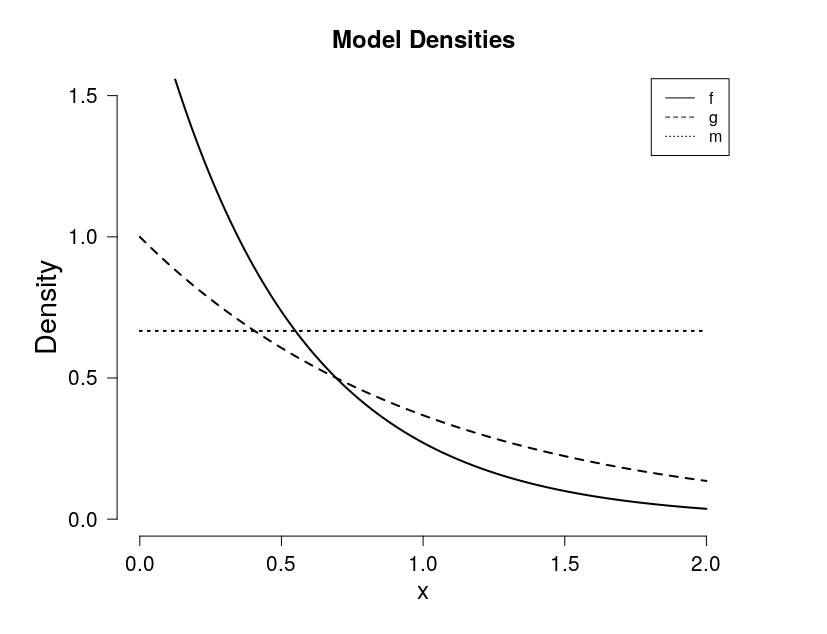
\includegraphics[width=0.65\textwidth]{./figures/exp_exp_dens}
	\end{center}
	\caption{Probability density functions $f$, $g$ and censoring model $m$ for Simulation 1.}
	\label{fig:dens_expexp}
\end{figure}
 Under this setup we have $m(\cdot, \theta) = 2/3$. Since the censoring model is constant, we can expect that censoring will be occurring at the same rate over the whole domain.
\begin{table}[h!]
	\begin{center}
		%run(n = c(500,1000,5000), theta1 = c(2,1), theta2 = c(1,1))
		\begin{tabular}{| l || c | c | c |}
			\hline
			&       $n=100$   &    $n=500$    &    $n=1000$\\
			\hline
			\hline
			%			$\sigma_n^{se}$ & 0.191866 & 0.218288 & 0.229699\\
			%			$\sigma_n^{km}$ & 0.180889 & 0.213888 & 0.223222\\
			%			$\sigma_n^{cl}$ & 0.219298 & 0.232127 & 0.241302\\
			%			\hline
			$Bias(\sigma_n^{se})$ & -0.058134 & -0.031712 & -0.020301\\
			$Bias(\sigma_n^{km})$ & -0.069111 & -0.036112 & -0.026778\\
			$Bias(\sigma_n^{cl})$ & -0.030702 & -0.017873 & -0.008698\\
			\hline
			$Var(\sigma_n^{se})$ & 0.005358 & 0.002032 & 0.001306\\
			$Var(\sigma_n^{km})$ & 0.009067 & 0.002828 & 0.001783\\
			$Var(\sigma_n^{cl})$ & 0.007999 & 0.002731 & 0.001645\\
			\hline
			$MSE(\sigma_n^{se})$ & 0.008737 & 0.003038 & 0.001719\\
			$MSE(\sigma_n^{km})$  & 0.013843 & 0.004132 & 0.0025\\
			$MSE(\sigma_n^{cl})$ & 0.008942 & 0.003051 & 0.001721\\
			\hline
			\hline
			$\bar c$  &0.6646 & 0.66456 & 0.66831\\
			\hline
		\end{tabular}
	\end{center}
	\caption{Results for Simulation 1.}
	\label{tab:res_expexp1}
\end{table}\\
%
Table \ref{tab:res_expexp1} shows, that bias, variance and MSE are decreasing to zero for all three estimators. $\sigma_n^{se}$ and $\sigma_n^{cl}$ are performing clearly better than $\sigma_n^{km}$ under this setup, while $\sigma_n^{se}$ and $\sigma_n^{cl}$ show roughly the same behavior, as we expected in the beginning of this section. 
\begin{figure}[h!]
	\begin{center}
		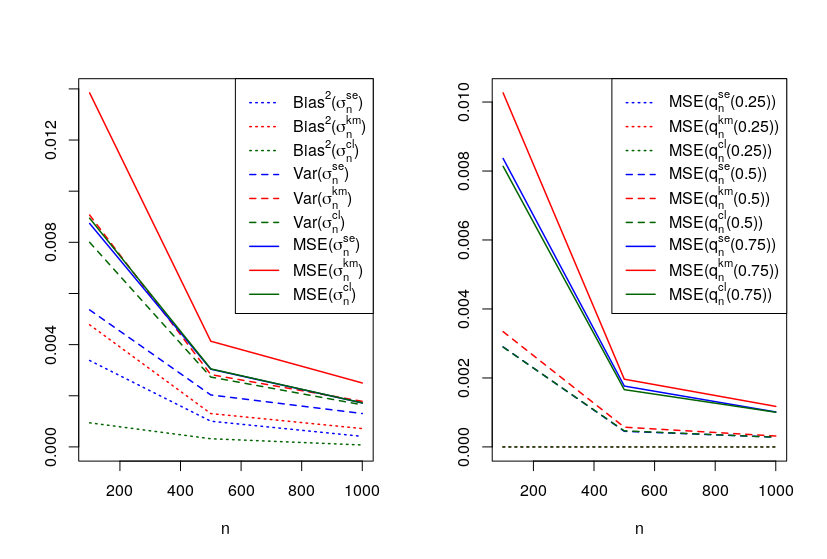
\includegraphics[width=0.85\textwidth]{./figures/expexp_mse2}
	\end{center}
	\caption{Results for Simulation 1. left: bias, variance and MSE for $\sigma_n^{se}$ and $\sigma_n^{km}$. right: MSE for $q_n^{se}$ and $q_n^{km}$.}
	\label{fig:mse_expexp}
\end{figure}
%
\clearpage
%
Figure \ref{fig:mse_expexp} indicates that the gain in efficiency of $\sigma_n^{se}$ and $\sigma_n^{cl}$ versus $\sigma_n^{km}$ is greater for smaller sample sizes. Moreover we can see that the gain in efficiency for $\sigma_{n}^{se}$ and $\sigma_n^{cl}$ is more related to the variance, than to the bias.\\
\\
The Quantiles are estimated quite well under this setup, though they are mainly underestimated by a small amount. 
%
\begin{table}[h!]
	\begin{center}
		%run(n = c(500,1000,5000), theta1 = c(2,1), theta2 = c(1,1))
		\begin{tabular}{| l || c | c | c || c | c | c |}
			\hline
			&       $n=100$   &    $n=500$    &    $n=1000$ &       $n=100$   &    $n=500$    &    $n=1000$\\
			\cline{2-7}
			& \multicolumn{3}{c||}{$Bias$} &\multicolumn{3}{c|}{$MSE$}\\
			\hline
			\hline
			$q^{se}_n(0.25) $  & -0.010451 & -0.00343 & -0.003073  & 0.000733 & 0.000149 & 0.000079\\
			$q^{km}_n(0.25) $  & -0.003812 & -0.001652 & -0.002311  & 0.000981 & 0.00018 & 0.000088\\
			$q^{cl}_n(0.25) $  & -0.006674 & -0.00119 & -0.001907  & 0.000736 & 0.000137 & 0.000076\\
			\hline
			$q^{se}_n(0.5) $  & -0.010855 & -0.001042 & -0.003221  & 0.002899 & 0.000453 & 0.000283\\
			$q^{km}_n(0.5)$  & -0.004584 & -0.000072 & -0.001659  & 0.003342 & 0.000572 & 0.000316\\
			$q^{cl}_n(0.5)$  & -0.008816 & 0.000637 & -0.002438  & 0.002894 & 0.000465 & 0.000281\\
			\hline
			$q^{se}_n(0.75)$  & -0.012331 & 0.00739 & -0.003152  & 0.008363 & 0.001764 & 0.001012\\
			$q^{km}_n(0.75)$  & -0.014291 & 0.007734 & -0.003026  & 0.010265 & 0.001963 & 0.001175\\
			$q^{cl}_n(0.75)$  & -0.019053 & 0.003871 & -0.004781  & 0.008135 & 0.00166 & 0.001006\\
			\hline
		\end{tabular}
	\end{center}
	\caption{Results for estimated quantiles of Simulation 1.}
	\label{tab:res_expexp2}
\end{table}
%
%\clearpage
%
%
%
\section{Simulation 2} \label{sec:sim_weiwei}

Let $X \sim Weibull(\alpha_1, \beta_1)$ and  $X \sim Weibull(\alpha_2, \beta_2)$.
%$$f(z) = \alpha_1\beta_1 (\alpha_1 z)^{\beta_1-1}\exp\left(-(\alpha_1 z)^{\beta_1}\right)$$
%$$g(z) = \alpha_2\beta_2 (\alpha_2 z)^{\beta_2-1}\exp\left(-(\alpha_2 z)^{\beta_2}\right)$$
Then we obtain for the censoring model 
$$m(z,\theta) = \frac{1}{1+\theta_1 z^{\theta_2}} \textrm{ with } \theta = \left(\frac{\alpha_2^{\beta_2}\beta_2}{\alpha_1^{\beta_1}\beta_1}, \beta_2 - \beta_1\right)$$
%
For the simulation below we chose $\alpha_1 = 2$, $\alpha_2 = 1$, $\beta_1 = 1.2$ and $\beta_2 = 1$. The target value was here
$$Var(X) = 0.192843\mdot$$
Figure \ref{fig:dens_wei_wei} indicates that smaller values are censored rather than larger ones under this setup.  This is due to the increasing nature of the censoring model $m$.
%
\clearpage
%
\begin{figure}[h!]
	\begin{center}
		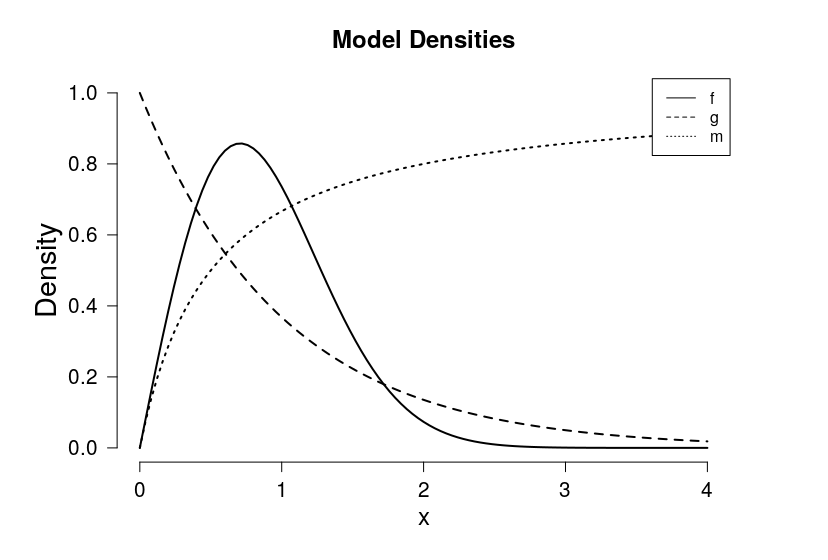
\includegraphics[width=0.65\textwidth]{./figures/wei_wei_dens}
	\end{center}
	\caption{Probability density functions $f$, $g$ and censoring model $m$ for Simulation 1.}
	\label{fig:dens_wei_wei}
\end{figure}
\noindent Table \ref{tab:res_weiwei1} shows that bias, variance and MSE are converging to zero for both estimators, as well under this setup. The semiparametric estimator is clearly more efficient than the Kaplan-Meier estimate \wrt\ the MSE. Here again, difference in variance is much larger than the difference in squared bias. 
%
\begin{table}[h!]
	\begin{center}
		%run(n = c(500,1000,5000), theta1 = c(2,1.2), theta2 = c(1,1))
		\begin{tabular}{| l || c | c | c |}
			\hline
			&       $n=100$   &    $n=500$    &    $n=1000$\\
			\hline
			\hline
%			$Var$ & 0.154936 & 0.154936 & 0.154936\\
%			$U_n^{se}$ & 0.13533 & 0.154696 & 0.158717\\
%			$U_n^km$ & 0.134849 & 0.143497 & 0.143514\\
			$Bias(\sigma_n^{se})$ & -0.019606 & -0.000239 & 0.003782\\
			$Bias(\sigma_n^{km})$ & -0.020086 & -0.011439 & -0.011422\\
			\hline
			$Var(\sigma_n^{se})$ & 0.001659 & 0.000669 & 0.000298\\
			$Var(\sigma_n^{km})$ & 0.002861 & 0.000794 & 0.000257\\
			\hline
			$MSE(\sigma_n^{se})$ & 0.002044 & 0.000669 & 0.000312\\
			$MSE(\sigma_n^{km})$ & 0.003265 & 0.000925 & 0.000388\\
			\hline
			\hline
			$\bar c$ & 0.6705 & 0.6678 & 0.66538\\
			\hline
		\end{tabular}
	\end{center}
	\caption{Results for Simulation 2.}
	\label{tab:res_weiwei1}
\end{table}\\
%
Figure \ref{fig:mse_weiwei} shows, as before, that the gain in efficiency is greater for smaller sample sizes $n$. Again, the gain in efficiency is more severe for smaller $n$ in this simulation. We can also see that the variance is contributing more to the gain in efficiency.
%
\clearpage
%
\begin{figure}[h]
	\begin{center}
		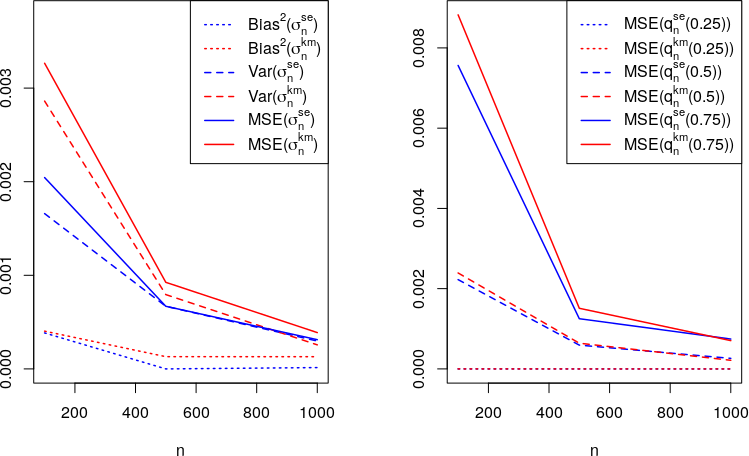
\includegraphics[width=0.85\textwidth]{./figures/weiwei_mse2}
	\end{center}
	\caption{Results for Simulation 2. left: bias, variance and MSE for $\sigma_n^{se}$ and $\sigma_n^{km}$. right: MSE for $q_n^{se}$ and $q_n^{km}$.}
	\label{fig:mse_weiwei}
\end{figure}
%
\noindent The Quantiles are estimated quite well under this setup, as we can see from Table \ref{tab:res_weiwei2}. As before, the quantiles are, for the most part, slightly underestimated by both estimators. Figure \ref{fig:mse_weiwei} shows that $q_n^{se}$ is performing slightly better $q_n^{km}$ here.
\begin{table}[h!]
	\begin{center}
		%run(n = c(500,1000,5000), theta1 = c(2,1.2), theta2 = c(1,1))
		\begin{tabular}{| l || c | c | c || c | c | c |}
			\hline
			&       $n=100$   &    $n=500$    &    $n=1000$ &       $n=100$   &    $n=500$    &    $n=1000$\\
			\cline{2-7}
			& \multicolumn{3}{c||}{$Bias$} &\multicolumn{3}{c|}{$MSE$}\\
			\hline
			\hline
			$q^{se}_n(0.25)$ & -0.018255 & -0.011443 & -0.011854& 0.000873 & 0.000228 & 0.000206\\
			$q^{km}_n(0.25)$ & -0.007356 & -0.000332 & -0.000922& 0.000666 & 0.000165 & 0.000079\\
			\hline
			$q^{se}_n(0.5)$ & -0.012298 & -0.011298 & -0.00798& 0.002225 & 0.000593 & 0.000263\\
			$q^{km}_n(0.5)$ & -0.006786 & -0.00582 & -0.002101 & 0.002391 & 0.000641 & 0.000215\\
			\hline
			$q^{se}_n(0.75)$ & -0.009176 & 0.000363 & 0.007358& 0.007562 & 0.001251 & 0.000744\\
			$q^{km}_n(0.75)$ & -0.015825 & -0.010461 & -0.002481 & 0.008823 & 0.001511 & 0.000705\\
			\hline
		\end{tabular}
	\end{center}
	\caption{Results for estimated quantiles of Simulation 2.}
	\label{tab:res_weiwei2}
\end{table}
%
%
%
\section{Simulation 3} \label{sec:sim_exppar}
Let $X \sim Exp(\alpha)$ and $Y \sim Par(\beta)$. For our model $m$ we obtain in this case
$$m(z,\theta) = \frac{\alpha}{\alpha + \frac{\beta}{z}\I{z \geq \beta}}\mdot$$
Note that $m$ is \textbf{not} non-decreasing over the whole domain in this case (\cf\ Example \ref{ex:exppar}). For the following simulation we chose $\alpha = 0.5$ and $\beta = 1.2$. The target value was here
$$Var(X) = 4\mdot$$
%
%\clearpage
%
\begin{figure}[h!]
	\begin{center}
		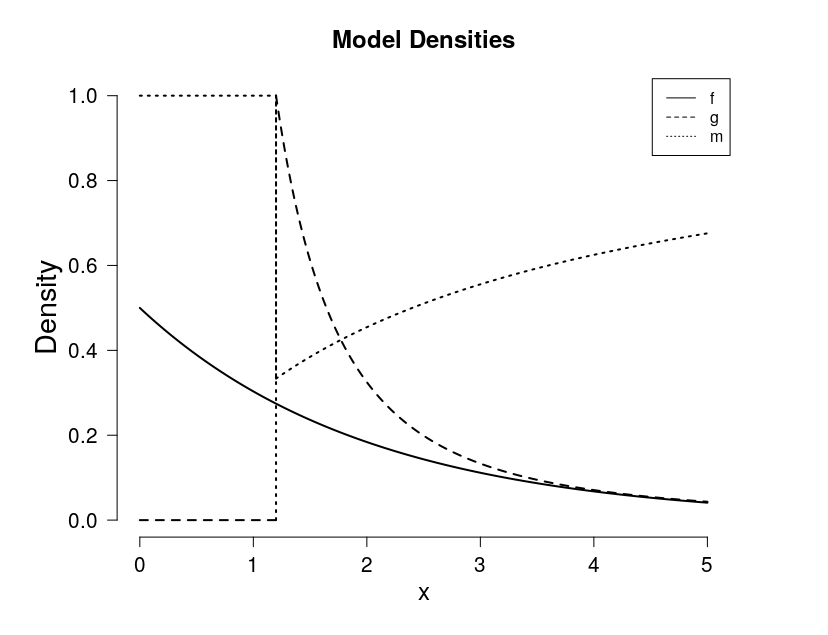
\includegraphics[width=0.65\textwidth]{./figures/exppar_dens}
	\end{center}
	\caption{Probability density functions $f$, $g$ and censoring model $m$ for Simulation 3.}
	\label{fig:dens_exppar}
\end{figure}
%
Considering Figure \ref{fig:dens_exppar}, we can not expect any censored observations on $[0,\beta]$. Moreover the plot indicates that values in $[\beta,3]$ are more likely to be censored. On $[\beta,\infty)$, the censoring model is monotone increasing. This implies that smaller values are more likely to be censored than larger values.
\clearpage
\begin{table}[h!]
	\begin{center}

%run(n = c(100,500,1000), m = 100, theta = c(0.5, 1.2))
	\begin{tabular}{| l || c | c | c |}	
		\hline
		& $ n = 100 $ & $ n = 500 $ & $ n = 1000 $\\
		\hline
		\hline
%		$Var$ & 4 & 4 & 4\\
%		$U_n^{se}$ & 2.938322 & 3.574439 & 3.726535\\
%		$U_n^km$ & 2.902828 & 3.48581 & 3.681142\\
		$Bias(\sigma_n^{se})$ & -1.061678 & -0.425561 & -0.273465\\
		$Bias(\sigma_n^{km})$ & -1.097172 & -0.51419 & -0.318858\\
		\hline
		$Var(\sigma_n^{se})$ & 2.828115 & 0.852244 & 0.362266\\
		$Var(\sigma_n^{km})$ & 2.991916 & 1.289473 & 0.5611\\
		\hline
		$MSE(\sigma_n^{se})$ & 3.955275 & 1.033346 & 0.437049\\
		$MSE(\sigma_n^{km})$ & 4.195703 & 1.553865 & 0.66277\\
		\hline
		\hline
		$\bar c$ & 0.6971 & 0.69704 & 0.69616\\
		\hline
	\end{tabular}
	\end{center}
	\caption{Results for simulation 3.}
	\label{tab:res_exppar1}
\end{table}
%
\noindent From Table \ref{tab:res_exppar1}, we see that the MSE values of both estimators,  $\sigma_n^{se}$ and $\sigma_n^{km}$, are substantially larger than in the previous examples, especially for $n=100$. However, the MSE values decrease considerably as $n$ increases. Figure \ref{fig:mse_exppar}, shows that the semiparametric estimator is performing better than the Kaplan-Meier estimate again, with a larger gain in efficiency for small $n$ .
\begin{figure}[h!]
	\begin{center}
		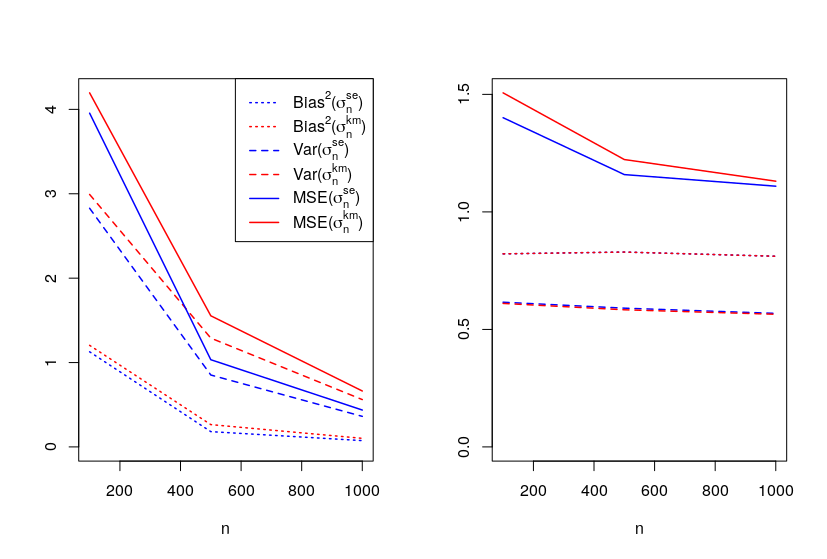
\includegraphics[width=0.8\textwidth]{./figures/exppar_mse2}
	\end{center}
	\caption{Results for Simulation 3. left: bias, variance and MSE for $\sigma_n^{se}$ and $\sigma_n^{km}$. right: MSE for $q_n^{se}$ and $q_n^{km}$.}
	\label{fig:mse_exppar}
\end{figure}
%
\clearpage
Table \ref{tab:res_exppar2} shows, that the quantiles are considerably substantially by both estimators in this case. This might be a consequence of the fact, that $m$ violates condition (A\ref{ass:m_increas}) under this setup. The large MSE values for the quantile estimates are likely to cause the much larger MSE scores of $\sigma_n^{se}$ and $\sigma_n^{km}$ for this simulation.
\begin{table}[h!]
	\begin{center}
		
		%run(n = c(100,500,1000), m = 100, theta = c(0.5, 1.2))
		\begin{tabular}{| l || c | c | c || c | c | c |}
			\hline
			&       $n=100$   &    $n=500$    &    $n=1000$ &       $n=100$   &    $n=500$    &    $n=1000$\\
			\cline{2-7}
			& \multicolumn{3}{c||}{$Bias$} &\multicolumn{3}{c|}{$MSE$}\\
			\hline
			\hline
			$q^{se}_n(0.25)$ & -0.946058 & -0.953076 & -0.948244& 0.906359 & 0.910549 & 0.900719\\
			$q^{km}_n(0.25)$ & -0.946058 & -0.953076 & -0.948244& 0.906359 & 0.910549 & 0.900719\\
			\hline
			$q^{se}_n(0.5)$ & -0.761661 & -0.763693 & -0.751274& 0.615678 & 0.590391 & 0.568224\\
			$q^{km}_n(0.5)$ & -0.756513 & -0.758938 & -0.748412 & 0.610569 & 0.583492 & 0.564373\\
			\hline
			$q^{se}_n(0.75)$ & -1.144379 & -1.062969 & -1.04613 & 1.400626 & 1.158716 & 1.109287\\
			$q^{km}_n(0.75)$ & -1.164122 & -1.088963 & -1.0535 & 1.506353 & 1.222739 & 1.130558\\
			\hline
		\end{tabular}
	\end{center}
	\caption{Results for estimated quantiles of Simulation 3.}
	\label{tab:res_exppar2}
\end{table}

	\cleardoublepage
	
	\chapter{Conclusion}
\todo{Conclusion goes here...}
\begin{itemize}
	\item Summarize the SLLN for semiparametric U-Statistics
	\item Discussion of main assumptions and examples of kernels $\phi$ and censoring models $m$
	\item Future (or perhaps in this thesis): Transfer that property to Prof. Dikta's new estimator using stochastic equivalence
	\item Future: CLT based on \cite{bose2002asymptotic}
\end{itemize}

	\cleardoublepage
	
	%-----------------------
	
	%%%%%%%%%%%%%%%%%%%%%%%%%%%%%%
	%%%%%%%% Bibliography %%%%%%%%
	%%%%%%%%%%%%%%%%%%%%%%%%%%%%%%
		
	% Formatting the bibliography pages
	\backmatter 
	
	%-----------------------
	
	% Adding Bibliography entry to table of contents
	\addcontentsline{toc}{chapter}{\ \quad \textbf{Bibliography}}
	
	%-----------------------
	
	% The "\bibliographystyle" argument refers to the file (in .bst format) containing a specific citation style file.  Templates can typically be obtained from publication websites, such as the American Geophysical Union (www.agu.org), the American Meteorological Society (www.ametsoc.org), or other publishers.
	
	% Please make sure that your citation style is appropriate for your field, and that it follows standard style guidelines.
	
	% The "\bibliography" argument refers to the file (in .bib format) where your BiBTeX citations are located.  Be sure to include the entire path to the file, to avoid errors.
	
	% UNCOMMENT THIS SECTION IF YOU WISH TO USE BiBTeX
	% Change this argument to match your bibliography style file
	\bibliographystyle{./ametsoc}
	%\bibliographystyle{alphanum}
	
	% Generate the bibliography using entries from the following .BIB file
	\bibliography{./thesis}
	%-----------------------
	
	% BEGINNING OF APPENDIX SECTION.
	% IF YOU DO NOT WISH TO HAVE AN APPENDIX, COMMENT THIS ENTIRE SECTION OUT!
	\ThesisAppendix
	
	% Resetting the equation and table counters to zero.  DO NOT DELETE!
	%\setcounter{equation}{0}
	%\setcounter{table}{0}
	
	% Adding an A in front of any equation numbers or table numbers in the appendix.  DO NOT DELETE!
	\renewcommand{\theequation}{A\arabic{equation}}
	\renewcommand{\thetable}{A\arabic{table}}
	\renewcommand{\thethm}{A.\arabic{thm}}
	
	% Creating a new chapter (the asterisk tells LaTeX not to number the chapter)
\chapter{Appendix: Supplementary Results}
	\begin{lemma} \label{lem:bounds}
		For $n\geq 2$ the following statements hold true
		\begin{enumerate}[(i)]
			\item \begin{equation}
			\sum_{k=1}^{n-1} \frac{1}{k} \leq \ln(n-1) + 1
			\label{eq:sum_ln}
			\end{equation}
			%
			\item \begin{equation}
			\frac{\ln(n-1)+1}{(n+1)^{\frac{1}{3}}} \leq 3
			\label{eq:ln_over_n_upperb}
			\end{equation}
		\end{enumerate}
		%	
		\begin{proof}
			We will start with the proof of part (i). Consider 
			\begin{align*}
			& \quad\sum_{k=1}^{n-1} \frac{1}{k} \quad \leq \quad  \ln(n-1) + 1 \\
			\Leftrightarrow & \quad \sum_{k=1}^{n-1} \frac{1}{k} - 1 \quad \leq \quad  \ln(n-1)\\
			\Leftrightarrow & \quad \sum_{k=2}^{n-1} \frac{1}{k} \quad \leq \quad  \ln(n-1)
			\numberthis\label{eq:prodexp}
			\end{align*}
			%
			Moreover we have
			\begin{align*}
			\sum_{k=2}^{n-1} \frac{1}{k} &= \sum_{k=2}^{n-1} \int_{k-1}^{k}\frac{1}{k} dx\\
			&\leq \sum_{k=2}^{n-1} \int_{k-1}^{k}\frac{1}{x} dx\\
			&\leq \sum_{k=2}^{n-1} \ln(k) - \ln(k-1)\\
			&\leq \ln(n-1) - \ln(1)\\
			&= \ln(n-1)
			\end{align*}
			Thus proving part (i). 
			%
			We will continue with the proof of part (ii). Note that \eqref{eq:ln_over_n_upperb} is equivalent to showing 
			\begin{equation*}
			\ln(n-1)+1 \leq 3(n+1)^{\frac{1}{3}}
			\end{equation*}
			%
			Since $\ln(n-1)\leq \ln(n+1)$, this will be implied by the following
			\begin{equation}
			\ln(n+1)+1 \leq 3(n+1)^{\frac{1}{3}}
			\label{eq:ln_root}
			\end{equation}
			It is easy to check that inequality \eqref{eq:ln_root} holds for $n=2$. Now consider that 
			$$\frac{d}{dn}(\ln(n+1)+1) = \frac{1}{n+1}$$
			and
			$$\frac{d}{dn} 3(n+1)^\frac{1}{3} = \frac{1}{(n+1)^\frac{2}{3}}$$
			to get
			\begin{equation}
			\frac{d}{dn}(\ln(n+1)+1) \leq \frac{d}{dn} 3(n+1)^\frac{1}{3}
			\label{eq:derivs}
			\end{equation}	
			for all $n\geq 2$. Now the result in (ii) follows directly from \eqref{eq:ln_root} and \eqref{eq:derivs} .
		\end{proof}
	\end{lemma}
%
\chapter{Appendix: Thoughts on finding weaker assumptions}

In Section \ref{sec:not_supermart}, we were only able to show that $S_n(q)$ is a reverse supermartingale under the assumption that $q$ is monotone increasing. To establish the almost sure existence of limits of supermartingale processes, one considers the number of upcrossings of an interval $[a,b]$ by the process. This was done in the famous Upcrossing Theorem by Doob \todo{cite}. During this section we will generalize Doob's Upcrossing Theorem to our framework in order to explore ways to establish weaker assumptions. To get closer to the situation of Doob's Upcrossing Theorem, we define the following quantities. Let $N<\infty$ and define for $1\leq n\leq N$ 
\begin{equation*}
\StN{n} := \sn{N-n+1} \textrm{, } \FtN{n} := \F_{N-n+1} \textrm{ \ and \ } \xitN{n} := \xi_{N-n+1}\mdot
\end{equation*}
Note that $\{\FtN{n}\}_{1\leq n\leq N}$ is now an increasing $\sigma$-field in $n$.
%
Below we will define everything needed, in order to generalize Doob's Upcrossing Theorem.
\begin{defn}
	Let $N\geq 2$. For $1\leq n\leq N$ and $a, b \in \mathbb{R}$ with $a < b$, let 
	\begin{align*}
	T_0 &:= 0\\
	T_1 &:= \begin{cases} 
	\min\{1\leq n\leq N | \StN{n}\leq a\} & \textrm{ if } \{1\leq n\leq N | \StN{n}\leq a\}\neq \emptyset\\
	N & \textrm{ if } \{1\leq n\leq N | \StN{n}\leq a\}= \emptyset
	\end{cases}\\	
	T_2 &:= \begin{cases} 
	\min\{T_1\leq n\leq N | \StN{n}\geq b\} & \textrm{ if } \{T_1\leq n\leq N | \StN{n}\leq a\}\neq \emptyset\\
	N & \textrm{ if } \{T_1\leq n\leq N | \StN{n}\geq b\} = \emptyset
	\end{cases}\\	
	\vdots &\quad \vdots \quad \vdots	\\
	T_{2m-1} &:= \begin{cases} 
	\min\{T_{2m-2}\leq n\leq N | \StN{n}\leq a\} & \textrm{ if } \{T_{2m-2}\leq n\leq N | \StN{n}\leq a\}\neq \emptyset\\
	N & \textrm{ if } \{T_{2m-2}\leq n\leq N | \StN{n}\leq a\}= \emptyset
	\end{cases}\\	
	T_{2m} &:= \begin{cases} 
	\min\{T_{2m-1}\leq n\leq N | \StN{n}\geq b\} & \textrm{ if } \{T_{2m-1}\leq n\leq N | \StN{n}\leq a\}\neq \emptyset\\
	N & \textrm{ if } \{T_{2m-1}\leq n\leq N | \StN{n}\geq b\} = \emptyset
	\end{cases}\mdot
	\end{align*}
	%
	Now we can define the number of upcrossings of $[a, b]$ by $\StN{1}, ..., \StN{n}$ as follows:
	\[
	\UNab{n} :=\begin{cases}  
	\max\{1\leq m \leq N | T_{2m} < N\} & \textrm{ if } \{1\leq m \leq N | T_{2m} < N\}\neq \emptyset\\
	0 &  \textrm{ if } \{1\leq m \leq N | T_{2m} < N\} = \emptyset
	\end{cases}
	\]
	%
	Furthermore let for $1\leq k\leq n-1$
	\[ \epsilon_k := \begin{cases} 
	0 & \textrm{ if } k < T_1 \\
	1 & \textrm{ if } T_1 \leq k < T_2\\
	0 & \textrm{ if } T_2 \leq k < T_3\\
	1 & \textrm{ if } T_3 \leq k < T_4\\
	\dots & \textrm{ if } \dots
	\end{cases}
	\]
	and define
	$$\YN{n} := \StN{1} + \sum\limits_{k=1}^{n-1} \epsilon_k (\StN{k+1}-\StN{k})$$
	for $1\leq n\leq N$. 	
\end{defn}
%
Let's now explore how $\lim_{N\to\infty}\UNab{N}<\infty$ implies that $S$ must exist amost surely. Suppose for now, that $\lim_{N\to\infty}\UNab{N}<\infty$ and define the set of all $\omega$ for which $S_n$ does not converge as
$$\Lambda := \{\omega | S_n(\omega) \textrm{ does not converge}\}\mdot$$
%
Consider that can write
\begin{align*}
\Lambda &= \{\omega | \liminf_{n}S_n(\omega) < \limsup_{n} S_n(\omega)\}\\
&= \bigcup_{a,b\in\mathbb{Q}}\{\omega | \liminf_{n}S_n(\omega) < a < b < \limsup_{n} S_n(\omega)\}\mdot
\end{align*}
%  
Recall that we have $\UNab{N}$, the number of upcrossings of $[a,b]$ by $\StN{1}, \dots, \StN{N}$. But this is equal to the number of upcrossings of $[a,b]$ by $S_N, \dots, S_1$. Furthermore recall that 
$$U_\infty[a,b] = \lim\limits_{N\to\infty} \UNab{N}\mdot$$
%
Consider that for each $\omega \in \{\omega | \liminf_{n}S_n(\omega) < a < b < \limsup_{n} S_n(\omega)\}$ we must have $U_{\infty}[a,b](\omega) = \infty$. This follows directly from the definitions of $\liminf$ and $\limsup$. Thus we can write
\begin{equation*}
\Lambda = \bigcup_{a,b\in\mathbb{Q}}\{ \omega | U_\infty[a,b](\omega) = \infty\} = \bigcup_{a,b\in\mathbb{Q}} \Lambda_{a,b}
\end{equation*}
where $\Lambda_{a,b} := \{ \omega | U_\infty[a,b](\omega) = \infty\}$.
%
Consequently we get that
\begin{equation}
\E[\I{\Lambda_{a,b}} U_\infty[a,b]] = \begin{cases}
\infty &\textrm{ if } \P(\Lambda_{a,b})>0\\
0 &\textrm{ if } \P(\Lambda_{a,b})=0\\
\end{cases}\mdot
\label{eq:lambda_u}
\end{equation}
%
Note that $\UNab{N}$ is clearly non-decreasing in $N$. Now if $\lim_{N\to\infty}\E[\UNab{N}]<\infty$, we can apply the Monotone Convergence Theorem  to obtain
$$\lim\limits_{N\to\infty}\E[\UNab{N}] = \E[U_\infty[a,b]] <\infty$$	
%	
and hence that
$$\E[\I{\Lambda_{a,b}} U_\infty[a,b]] \leq \E[U_\infty[a,b]] < \infty\mdot$$
%
Now the latter together with \eqref{eq:lambda_u} implies that $\P(\Lambda_{a,b}) = 0$. Therefore we have
\begin{equation*}
\P(\Lambda) = \P\left(\bigcup_{a,b\in\mathbb{Q}}\Lambda_{a,b}\right) = \sum_{a,b \in \mathbb{Q}} \P(\Lambda_{a,b}) = 0 \mdot
\end{equation*}
%
%
%
The following Lemmas show how Doob's Upcrossing Theorem can be adapted to our framework. We will show that $\E[\UNab{n}]$ is bounded above by $\E[Y_n^N]/(b-a)$.
\begin{lemma}
	For $1\leq n\leq N$ we have
	$$\E[\UNab{n}]\leq \frac{\E[\YN{n}]}{b-a}\mdot$$
	\label{lem:upcrossings_yn}
\end{lemma}
%
\begin{proof}
	Consider for $1\leq n\leq N$ and $N\geq 2$
	\begin{align*}
	Y_n^N &= \StN{1} + \sum_{k=1}^{n-1}\epsilon_k(\StN{k+1}-\StN{k})\\
	&= \StN{1} + \sum_{k=1}^{n}(\StN{T_{2k}}-\StN{T_{2k-1}})\\
	&\geq \sum_{k=1}^{n}(\StN{T_{2k}}-\StN{T_{2k-1}})
	\end{align*}
	by definition of $\epsilon_k$. The latter inequality above holds, since $\StN{1}\geq 0$. Note that by definition of $T_1, T_2, \dots$ we have
	$$\sum_{k=1}^{n}(\StN{T_{2k}}-\StN{T_{2k-1}}) \geq (b-a)\UNab{n}\mdot$$
	From here the assertion follows directly.
\end{proof}
%
The following lemma provides a representation for the expectation of the process $Y_N^n$.
\begin{lemma}
	\label{lem:optional_skipping}
	For $1\leq n\leq N$ let
	$$\YN{n} := \StN{1} + \sum_{k=1}^{n-1} \epsilon_k (\StN{k+1} - \StN{k}) $$
	with
	\[ \epsilon_k := \begin{cases} 
	1 & (\StN{1},\dots,\StN{k})\in B_k \\
	0 & otherwise 
	\end{cases}
	\]
	for $k=1,\dots, n-1$. Here $B_k$ is an arbitrary set in $\mathfrak{B}(\mathbb{R}^k)$. Then we have
	\begin{equation}
	\E[\YN{n}] = \E[\StN{n}] - \sum_{k=1}^{n-1}\E\left[(1-\epsilon_k)\left(\E[\StN{k+1}|\FtN{k}]  - \StN{k} \right)\right]\mdot
	\label{eq:ineq_yk}
	\end{equation}
\end{lemma}
%
\begin{proof}
	Consider for $1\leq n\leq N$ and $N\geq 2$
	\begin{align*}
	&  \StN{n+1} - \YN{n+1} \\ 
	&= (1-\epsilon_1)(\StN{2} - \StN{1}) + (1-\epsilon_2)(\StN{3} - \StN{2}) + ... + (1-\epsilon_k)(\StN{n+1} - \StN{n})\\ 
	&= (\StN{n} - \YN{n}) + (1-\epsilon_n)(\StN{n+1} - \StN{n}) \mdot
	\end{align*}
	%
	Conditioning on $\FtN{n}$ on both sides yields
	\begin{align*}
	\E[\StN{n+1} - \YN{n+1}|\FtN{n}] &= \StN{n} - \YN{n} + (1-\epsilon_n)\left(\E[(\StN{n+1})|\FtN{n}]  - \StN{n} \right)\mdot
	\end{align*}
	\\
	Now taking expectations on both sides yields
	$$\E[\StN{n+1} - \YN{n+1}] \geq \E[\StN{n} - \YN{n}] + \E\left[(1-\epsilon_n)\left(\E[\StN{n+1}|\FtN{n}]  - \StN{n} \right)\right]\mdot$$
	Note that 
	\begin{align*}
	\E[\StN{2} - \YN{2}] &= \E[\StN{1} - \YN{1}] + \E\left[(1-\epsilon_1)\left(\E[\StN{2}|\FtN{1}]  - \StN{1} \right)\right]\\ 
	&= \E\left[(1-\epsilon_1)\left(\E[\StN{2}|\FtN{1}]  - \StN{1} \right)\right]\\ 
	\end{align*}
	since $\YN{1} = \StN{1}$. Moreover we have
	\begin{align*}
	\E[\StN{3} - \YN{3}] &= \E[\StN{2} - \YN{2}] + \E\left[(1-\epsilon_2)\left(\E[\StN{3}|\FtN{2}]  - \StN{2} \right)\right]\\  
	&= \E\left[(1-\epsilon_1)\left(\E[\StN{2}|\FtN{1}]  - \StN{1} \right)\right]\\
	&\qquad + \E\left[(1-\epsilon_2)\left(\E[\StN{3}|\FtN{2}]  - \StN{2} \right)\right]\\  
	&\cdots& \\ 
	\E[\StN{n} - \YN{n}] &= \sum_{k=1}^{n-1}\E\left[(1-\epsilon_k)\left(\E[\StN{k+1}|\FtN{k}]  - \StN{k} \right)\right]\mdot
	\end{align*}
	%
	Hence we get
	\begin{equation*}
	\E[\YN{n}] = \E[\StN{n}] - \sum_{k=1}^{n-1}\E\left[(1-\epsilon_k)\left(\E[\StN{k+1}|\FtN{k}]  - \StN{k} \right)\right]\mdot
	\end{equation*}	
\end{proof}
%
\begin{remark}
	Note that we have $\YN{1}=\StN{1}$, as the sum in the definition above is in this case empty and hence treated as zero. Moreover note that we have $\YN{n+1} = \StN{n+1}$ if $\epsilon_k=1$ for all $1\leq k \leq n$. 
\end{remark}
%
The Lemma below establishes an upper bound for $\E[Y_N^N]$ in terms of $Q_{ij}^{N-k+1}$, as defined in Lemma \ref{lem:qi}. 
\begin{lemma} \label{lem:cs}
	We have for $N\geq 2$
	\begin{align*}
	\E[Y_N^N] &\leq \E[\StN{N}] + \sum_{k=1}^{N-1} \alpha_{N-k+1} \numberthis\label{eq:yn}
	\end{align*}
	where
	\begin{align*}
	\alpha_{N-k+1} &:= \doublesum\limits_{1\leq i<j\leq N-k+1}\E\left[\phi(Z_{i:N-k+1}, Z_{j:N-k+1}) W_{i:N-k+1} W_{j:N-k+1}(Q_{i,j}^{N-k+1} - 1)\right]\mdot
	\end{align*}
	%
	\begin{proof}
		Combining Lemmas \ref{lem:optional_skipping} and \ref{lem:upcrossings_yn} yields the following for $n\leq N$
		$$(b-a) \E[U_n[a,b]] \leq \E[Y_n^N] = \E[\StN{n}] - \sum_{k=1}^{n-1} \E[(1-\epsilon_k) \left(\E[\StN{k+1} | \F_k^N] - \StN{k}\right)]\mdot$$
		%
		Moreover we get from Lemma \ref{lem:qi}
		\begin{align*}
		\E[\StN{k+1}|\FtN{k}] &= \E[\sn{N-k} | \F_{N-k+1}]\\
		&= \doublesum\limits_{1\leq i<j\leq N-k+1} \phi(Z_{i:N-k+1}, Z_{j:N-k+1}) W_{i:N-k+1} W_{j:N-k+1} Q_{i,j}^{N-k+1}\mdot
		\end{align*}
		%
		Therefore we obtain
		\begin{align*}
		\E[Y_N^N] &= \E[\StN{N}] - \sum_{k=1}^{N-1} \E[(1-\epsilon_k) \E[\StN{k+1} | \F_k^N] - \StN{k} ]\\
		&=  \E[\StN{N}] - \sum_{k=1}^{N-1} \doublesum\limits_{1\leq i<j\leq N-k+1} \E\left[(1-\epsilon_k)\phi(Z_{i:N-k+1}, Z_{j:N-k+1}) \right. \\
		&\qquad\qquad\qquad\qquad\qquad\qquad \times \left. W_{i:N-k+1} W_{j:N-k+1}(Q_{i,j}^{N-k+1} - 1) \right]\\
		&\leq  \E[\StN{N}] + \left|\sum_{k=1}^{N-1} \doublesum\limits_{1\leq i<j\leq N-k+1} \E\left[(1-\epsilon_k)\phi(Z_{i:N-k+1}, Z_{j:N-k+1}) \right.\right. \\
		&\qquad\qquad\qquad\qquad\qquad\qquad \times \left.\left. W_{i:N-k+1} W_{j:N-k+1}(Q_{i,j}^{N-k+1} - 1) \right]\vphantom{\doublesum\limits_{1\leq i<j\leq N-k+1}}\right|\\
		&\leq  \E[\StN{N}] + \sum_{k=1}^{N-1} \doublesum\limits_{1\leq i<j\leq N-k+1} \left|\E\left[(1-\epsilon_k)\phi(Z_{i:N-k+1}, Z_{j:N-k+1}) \right.\right. \\
		&\qquad\qquad\qquad\qquad\qquad\qquad \times \left.\left. W_{i:N-k+1} W_{j:N-k+1}(Q_{i,j}^{N-k+1} - 1) \right]\right|\mdot
		\end{align*}
		%
		Now using Jensen's inequality yields
		\begin{align*}
		\E[Y_N^N] &\leq \E[\StN{N}] + \sum_{k=1}^{N-1} \doublesum\limits_{1\leq i<j\leq N-k+1}\E\left[(1-\epsilon_k) \phi(Z_{i:N-k+1}, Z_{j:N-k+1}) \right.\\
		&\qquad\qquad\qquad\qquad\qquad\qquad \times \left. W_{i:N-k+1} W_{j:N-k+1} \cdot \abs{(Q_{i,j}^{N-k+1} - 1)}\right]\\
		&\leq \E[\StN{N}] + \sum_{k=1}^{N-1} \doublesum\limits_{1\leq i<j\leq N-k+1}\E\left[\phi(Z_{i:N-k+1}, Z_{j:N-k+1}) \right. \\
		&\qquad\qquad\qquad\qquad\qquad\qquad \times \left. W_{i:N-k+1} W_{j:N-k+1} \cdot \abs{(Q_{i,j}^{N-k+1} - 1)}\right]\mdot
		\end{align*}
		The latter inequality above holds, because $1-\epsilon_k \leq 1$ for all $k\leq N-1$. 
		%
	\end{proof}
\end{lemma}
%
In addition to the almost sure existence of $S(q)$ we need the following statement 
$$S = \lim\limits_{n\to\infty} S_n = \lim\limits_{n\to\infty}\E[S_n]$$
in order to identify $S(q)$ in Lemma \ref{lem:sn_limit}. This could be established by the following Lemma.
\begin{lemma}
	The following statement holds true:
	$$S_\infty = \lim\limits_{n\to\infty} \E[S_n| \F_\infty] = \lim\limits_{n\to\infty}\E[S_n]$$
	almost surely, if the limits above exist.
	\label{lem:connector}
	
	\begin{proof}
		Let $a>0$ and note that, since $S_n\to S$ almost surely as $n\to\infty$, we have
		$$\lim\limits_{n\to\infty}\min(S_n, a) = \min(S,a)$$ 
		almost surely, since $\min(\cdot, a)$ is continuous (see \cite{van2000asymptotic}, Theorem 2.3). Now $\min(S_n,a)$ is bounded by $a$. Hence applying the Dominated Convergence Theorem yields
		\begin{align*}
		\lim\limits_{n\to\infty} \E[\min(S_n,a)|\F_\infty] &= \E[\lim\limits_{n\to\infty} \min(S_n,a)|\F_\infty] \nonumber\\
		&= \E[\min(S_\infty,a)|\F_\infty]\mdot
		%&= \min(S_\infty,a) \numberthis	\label{eq:dom_conv_1}\\
		\end{align*}
		%
		Note that $S_k$ is measurable with respect to $\F_n$  whenever $k\geq n$, therefore $S_\infty$ must be $\F_n$-measurable for all $n\in\mathbb{N}$. Consequently $S_\infty$ must be $F_\infty$-measurable. Moreover, for $a\in\R$, $\min(\cdot,a)$ is a continuous function. Thus $\min(S_\infty,a)$ is $\F_\infty$-measurable as well. Hence
		$$\lim\limits_{n\to\infty}\E[min(S_n,a)|\F_\infty] = \min(S_\infty,a) $$
		almost surely. Thus we have
		\begin{align*}
		\lim\limits_{n\to\infty} \E[S_n|\F_\infty] &=  \lim\limits_{n\to\infty}\lim\limits_{a\to\infty}\E[\min(S_n,a)|\F_\infty]\\
		&= \lim\limits_{a\to\infty}\lim\limits_{n\to\infty}\E[\min(S_n,a)|\F_\infty]\\
		&= \lim\limits_{a\to\infty}\min(S_\infty,a)\\
		&= S_\infty\mdot \numberthis \label{eq:neveu}
		\end{align*}
		almost surely. Moreover we obtain
		$$\E[S_n| \F_\infty] = \E[S_n] $$
		for all $n$, by applying Lemma \ref{lem:hewitt_savage}. Now the latter together with \eqref{eq:neveu} implies the statement of the lemma.
	\end{proof}
\end{lemma}
%
%
%
%
%
	%Now we will apply theorem \ref{thm:upcrossing} in order to prove the existence of the limit
	%$$S_\infty = \lim\limits_{N\to\infty} S_N\.$$
	
	
	
	%
	%%%%%%% TODO %%%%%%%%%%%%%
	%\todo{Redefine $Y_n$ to start at $S_2$}
	%\todo{Conditions on q within lemmas.}
	%\todo{	Prove $$\left[\frac{1}{n+2} + \frac{n+1}{n+2}\left(1+\frac{x}{n+2}\right)^{2}\right] \leq \left(1+\frac{x}{n+3}\right)^{2}$$}
	%%%%%%%%%%%%%%%%%%%%%%%%%%
%	\chapter*{Appendix - Old stuff, delete on release}
%	\begin{figure}[h!]
%		\begin{tikzpicture}[
%		grow = right,
%		% Label style
%		label distance=3mm,
%		every label/.style={blue},
%		mainevent/.style={rectangle, rounded corners, draw, double=black, double distance =1pt, fill=yellow!20,text width=2.2cm,
%			text centered,font=\sffamily,anchor=west},
%		% Event style
%		event/.style={rectangle,thick, rounded corners, draw, fill=yellow!20,text width=2.2cm,
%			text centered,font=\sffamily,anchor=west},
%		% Children and edges style
%		edge from parent/.style={very thick,draw=black!70},
%		edge from parent path={(\tikzparentnode.east) -| (0,0) |- (\tikzchildnode.west)},
%		level 1/.style={sibling distance=3cm,level distance=0.3cm,
%			growth parent anchor=east,nodes=event},
%		level 2/.style={sibling distance=2.5cm, level distance=0.3cm},
%		level 3/.style={sibling distance=1cm, level distance=0.3cm},
%		level 4/.style={sibling distance=0.7cm, level distance=0.3cm}
%		%%  For compatability with PGF CVS add the absolute option:
%		%   absolute
%		]
%		%% Draw events and edges
%		\node(thm_ex_limit)[mainevent]{Theorem \ref{thm:existence_limit}}
%		child{node(thm_upcrossing)[event]{Theorem \ref{thm:upcrossing}}  
%			child{node(lem_upcrossing_yn){Lemma \ref{lem:upcrossings_yn}}} 
%			child{node(lem_cs){Lemma \ref{lem:cs}}
%				child {node(lem_optional_skipping){Lemma \ref{lem:optional_skipping}}}
%				child {node(lem_qi){Lemma \ref{lem:qi}}}
%			}
%			child {node(lem_qisquare_upper_bound){Lemma \ref{lem:qisquare_upper_bound}}
%				child {node(lem_q_spacings){Lemma \ref{lem:qi_increas}}}
%				child {node(lem_q_spacings){Lemma \ref{lem:q_spacings}}}
%				child {node(lem_bounds){Lemma \ref{lem:bounds}}}
%			}
%			child {node(lem_expectation_sq){Lemma \ref{lem:expectation_sq}}
%				child {node(lem_representation_bn){Lemma \ref{lem:representation_bn}}}
%				child {node(lem_neveu){Lemma \ref{lem:neveu}}
%					child {node(lem_dn_limit){Lemma \ref{lem:dn_limit}}}
%					child {node(lem_dn_supermart){Lemma \ref{lem:dn_supermart}}}
%					child {node(lem_hewitt_savage){Lemma \ref{lem:hewitt_savage}}}
%				}
%			}
%		};
%		\end{tikzpicture}
%		\caption{Interdependence Structure of the lemmas and theorems within this chapter.}
%		\label{fig:structure_ex}
%	\end{figure}
	% END OF APPENDIX SECTION.
	
	%-----------------------
	%-----------------------
	
	% Uncomment this section for Ph.D. dissertations ONLY.
	% Insert all appropriate entries as needed.
	\begin{ThesisCV} %%only in PhD dissertations.
		
		{\centering \large \textbf{Jan H\"oft}\\}
		\vspace{0.5cm}
		\hrule
		\begin{center}
				\textbf{Stiftherrenstra\ss e 5, 52428 J\"ulich,}\\ 
				\textbf{Germany}\\
				\vspace{0.1cm}
				-----\\
				\vspace{0.1cm}
				\textbf{email: jan.hoeft86@gmail.com}\\
				\textbf{mobile: +49-176-45933938}
		\end{center}
		\hrule
		\vspace{1cm}

		\noindent\textbf{Date of Birth:} December 27, 1986\\
		\textbf{Place of Birth:} Templin, Brandenburg, Germany\\
		\\
		\textbf{Education:}\\
		\\
		\begin{tabularx}{0.9\textwidth}{l X}
			September 2006 - May 2009 & Mathematisch-Technischer Assistent, IHK zu K\"oln\\
			September 2006 - May 2009 & B.Sc. in Scientific Programming at FH-Aachen, University of Applied Sciences\\
			& \textbf{Thesis title:} Rissanalyse Brennstoffzellenmembran\\
			September 2009 - May 2011 & M.Sc. in Technomathematik at FH-Aachen, University of Applied Sciences\\
		\end{tabularx}
		\\
		\begin{tabularx}{0.9\textwidth}{l X}
			\hphantom{September 2006 - May 2009} & \textbf{Thesis title:} U-Statistics under the semiparametric Random Censorship Model\\
			Expected: May 2018 & Ph.D. in Mathematics, University of Wisconsin - Milwaukee\\
			&\textbf{Dissertation title:} Large Sample properties of U-Statistics under semiparametric Random Censorship
		\end{tabularx}
		\\\\\\
		%\clearpage
		%
		\noindent\textbf{Teaching \& Research Experience:}\\
		\\
		\begin{tabularx}{0.9\textwidth}{l X}
			2006 - 2009 & Apprenticeship as Mathematisch-Technischer Assistent at Forschungszentrum J\"ulich, Instut f\"ur Energietechnik - Brennstoffzellen\\
			2010 - May 2011 & Teaching Assistant, FH-Aachen, University of Applied Sciences\\
			2011 - 2012 & Teaching Assistant, University of Wisconsin - Milwaukee\\
			2012 - 2015 & Research Assistant, Atmospheric Sciences, University of Wisconsin - Milwaukee
		\end{tabularx}
		\\\\\\
		\clearpage
		\noindent\textbf{Awards \& Fellowships:}\\
		\\
		\begin{tabularx}{0.9\textwidth}{l X}
			2011 - 2012 & Teaching Assistant Fellowship, University of Wisconsin - Milwaukee\\
			2012 - 2015 & Research Assistant Fellowship, Atmospheric Sciences, University of Wisconsin - Milwaukee\\
			2011, 2012 & Chancellor's Award (4x 1500\$), University of Wisconsin, Milwaukee
		\end{tabularx}
		
	\end{ThesisCV}
	
\end{document}